\makeatletter
\def\beamer@framenotesbegin{% at beginning of slide
  \gdef\beamer@noteitems{}%
  \gdef\beamer@notes{{}}% used to be totally empty.
}
\makeatother
\setbeamertemplate{note page}{%
  \insertnote%
}

\usepackage{listings}
\lstset{basicstyle=\ttfamily\small}
\lstset{language=Python,
  stringstyle=\color{blue},
  commentstyle=\color{red},
  showstringspaces=false}
\lstdefinelanguage{APDL}{comment=[l]!}
\lstdefinelanguage{Abaqus}{comment=[l]**}
\usepackage{graphicx} \graphicspath{{content/figures/}}
\usepackage{booktabs}
\usepackage{cool}
\usepackage{bm} % bold math
\usepackage{siunitx}
\usepackage[backend=biber,natbib=true,style=authoryear,sorting=none,firstinits=true]{biblatex}
\addbibresource{content/cse_bibliography.bib}
\addbibresource{content/v2.bib}

%%% Macros for commonly-used symbols

% \ensuremath (from amsmath) so that we can use commands in regular text,
% or in math mode
% \xspace to ensure that we can easily write \DeltaK or \DeltaK-decreasing and
% not \DeltaK{} or \DeltaK{}-decreasing

\usepackage{xspace}

\newcommand{\hone}{\ensuremath{h_1}\xspace} % this is no shorter than $h_1$, but much easier to type overall. No, we can't use \h1 unless we define a command for \h that gobbles up the next block of text.
\newcommand{\htwo}{\ensuremath{h_2}\xspace}
\newcommand{\hthree}{\ensuremath{h_3}\xspace}
\newcommand{\hfour}{\ensuremath{h_4}\xspace}

\newcommand{\G}{\ensuremath{\bm{\mathcal{G}}}\xspace}
\newcommand{\Gc}{\ensuremath{\G_\textnormal{c}}\xspace} % G critical

\newcommand{\M}{\ensuremath{M}\xspace}

\newcommand{\K}{\ensuremath{K}\xspace}
\newcommand{\Kap}{\ensuremath{\K_\textnormal{ap}}\xspace} % K apparent
\newcommand{\Kef}{\ensuremath{\K_\textnormal{eff}}\xspace} % K effective
\newcommand{\Kel}{\ensuremath{\K_\textnormal{el}}\xspace} % K elastic
\newcommand{\Kpl}{\ensuremath{\K_\textnormal{pl}}\xspace} % K plastic
\newcommand{\Ktotal}{\ensuremath{\K_\textnormal{total}}\xspace} % K total
\newcommand{\Kr}{\ensuremath{\K_\textnormal{r}}\xspace} % K ratio
\newcommand{\Kmin}{\ensuremath{\K_\textnormal{min}}\xspace} % K min
\newcommand{\Kmax}{\ensuremath{\K_\textnormal{max}}\xspace} % K max
\newcommand{\DeltaK}{\ensuremath{\Delta \K}\xspace} % Delta K
\newcommand{\DeltaKth}{\ensuremath{\Delta \K_{\textnormal{th}}}\xspace} % K threshold
\newcommand{\KI}{\ensuremath{\K_\textnormal{I}}\xspace} % K mode I
\newcommand{\Kc}{\ensuremath{\K_\textnormal{c}}\xspace} % K critical
\newcommand{\KIc}{\ensuremath{\K_\textnormal{Ic}}\xspace} % K mode I critical
\newcommand{\Kapp}{\ensuremath{\K_\textnormal{app}}\xspace} % K apparent
\newcommand{\DeltaKeff}{\ensuremath{\Delta K_\textnormal{eff}}\xspace} % Delta J

\newcommand{\J}{\ensuremath{J}\xspace}
\newcommand{\Jel}{\ensuremath{\J_\textnormal{el}}\xspace} % J elastic
\newcommand{\Jpl}{\ensuremath{\J_\textnormal{pl}}\xspace} % J plastic
\newcommand{\Jtotal}{\ensuremath{\J_\textnormal{total}}\xspace} % J total
\newcommand{\DeltaJ}{\ensuremath{\Delta \J}\xspace} % Delta J
\newcommand{\Jmin}{\ensuremath{\J_\textnormal{min}}\xspace} % J min
\newcommand{\Jmax}{\ensuremath{\J_\textnormal{max}}\xspace} % J max
\newcommand{\DeltaJeff}{\ensuremath{\Delta J_\textnormal{eff}}\xspace} % Delta J effective

\newcommand{\etael}{\ensuremath{\eta_\textnormal{el}}\xspace}
\newcommand{\etapl}{\ensuremath{\eta_\textnormal{pl}}\xspace} % plastic work factor, through crack
\newcommand{\zetapl}{\ensuremath{\zeta_\textnormal{pl}}\xspace} % plastic work factor, surface crack
\newcommand{\Deltapl}{\ensuremath{\Delta_\textnormal{pl}}\xspace}
\newcommand{\Sij}{\ensuremath{S_{i,j}}\xspace}

\newcommand{\dadn}{\ensuremath{\frac{da}{dN}}\xspace}
\newcommand{\dadc}{\ensuremath{\frac{da}{dc}}\xspace}
\newcommand{\dcdn}{\ensuremath{\frac{dc}{dN}}\xspace}
\newcommand{\da}{\ensuremath{da}\xspace}
\newcommand{\dc}{\ensuremath{dc}\xspace}

\newcommand{\Rb}{\ensuremath{R_{\textnormal{b}}}\xspace}

\newcommand{\ry}{\ensuremath{r_{\textnormal{y}}}\xspace} % first-order estimate of plastic zone size
\newcommand{\rp}{\ensuremath{r_{\textnormal{p}}}\xspace} % second-order estimate of plastic zone size

\newcommand{\Pmin}{\ensuremath{P_\textnormal{min}}\xspace} % P min
\newcommand{\Pmax}{\ensuremath{P_\textnormal{max}}\xspace} % P max

\newcommand{\Sb}{\ensuremath{\sigma_{\textnormal{b}}}\xspace} % Stress in bending
\newcommand{\St}{\ensuremath{\sigma_{\textnormal{t}}}\xspace} % Stress in tension
\newcommand{\Sf}{\ensuremath{\sigma_{\textnormal{f}}}\xspace} % Stress at failure
\newcommand{\Smax}{\ensuremath{\sigma_{\textnormal{max}}}\xspace} % Stress at failure
\newcommand{\Sxx}{\ensuremath{\sigma_{xx}}\xspace} % Normal stress in x direction
\newcommand{\Syy}{\ensuremath{\sigma_{yy}}\xspace} % Normal stress in y direction
\newcommand{\Sxy}{\ensuremath{\tau_{xy}}\xspace} % Shear stress in x direction on y face
\newcommand{\Szz}{\ensuremath{\sigma_{zz}}\xspace} % Normal stress in z direction
\newcommand{\Sxz}{\ensuremath{\tau_{xz}}\xspace} % Shear stress in x direction on z face
\newcommand{\Syz}{\ensuremath{\tau_{yz}}\xspace} % Shear stress in y direction on z face
\newcommand{\Sone}{\ensuremath{\sigma_{1}}\xspace} % First principal stress
\newcommand{\Stwo}{\ensuremath{\sigma_{2}}\xspace} % Second principal stress
\newcommand{\Sthree}{\ensuremath{\sigma_{3}}\xspace} % Third principal stress
\newcommand{\Sys}{\ensuremath{\sigma_{\textnormal{ys}}}\xspace} % Yield strength in shear
\newcommand{\Sy}{\ensuremath{\sigma_{\textnormal{y}}}\xspace} % Yield strength in tension
\newcommand{\Sut}{\ensuremath{\sigma_{\textnormal{ut}}}\xspace} % Ultimate tensile strength
\newcommand{\Sc}{\ensuremath{\sigma_{\textnormal{c}}}\xspace} % Plastic collapse strength
\newcommand{\Sr}{\ensuremath{\sigma_{\textnormal{r}}}\xspace} % Stress at failure
\newcommand{\Szero}{\ensuremath{\sigma_{0}}\xspace} % Flow stress
\newcommand{\Sigij}{\ensuremath{\sigma_{ij}}\xspace}
\newcommand{\deltaij}{\ensuremath{\delta_{ij}}\xspace} % Kronecker delta

\newcommand{\Sinner}{\ensuremath{S_\textnormal{inner}}\xspace}
\newcommand{\Souter}{\ensuremath{S_\textnormal{outer}}\xspace}

\newcommand{\ac}{\ensuremath{a_{\textnormal{c}}}\xspace} % Flaw length critical
\newcommand{\aapp}{\ensuremath{a_{\textnormal{app}}}\xspace} % Flaw length apparent

\newcommand{\deltat}{\ensuremath{\delta_\textnormal{t}}\xspace} % CTOD

\newcommand{\kt}{\ensuremath{k_\textnormal{t}}\xspace} % Stress concentration

\newcommand{\T}{\ensuremath{T}\xspace} % T stress for two-parameter fracture
\newcommand{\Be}{\ensuremath{\beta}\xspace} % biaxiality ratio
\newcommand{\Q}{\ensuremath{Q}\xspace}

\author{Mike Renfro}

\title[Analysis of Surface Cracks in Bending under EP and FP Conditions]{Analysis of Surface Cracks in Plates Loaded \\
in Bending under Elastic-Plastic\\
and Fully-Plastic Conditions}

\date{November 2, 2018}

% Set the colors and overall frame layout
\usetheme{Cookeville}%
% Allow captions on floats in presentations, but disable numbering, as not every float in
% the printed document will automatically show up in the presentation.
\setbeamertemplate{caption}{\insertcaption}%
\setbeamertemplate{caption label separator}{}%
% Beamer doesn't support chapters, only parts.
% The printed document won't use parts, only chapters.
\let\chapter\part%
% Show a mostly-blank separator page at the start of each part (chapter)
\AtBeginPart{%
\frame{\partpage}%
% Could add a ToC for the part in the frame here, but as you can see it all in
% the headers above the frame, doesn't seem worthwhile.
}%
% Disable part numbering on title pages for parts. https://tex.stackexchange.com/questions/183616/
\setbeamertemplate{part page}{%
\begin{beamercolorbox}[sep=8pt,center,wd=\textwidth]{part title}%
  \usebeamerfont{part title}\insertpart\par%
\end{beamercolorbox}%
}%


\newcommand{\linktopage}[2]{\structure{\hyperlink{Navigation#1}{#2}}}

\begin{document}

\begin{frame}[plain]
\maketitle
\note{
Thanks, Dr. Wilson.
\vfill
Good afternoon, everyone.
\vfill
The title of my research is Analysis of Surface Cracks in Plates Loaded
in Bending under Elastic-Plastic and Fully-Plastic Conditions
\vfill
}
\end{frame}

\begin{frame}[plain]
% Last-minute adjustments:
% - get titles and frame numbers for start of each chapter,
% - adjust the NavigationX numbers and titles below to match,
% - rebuild the presentation PDF.
\begin{itemize}
\item \linktopage{3}{Introduction} %\structure{\hyperlink{Navigation3}{Introduction}}
\item \linktopage{8}{Literature Review}
\item \linktopage{26}{Modeling Preparation for Research Tasks}
\item \linktopage{35}{Research Plan for Bending Models and Modified TASC Program}
\item \linktopage{44}{Results and Discussion}
\item \linktopage{60}{Conclusions and Recommendations for Future Work}
\item \linktopage{66}{Appendix}
\end{itemize}
\note{
I'll start with a introduction to a few fundamental concepts of fracture mechanics to provide some context,
\vfill
then do a literature review that leads up to the motivation for this research,
\vfill
followed by an overview of some related work I did earlier to demonstrate the techniques I'd end up using for the main part of the research.
\vfill
Then, I'll discuss the plan for the new research, the results of that research, and some conclusions and recommendations for future work.
\vfill
}
\end{frame}

\part{Introduction}

\begin{frame}
\begin{columns}
\begin{column}{0.6\textwidth}
\begin{figure}
\centering
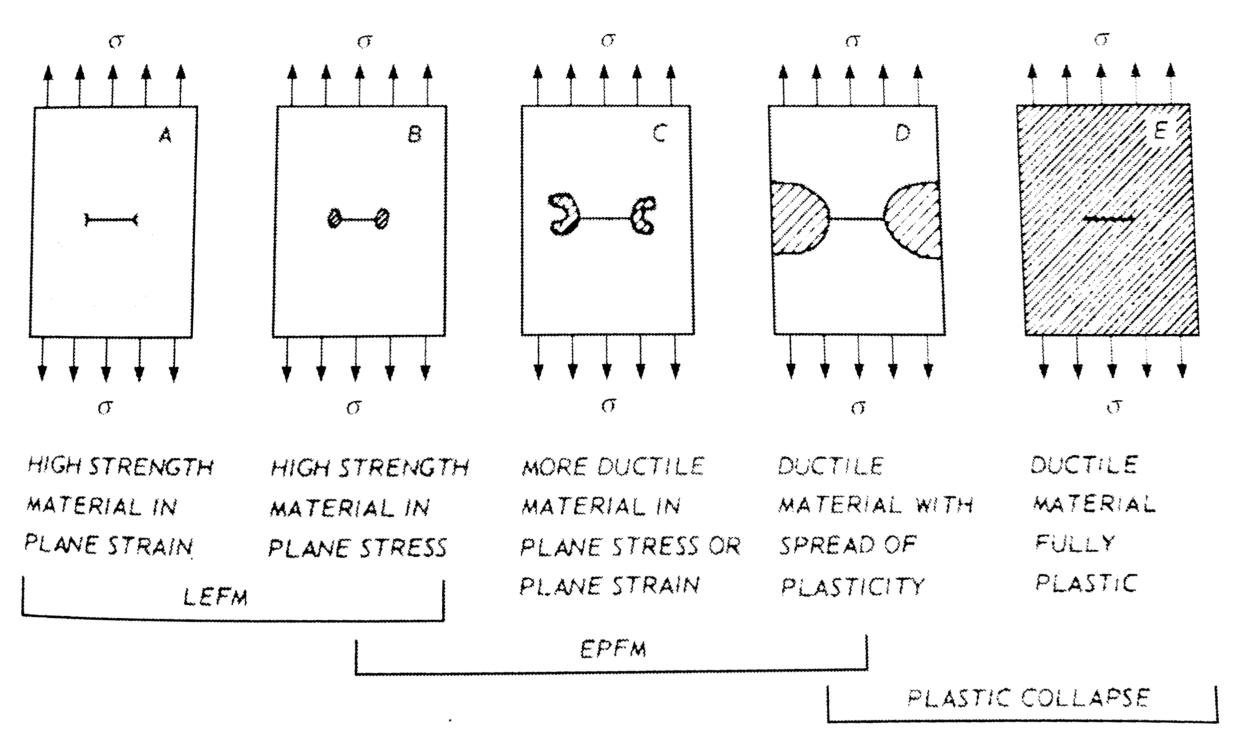
\includegraphics[width=\columnwidth]{lefm-epfm-fp-2}
\caption{Categories of Fracture Mechanics Behaviors}
\end{figure}
\end{column}
\begin{column}{0.3\textwidth}
\begin{itemize}
\item Fracture mechanics regime classified by plastic zone size
\item Linear elastic and fully-plastic are easier to model, but elastic-plastic is common in tough materials
\end{itemize}
\end{column}
\end{columns}
\note{
Fracture mechanics of a cracked body can be divided up into three main regimes:
\vfill
Linear elastic
\vfill
Elastic-plastic
\vfill
and fully-plastic, or plastic collapse.
\vfill
Each of these regimes are characterized by how much material near the crack tip has permanent plastic deformation:
\vfill
For linear elastic, there's very little material that is plastically deformed.
\vfill
For fully-plastic, a large region has plastically deformed.
\vfill
And the elastic-plastic regime is in the middle.
\vfill
Many high-performance, tough materials fall into the elastic-plastic regime. Materials in the linear elastic regime are often brittle, and materials in the fully-plastic regime severely deform once they reach their yield strength.
\vfill
}
\end{frame}

\begin{frame}
\begin{columns}
\begin{column}{0.45\textwidth}
\begin{figure}
\centering
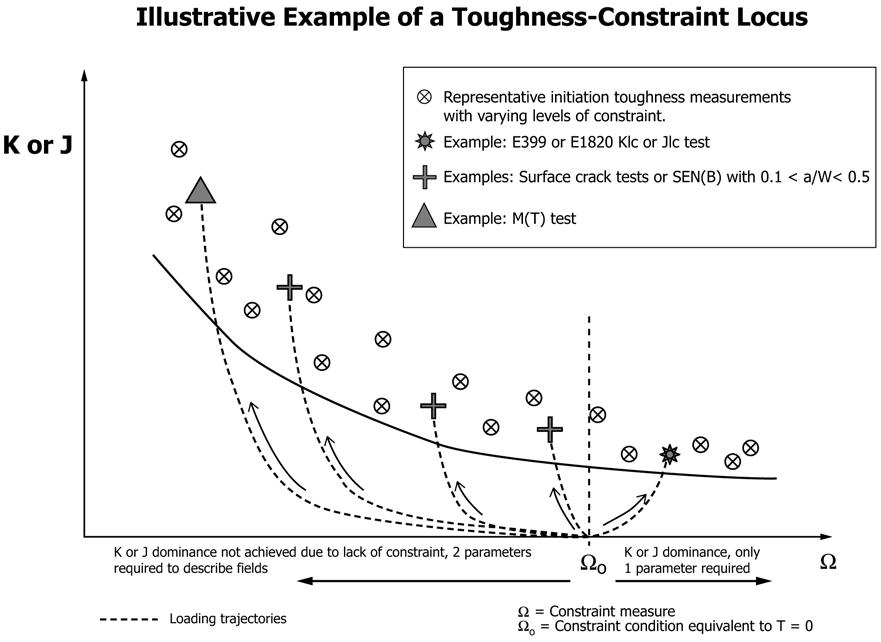
\includegraphics[width=\columnwidth]{toughness-constraint-locus}
\caption{Effect of Constraint on Fracture Toughness}
\end{figure}
\end{column}
\begin{column}{0.45\textwidth}
State of stress (constraint) near the crack tip can affect fracture toughness
\begin{itemize}
\item high constraint enables high stress without large plastic zone size, toughness is simple material property
\item low (negative) constraint increases fracture toughness, toughness is property of material and geometry (or stress state)
\end{itemize}
\end{column}
\end{columns}
\note{
Though I've just described some materials as tough, the measured toughness is not purely a material property.
\vfill
The measured fracture toughness of a sample, or of a real part, is really a property of both the material and the state of stress at the crack tip.
\vfill
Very thick bodies exhibit a high level of constraint, and can exhibit very high stress for their plastic zone size. This tends to lead to conservative estimates of fracture toughness.
\vfill
Very thin bodies with lower levels of constraint can show much higher fracture toughness values, and the measured values can vary, even for the same material. Here, fracture toughness is a property of both the material and the state of stress at the crack tip.
\vfill
}
\end{frame}

\begin{frame}
\begin{columns}
\begin{column}{0.45\textwidth}
\begin{itemize}
\item Constraint and stress states can get pretty involved.
\item Semi-elliptical surface cracks (SC01) are among the simplest part-through crack cases, and are the subject of ASTM E2899.
\item Handbook or curve-fit solutions exist for the other geometries, but only for linear elastic materials.
\item NASA's TASC program covers elastic-plastic surface cracks in tension, but {\bfseries not} in bending.
\end{itemize}
\end{column}
\begin{column}{0.45\textwidth}
\begin{figure}[tbp]
\centering
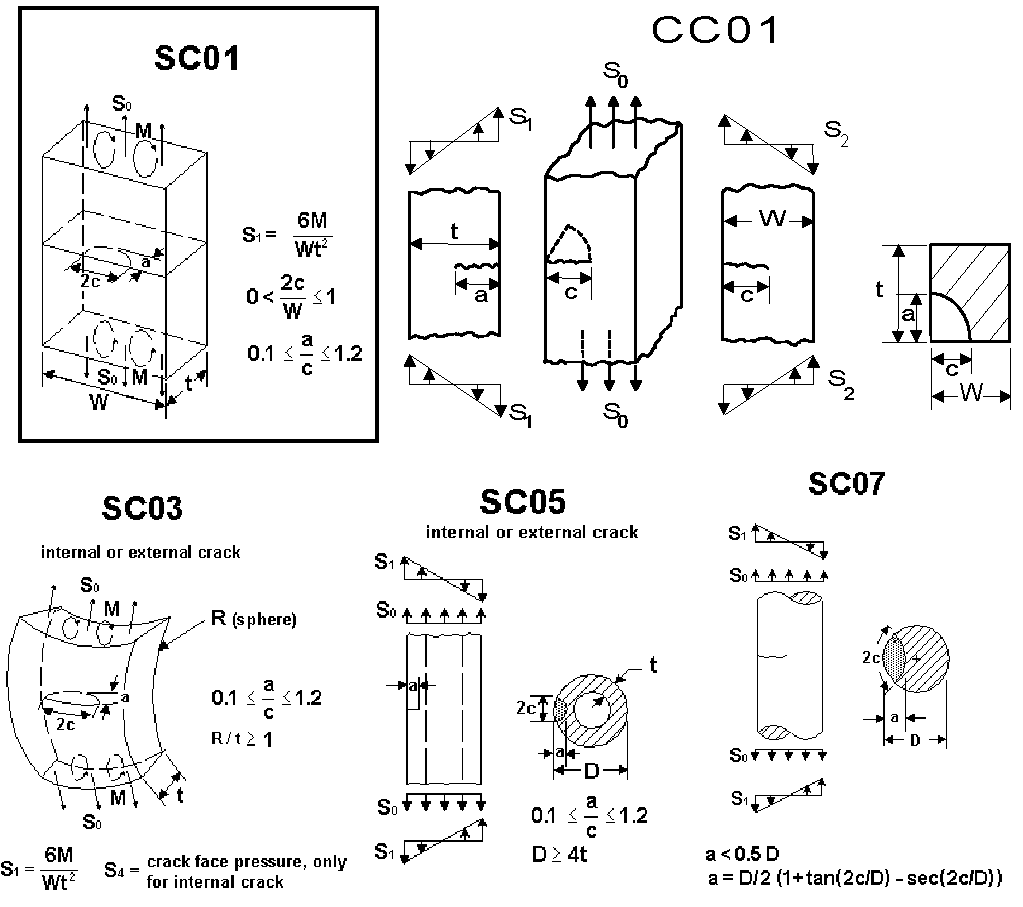
\includegraphics[width=\columnwidth]{nasgro-geometries}
\end{figure}
\end{column}
\end{columns}

\note{
The state of stress around some cracks can get pretty complicated.
\vfill
There's already been a lot of work done on geometries where the cracks go all the way through the part
\vfill
Among the part-through crack geometries shown here, the semi-elliptical surface crack is one of the simplest, and is the subject of ASTM E2899
\vfill
Handbook or curve-fit solutions exist for the other crack geometries, but only in the linear elastic regime.
\vfill
For elastic-plastic materials, the NASA TASC program covers semi-elliptical surface cracks, but only for pure tension, not for bending.
\vfill
}
\end{frame}

\begin{frame}
Research goals
\begin{itemize}
\item High quality set of elastic-plastic finite element analysis results as a basis for curve-fit or handbook calculations
\item Modified TASC program for bending or tension analysis
\item Investigation of EPRI and load separation estimation techniques
\end{itemize}
\note{
So the primary goals of this research are:
\vfill
A verified and validated set of bending models comparable to the TASC's tension models
\vfill
A modified version of TASC that works for both tension and bending
\vfill
And an investigation of two other estimation techniques for elastic-plastic fracture: EPRI and load separation
\vfill
}
\end{frame}

\part{Literature Review}

\section{Consensus Bending Stress Intensity Solution}

\begin{frame}
\begin{columns}
\begin{column}{0.65\textwidth}
For a surface crack in bending, stress intensity at a given location:
\begin{align*}
\KI &= (
        H \sigma_\text{b} F_\text{b}
        ) \left(\frac{\pi a}{Z}\right)^{0.5} \\
\sigma_\text{b} &= \frac{6 M}{W t^2} \\
Z &= 1 + 1.464\left(\frac{a}{c}\right)^{1.65} \\
F_\text{b} &= \left[ M_1 + M_2 \left( \frac{a}{t} \right)^2 + M_3 \left( \frac{a}{t} \right)^4 \right] f_\phi f_\text{wb} g \\
\end{align*}
...plus another 12 equations, and that's just for linear elastic materials.
\end{column}
\begin{column}{0.3\textwidth}
\vbox to .8\textheight{ % https://tex.stackexchange.com/questions/15244/why-does-vfill-not-work-inside-a-beamer-column
\vfill

For surface cracks in tension, we need ``only'' 10 equations.

\vfill

No such curve fit exists for elastic-plastic materials.

\vfill}
\end{column}
\end{columns}
\note{
The best consensus solution for stress intensity factors for surface cracks in bending is partially given here.
\vfill
It starts out simply enough, but the various correction factors just pile up on each other
\vfill
and it's just curve-fit after curve-fit covering 16 equations.
\vfill
Tension cases only require 10 equations, and neither of these cover elastic-plastic materials.
\vfill
}
\end{frame}

\section{Failure Assessment Diagrams and Fitness for Purpose Standards}

\begin{frame}
Failure assessment diagram: typically a graph of ratio of stress and stress intensity versus critical values
\begin{columns}
\begin{column}{0.45\textwidth}
\begin{figure}
\centering
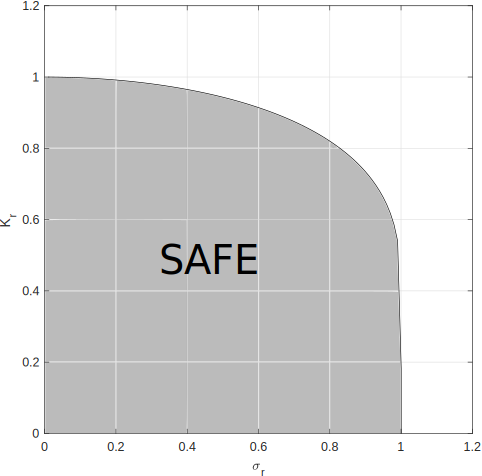
\includegraphics[width=0.6\columnwidth]{strip-yield-fad-modified}
\caption{\label{fig:strip-yield-fad} FAD using strip yield model}
\end{figure}
\end{column}
\begin{column}{0.45\textwidth}
\begin{figure}
\centering
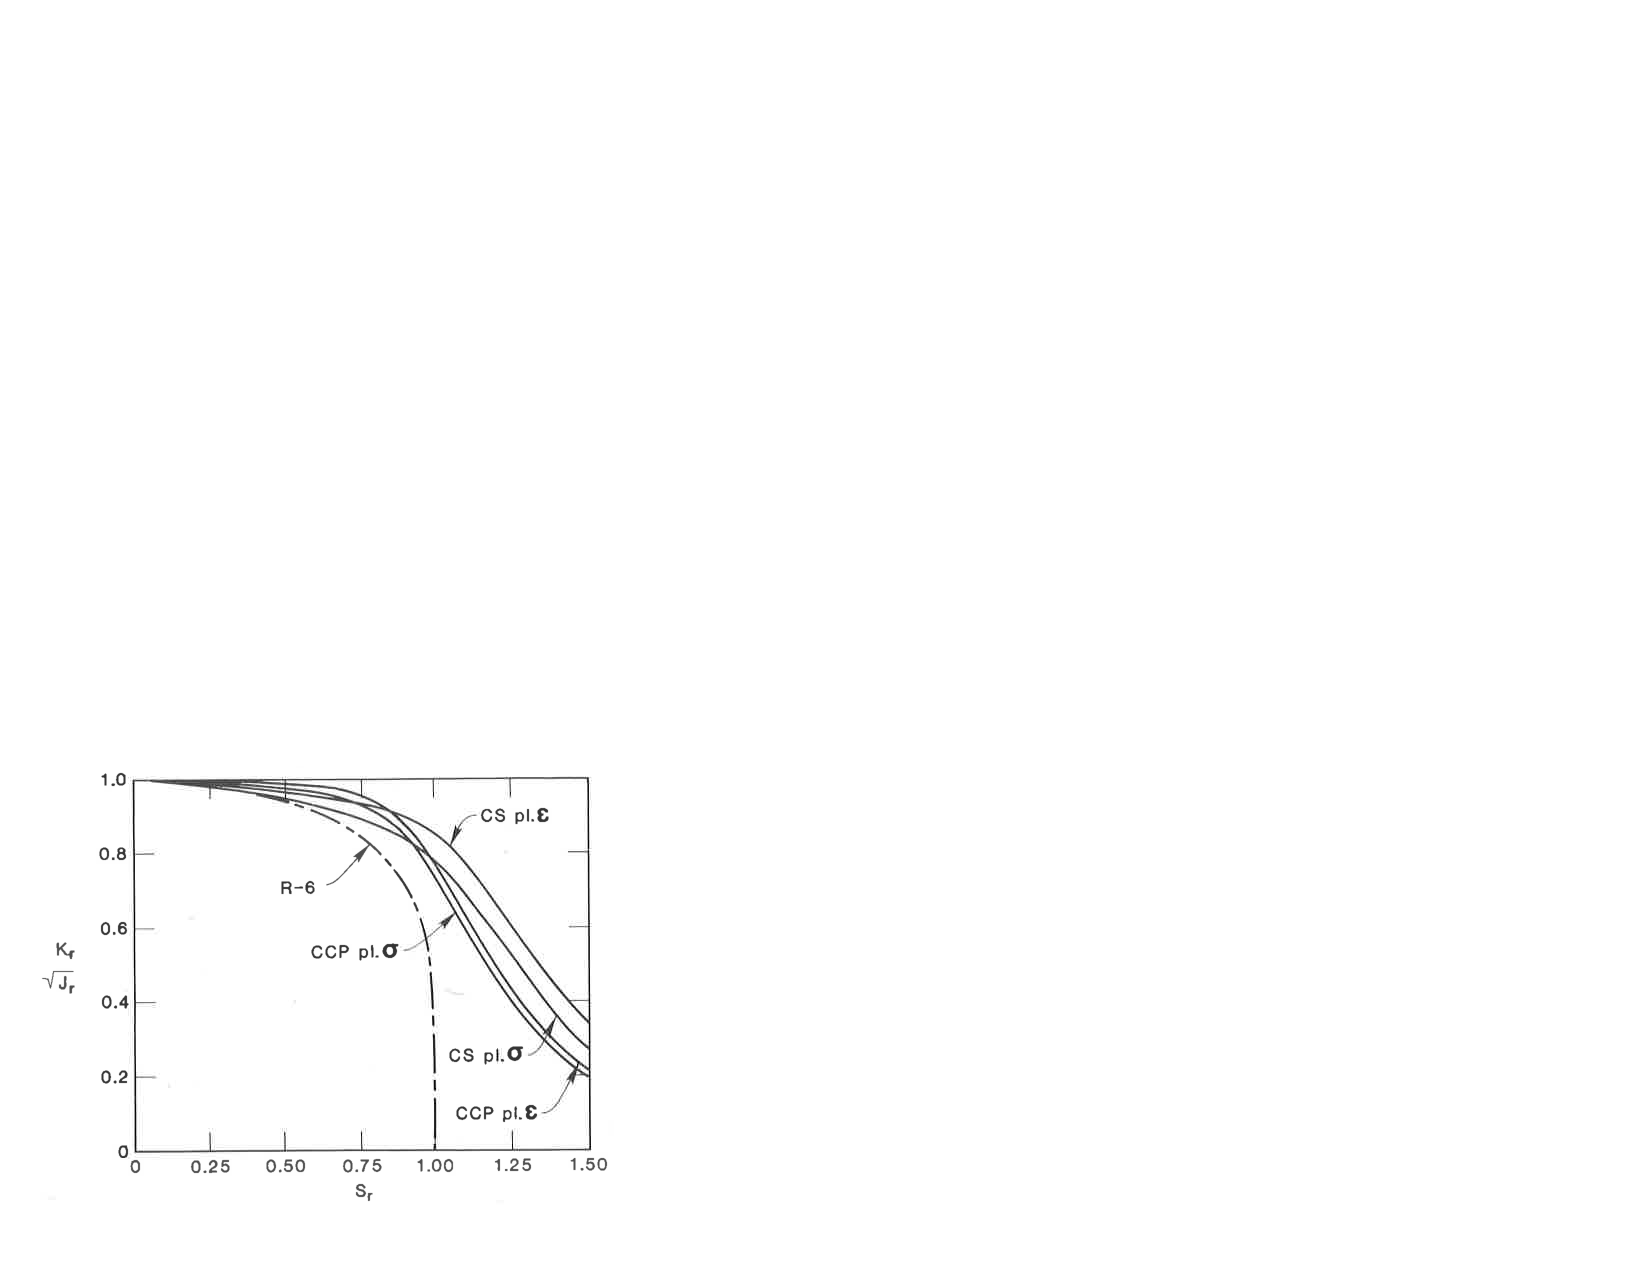
\includegraphics[width=0.7\columnwidth]{fad-for-ccp-and-ct}
\caption{\label{fig:fad-ccp-ct} FAD for two geometries and strain-hardening material}
\end{figure}
\end{column}
\end{columns}
\note{
A failure assessment diagram is one way of predicting when material failure will occur.
\vfill
A naive fracture model might assume that exceeding either a critical stress horizontally or a critical stress intensity vertically would cause failure.
\vfill
Materials with plasticity make that more complicated.
\vfill
And if a material has any strain-hardening properties, or if we have sufficiently low levels of constraint due to geometry or state of stress, the set of curves on the right is more typical.
\vfill
}
\end{frame}

\section{Constraint and Two-Parameter Fracture}

\begin{frame}
\begin{columns}
\begin{column}{0.45\textwidth}
Williams \T stress affecting normal stress in \(x\) direction (and \(z\) direction for plane strain):
\begin{align*}
\sigma_{ij} &= \frac{\KI}{\sqrt{2\pi r}} f_{ij}(\theta) +
\begin{bmatrix}
T & 0 & 0 \\
0 & 0 & 0 \\
0 & 0 & \nu \T
\end{bmatrix}
\label{eq:t-stress}
\end{align*}
affects plastic zone size and fracture toughness, varies with geometry and loading condition, applies to linear elastic materials (and is relatively accurate for elastic-plastic materials).
\end{column}
\begin{column}{0.45\textwidth}
\begin{figure}
\centering
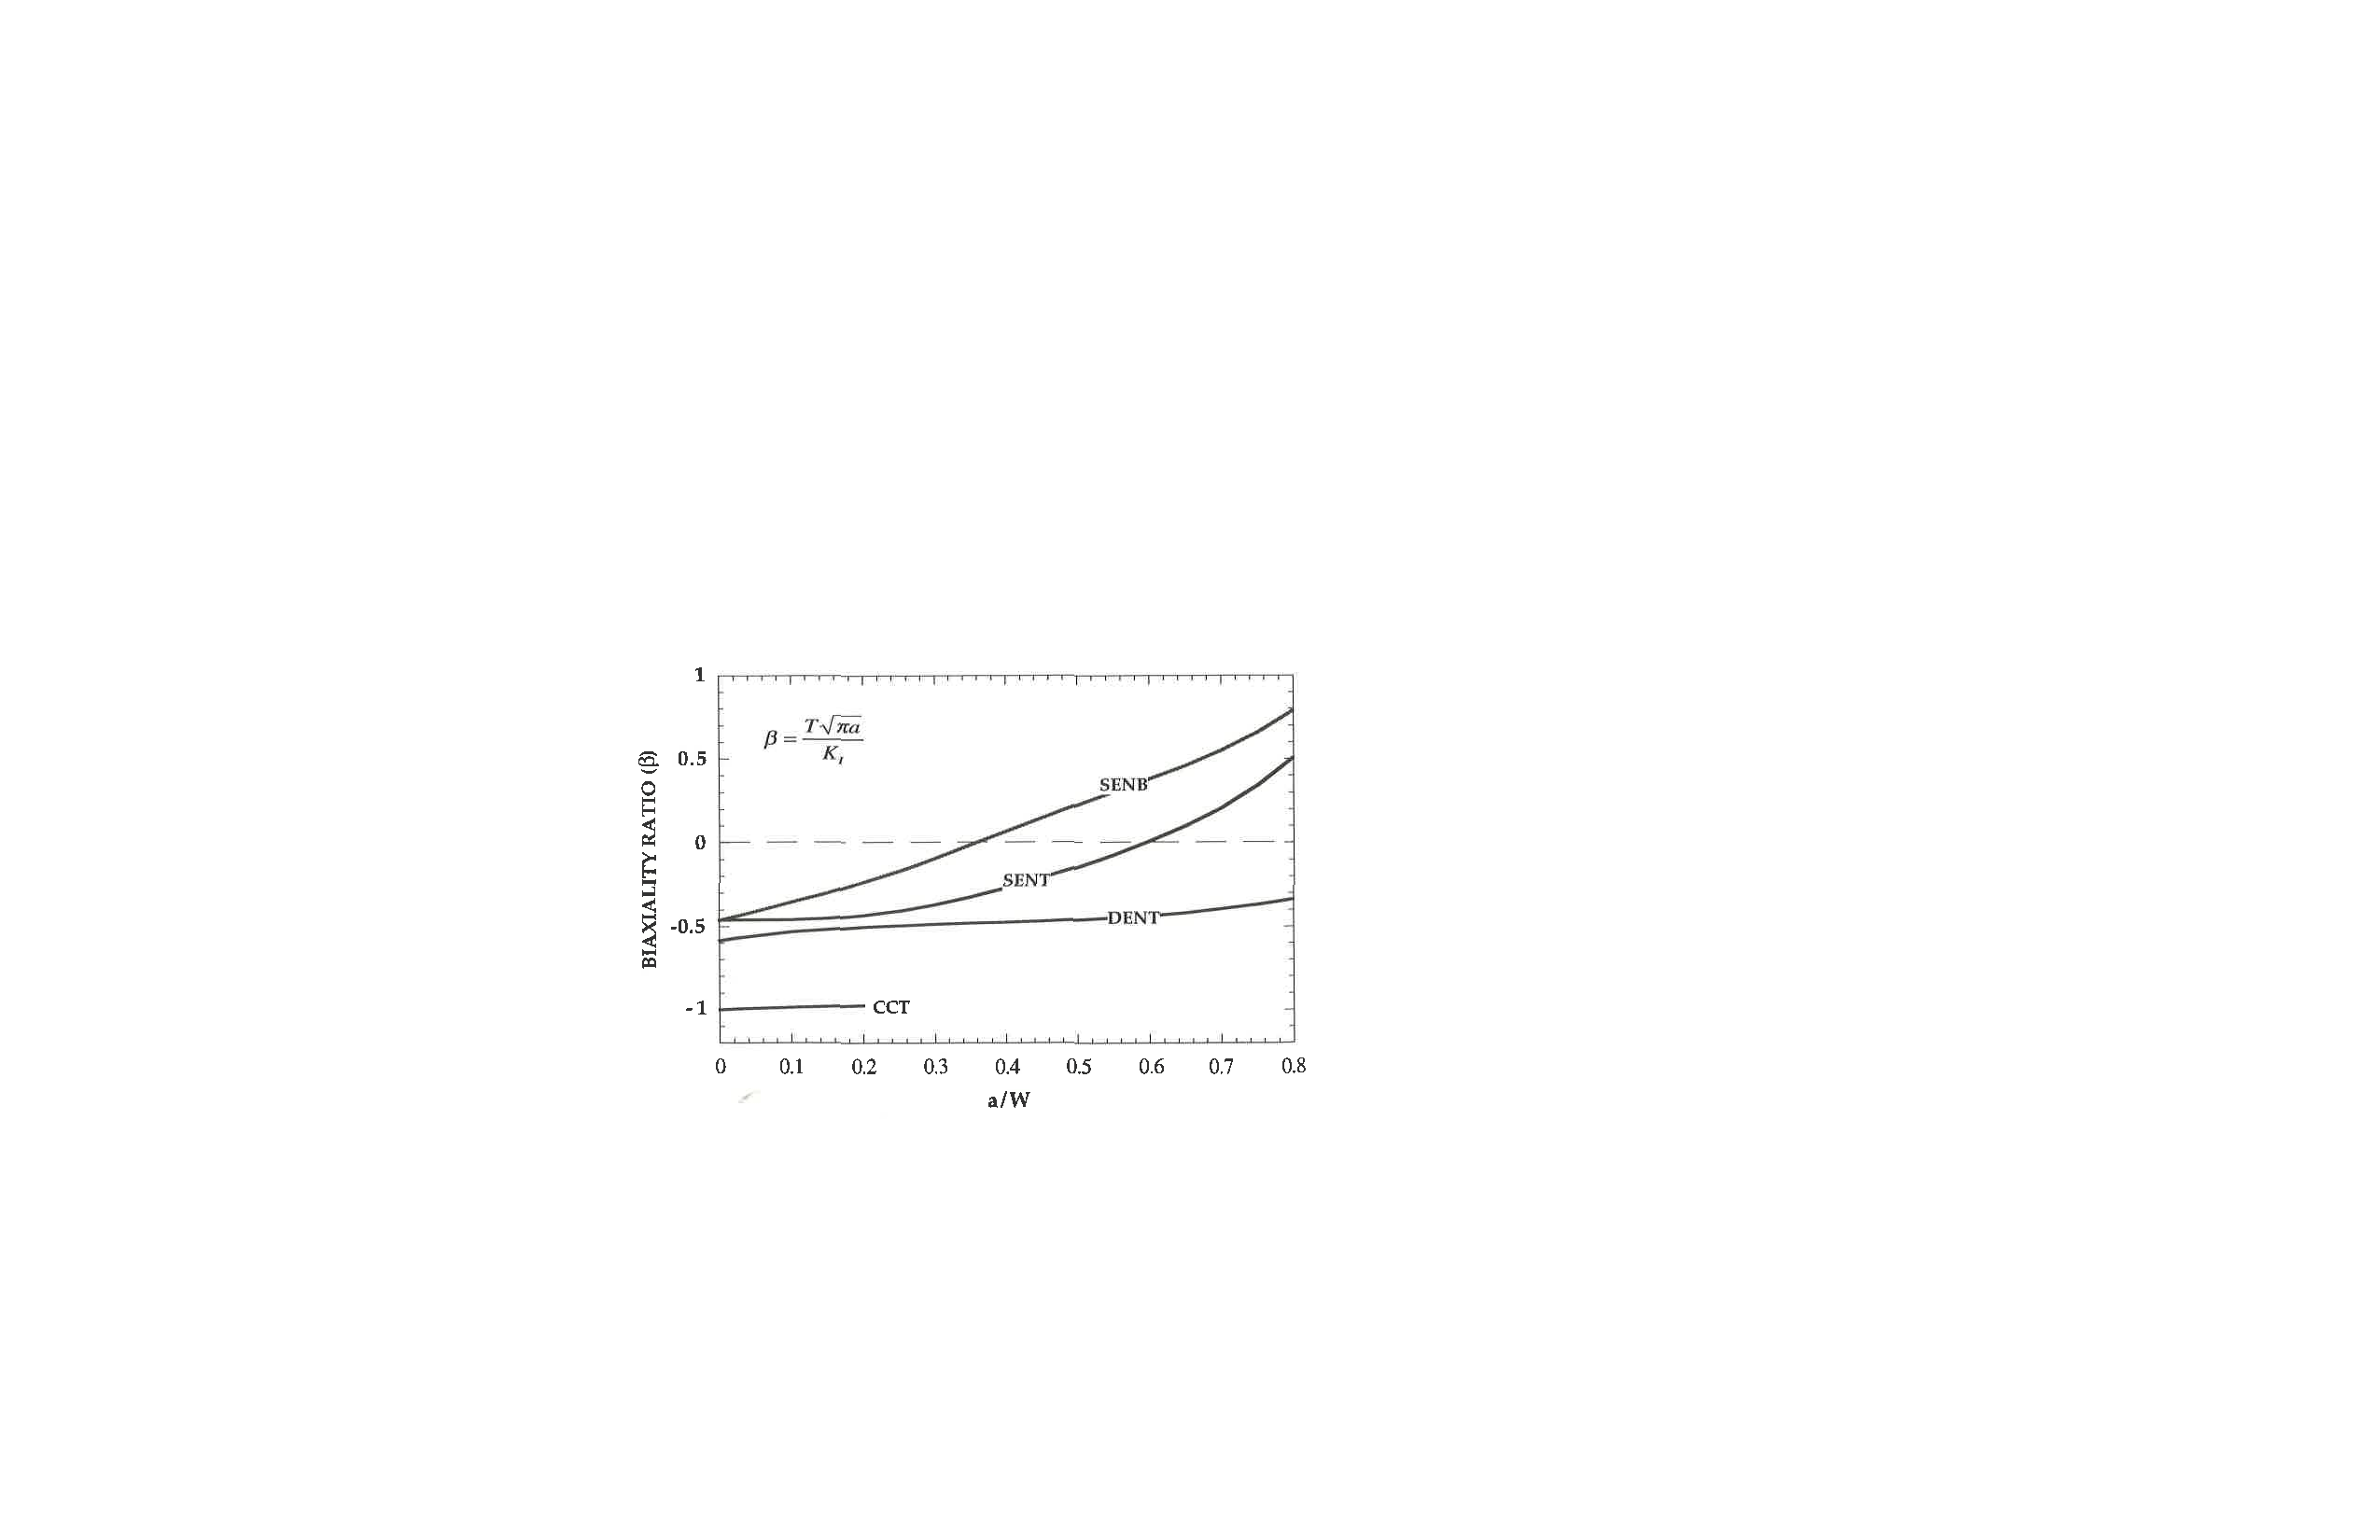
\includegraphics[width=\columnwidth]{biaxiality}
\caption{\label{fig:biaxiality} Biaxiality ratio for various specimens}
\end{figure}
\end{column}
\end{columns}
\note{
One way to characterize constraint is a \T stress acting in the \(x\) direction (that is, the direction of crack growth).
\vfill
That stress will affect the size of the plastic zone, and varies with geometry and loading condition as seen in the figure on the right.
\vfill
Specimens cracked on a single edge loaded in tension or bending have the most variation in \T stress as cracks grow larger.
\vfill
}
\end{frame}

\section[Methods for EP and FP Bending Analysis]{Methods for Elastic-Plastic and Fully-Plastic Bending Analysis}

\subsection{Numerical Methods}

\begin{frame}
\begin{columns}
\begin{column}{0.45\textwidth}
\begin{figure}[tbp]
\centering
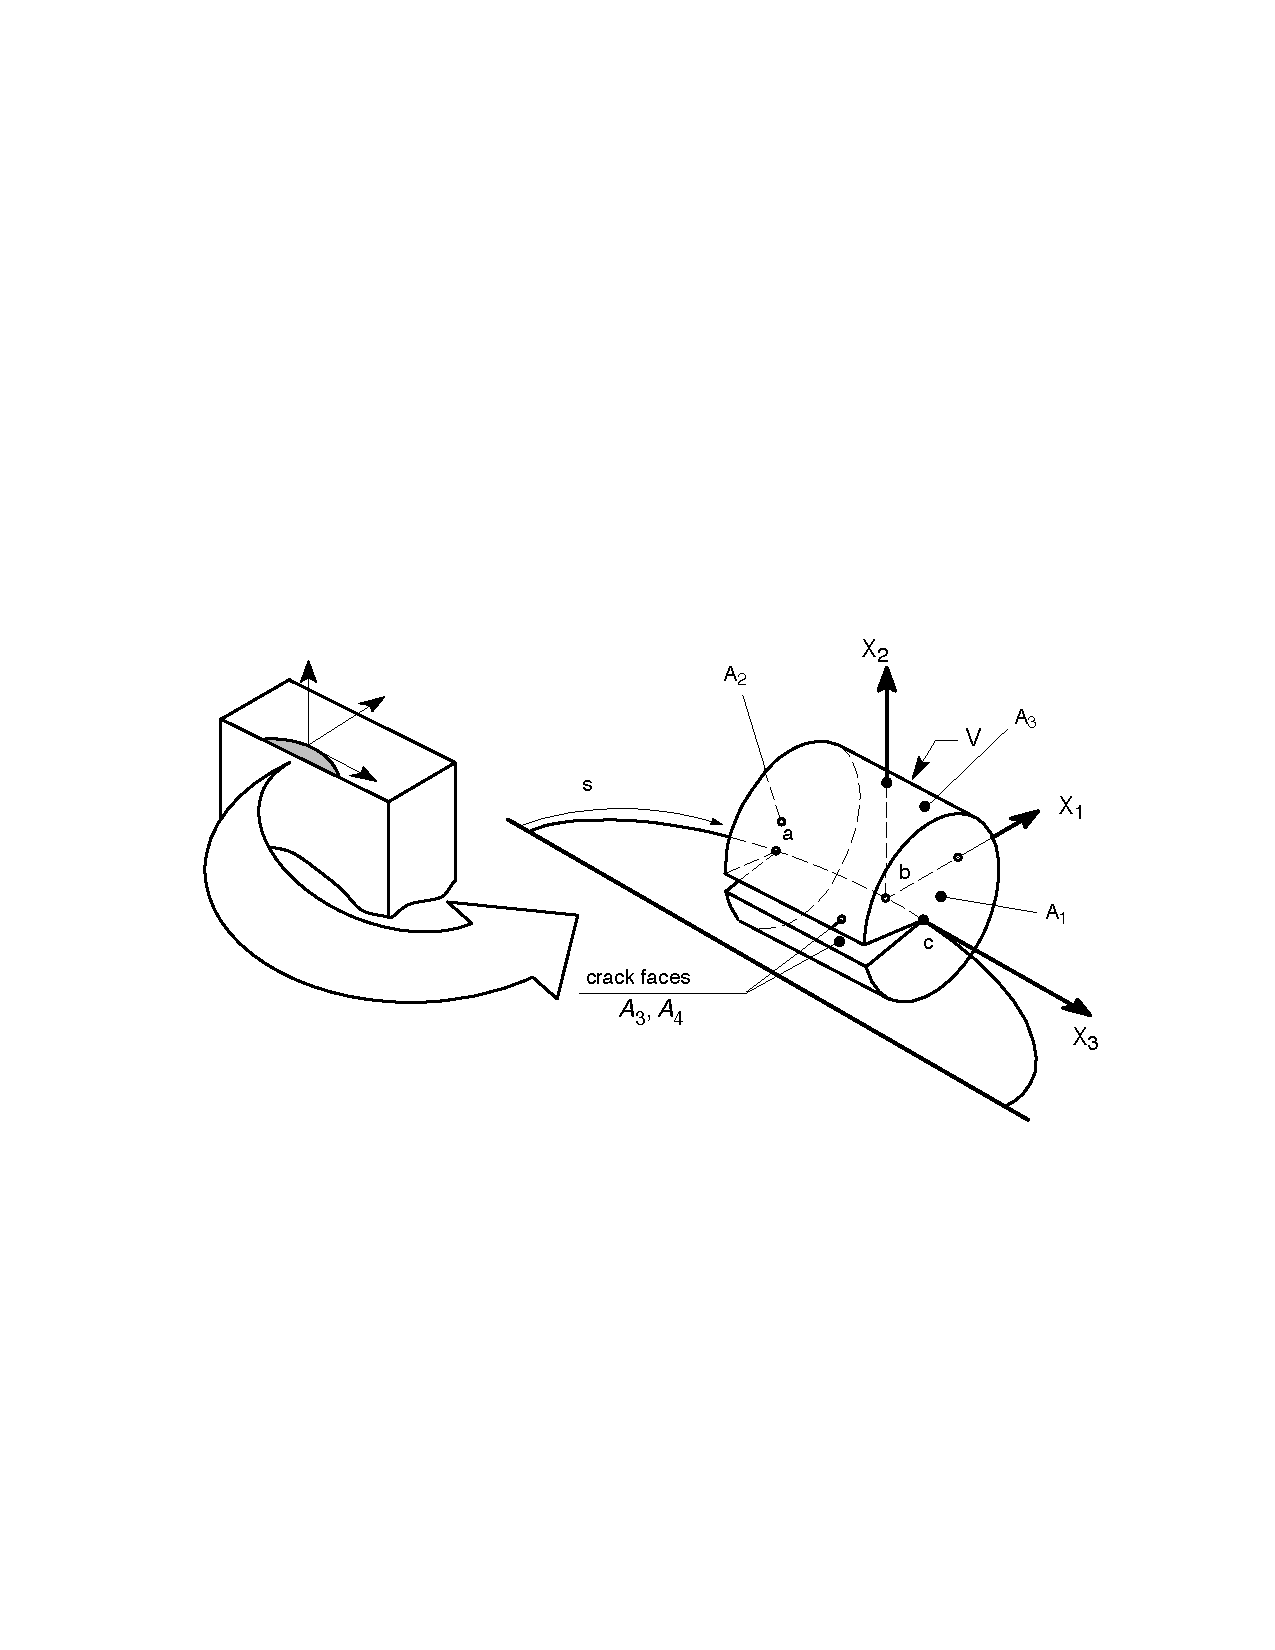
\includegraphics[width=\columnwidth]{domain-integral-volume}
\caption{Example of a domain integral volume for numerically calculating \J}
\end{figure}
\end{column}
\begin{column}{0.45\textwidth}
The contour integral form of \J
\begin{align*}
\J &= \int_{\Gamma} \left( w \, {dy} - T_i \pderiv{u_i}{x} \, {ds}\right)
\end{align*}
can be converted to a discretized version using a group of elements surrounding a point on the crack front
\begin{align*}
J &= \sum_{\substack{\text{all elements}\\\text{in domain}}} \, \sum_{p=1}^{m}
      f \left( 
        \sigma, \epsilon, u
      \right)
\end{align*}
using \(m\) Gauss points in each element.
\end{column}
\end{columns}
\note{
The elastic-plastic fracture parameter \J was originally defined in terms of a contour integral in 2D, or a surface integral in 3D.
\vfill
In a finite element analysis code, this can be converted to a version including stress, strain, and deformation values from all the elements surrounding a location along the crack front.
\vfill
There's a lot more detail in that f function, but that's the high-level version of it.
\vfill
}
\end{frame}

\subsection{Estimation Schemes}

\begin{frame}
EPRI estimation:
\begin{columns}
\begin{column}{0.45\textwidth}
Elastic-plastic \J as sum of elastic and fully-plastic \J components:
\begin{align*}
\J &= \Jel + \Jpl
\end{align*}
\begin{itemize}
\item \( \Jel = \frac{K^2}{E'} \) with apparent crack size
\item \( \Jpl = h_1 \left( \frac{a}{W}, n \right) \left( \frac{P}{P_0} \right)^{n+1} \alpha \epsilon_0 \sigma_0 b \) with Ramberg-Osgood material model and limit load
\end{itemize}
\end{column}
\begin{column}{0.45\textwidth}
\begin{figure}
\centering
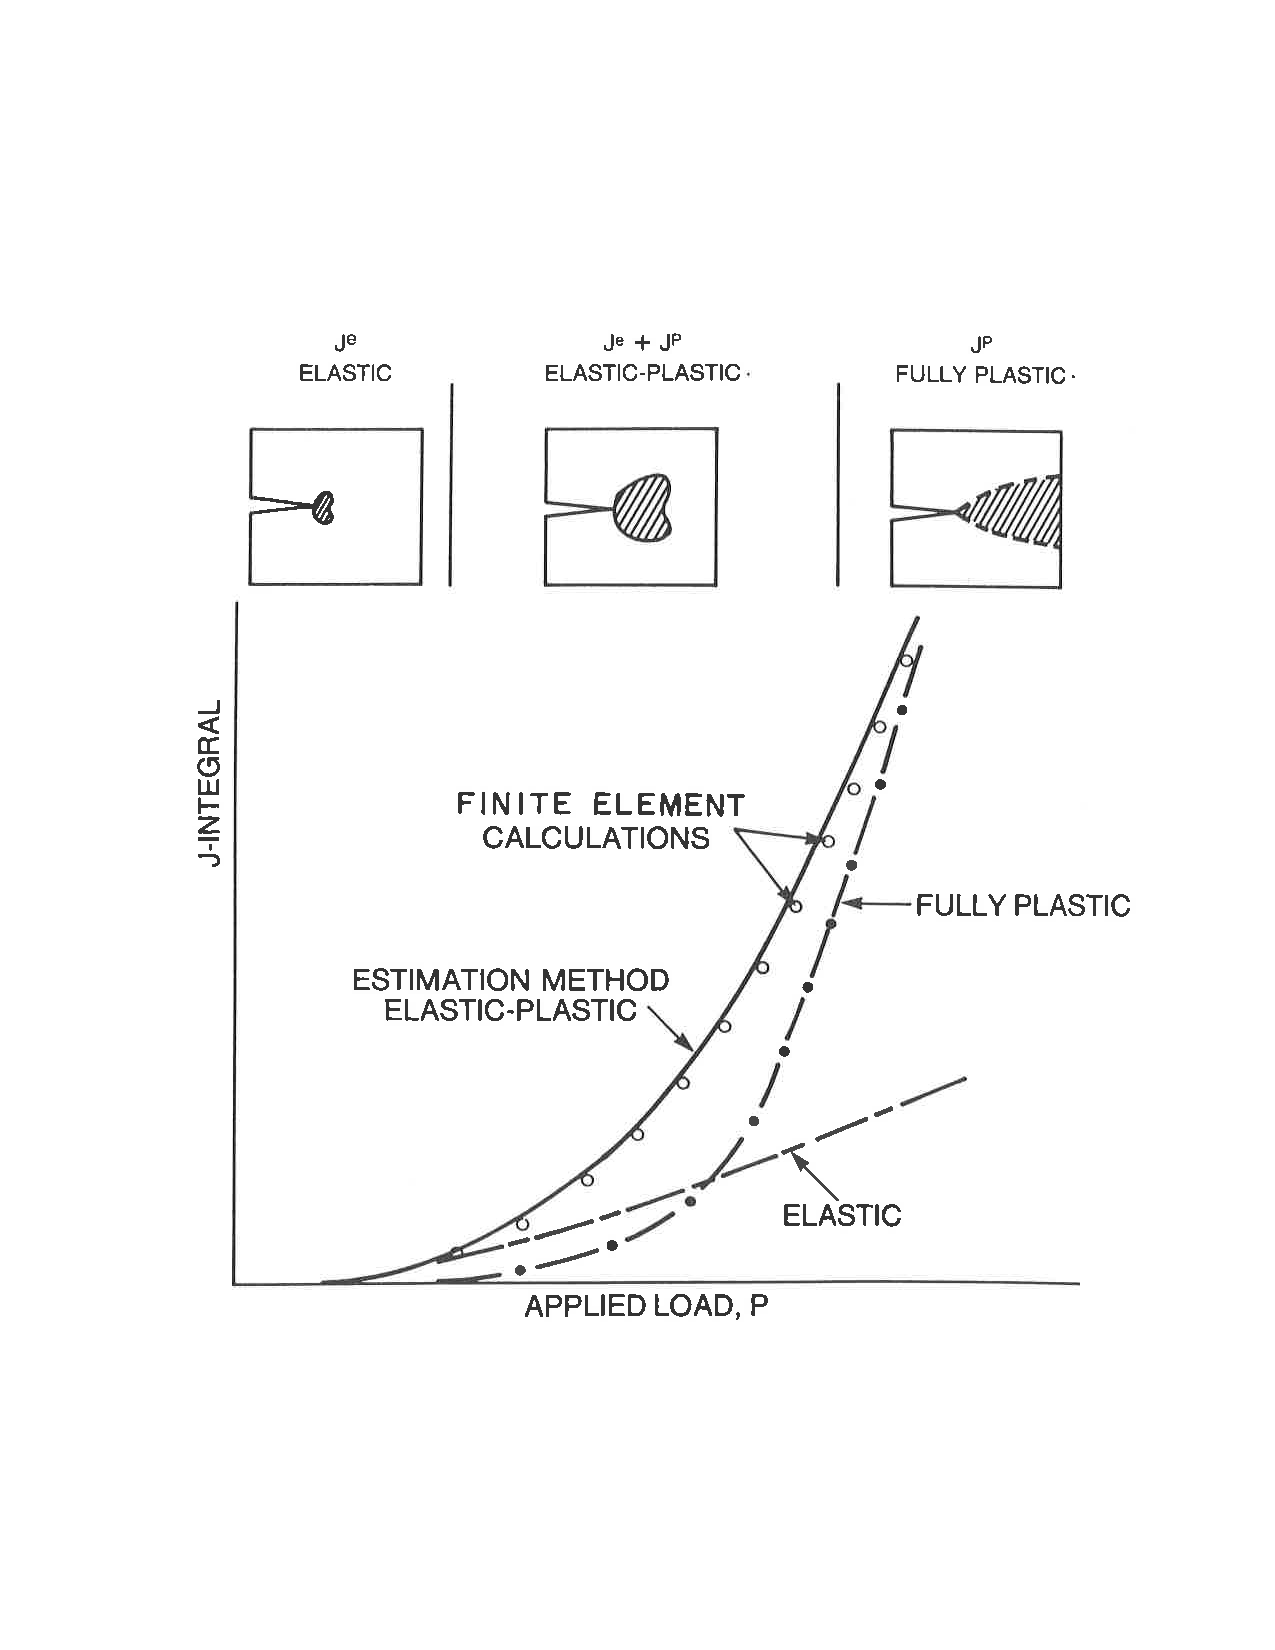
\includegraphics[width=0.8\columnwidth]{epri-scheme}
\end{figure}
\end{column}
\end{columns}
\note{
One way of estimating elastic-plastic behavior is the EPRI method,
\vfill
where linear-elastic and fully-plastic \J components are summed to a total \J value.
\vfill
Under small loads, the linear elastic component dominates.
\vfill
But as load increases, the fully-plastic component grows more rapidly and eventually contributes the vast majority of the final \J value.
\vfill
The elastic component of \J can be related back to the stress intensity factor \K, and the plastic component uses a limit load analysis and a power-law material model.
\vfill
This was originally done for 2D crack geometries, but has been applied for 3D geometries since.
\vfill
}
\end{frame}

\subsection{Load Separation}

\begin{frame}
\begin{columns}
\begin{column}{0.6\textwidth}
\begin{figure}
\centering
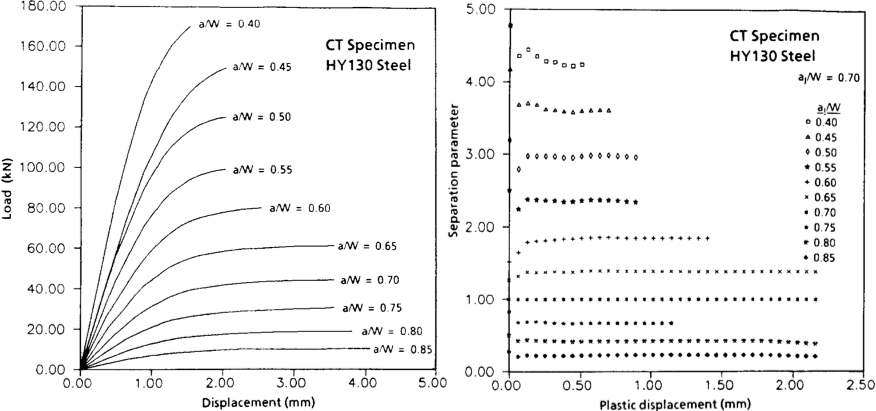
\includegraphics[width=\columnwidth]{load-separation-side}
\caption{Load separation parameter versus plastic displacement for a compact tension specimen}
\end{figure}
\end{column}
\begin{column}{0.3\textwidth}
\begin{figure}
\centering
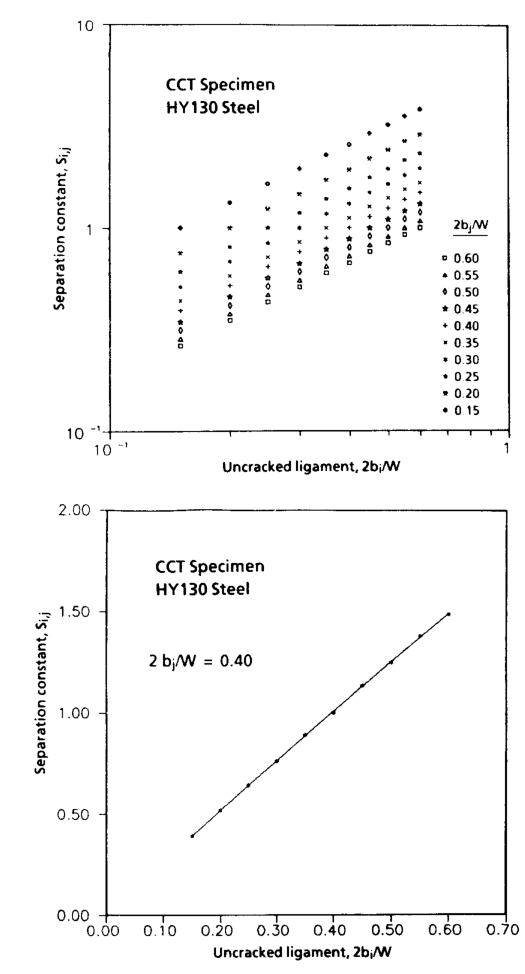
\includegraphics[width=0.7\columnwidth]{load-separation-uncracked-ligament}
\end{figure}
\end{column}
\end{columns}
\note{
Load separation attempts to separate \J into material and geometry components, similar to a separation of variables in differential equations.
\vfill
It results in a single-specimen technique where \J for any crack length can be predicted from a single test record using the same material.
\vfill
It relies on load-displacement curves converging to fixed ratios versus a given reference curve shown in the left figure,
\vfill
and being able to fit those ratios to a single curve shown in the right figure.
\vfill
This was also originally applied to 2D geometries, but has later been used for 3D cracks.
\vfill
}
\end{frame}

\section[Engineering Approaches for EP and FP Analysis of Surface Cracks]{Engineering Approaches for Elastic-Plastic and Fully-Plastic Analysis of Surface-Cracked Plates in Bending}

\subsection{ASTM E2899}

\begin{frame}
ASTM E2899: Standard Test Method for Measurement of Initiation Toughness in Surface Cracks Under Tension and Bending
\begin{columns}[b]
\begin{column}{0.45\textwidth}
\begin{figure}
\centering
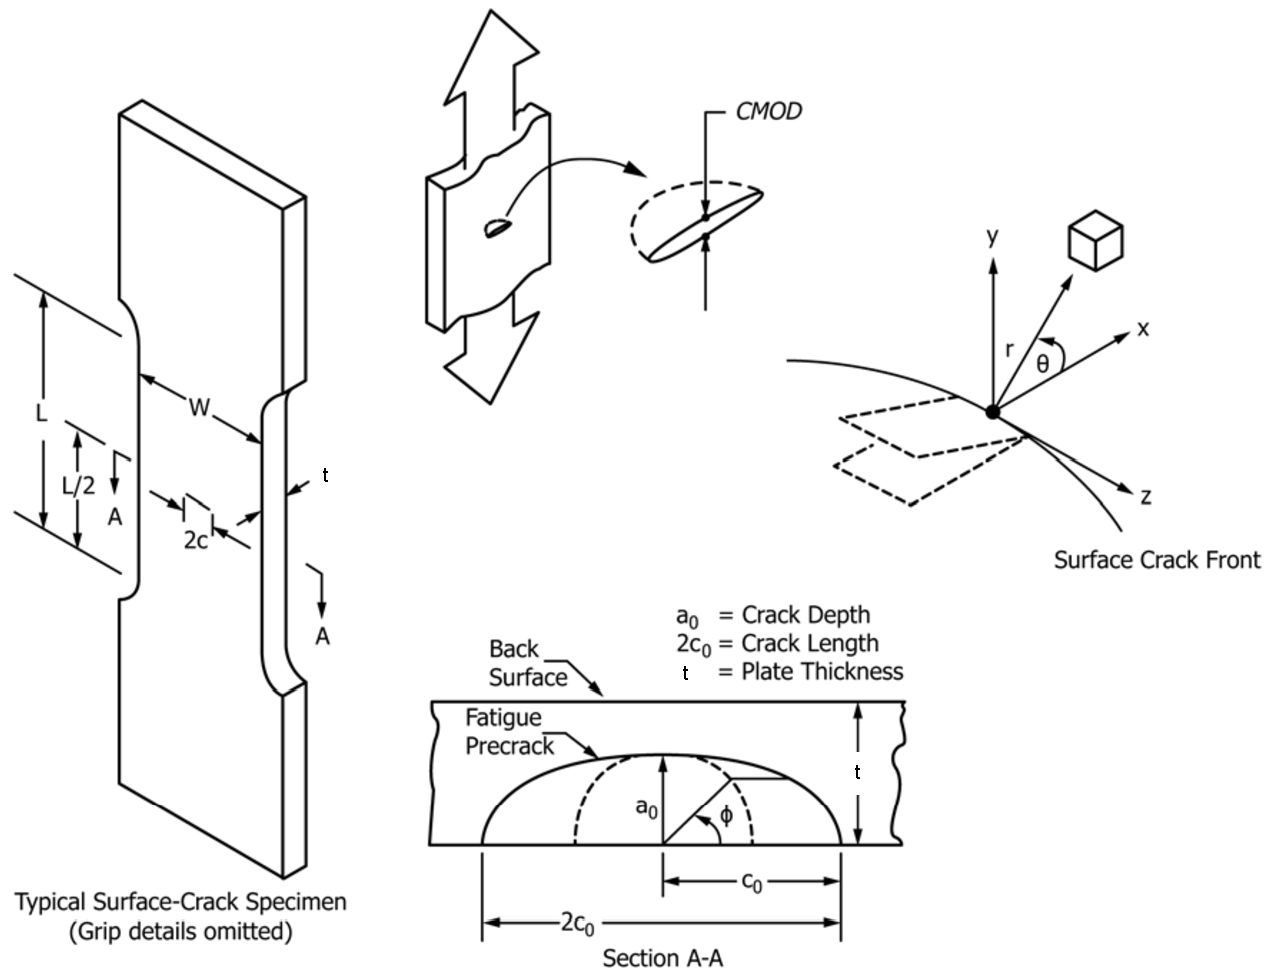
\includegraphics[width=0.9\columnwidth]{sc-terminology-e2899-modified}
\caption{Test specimen and crack configurations}
\end{figure}
\end{column}
\begin{column}{0.45\textwidth}
\begin{figure}
\centering
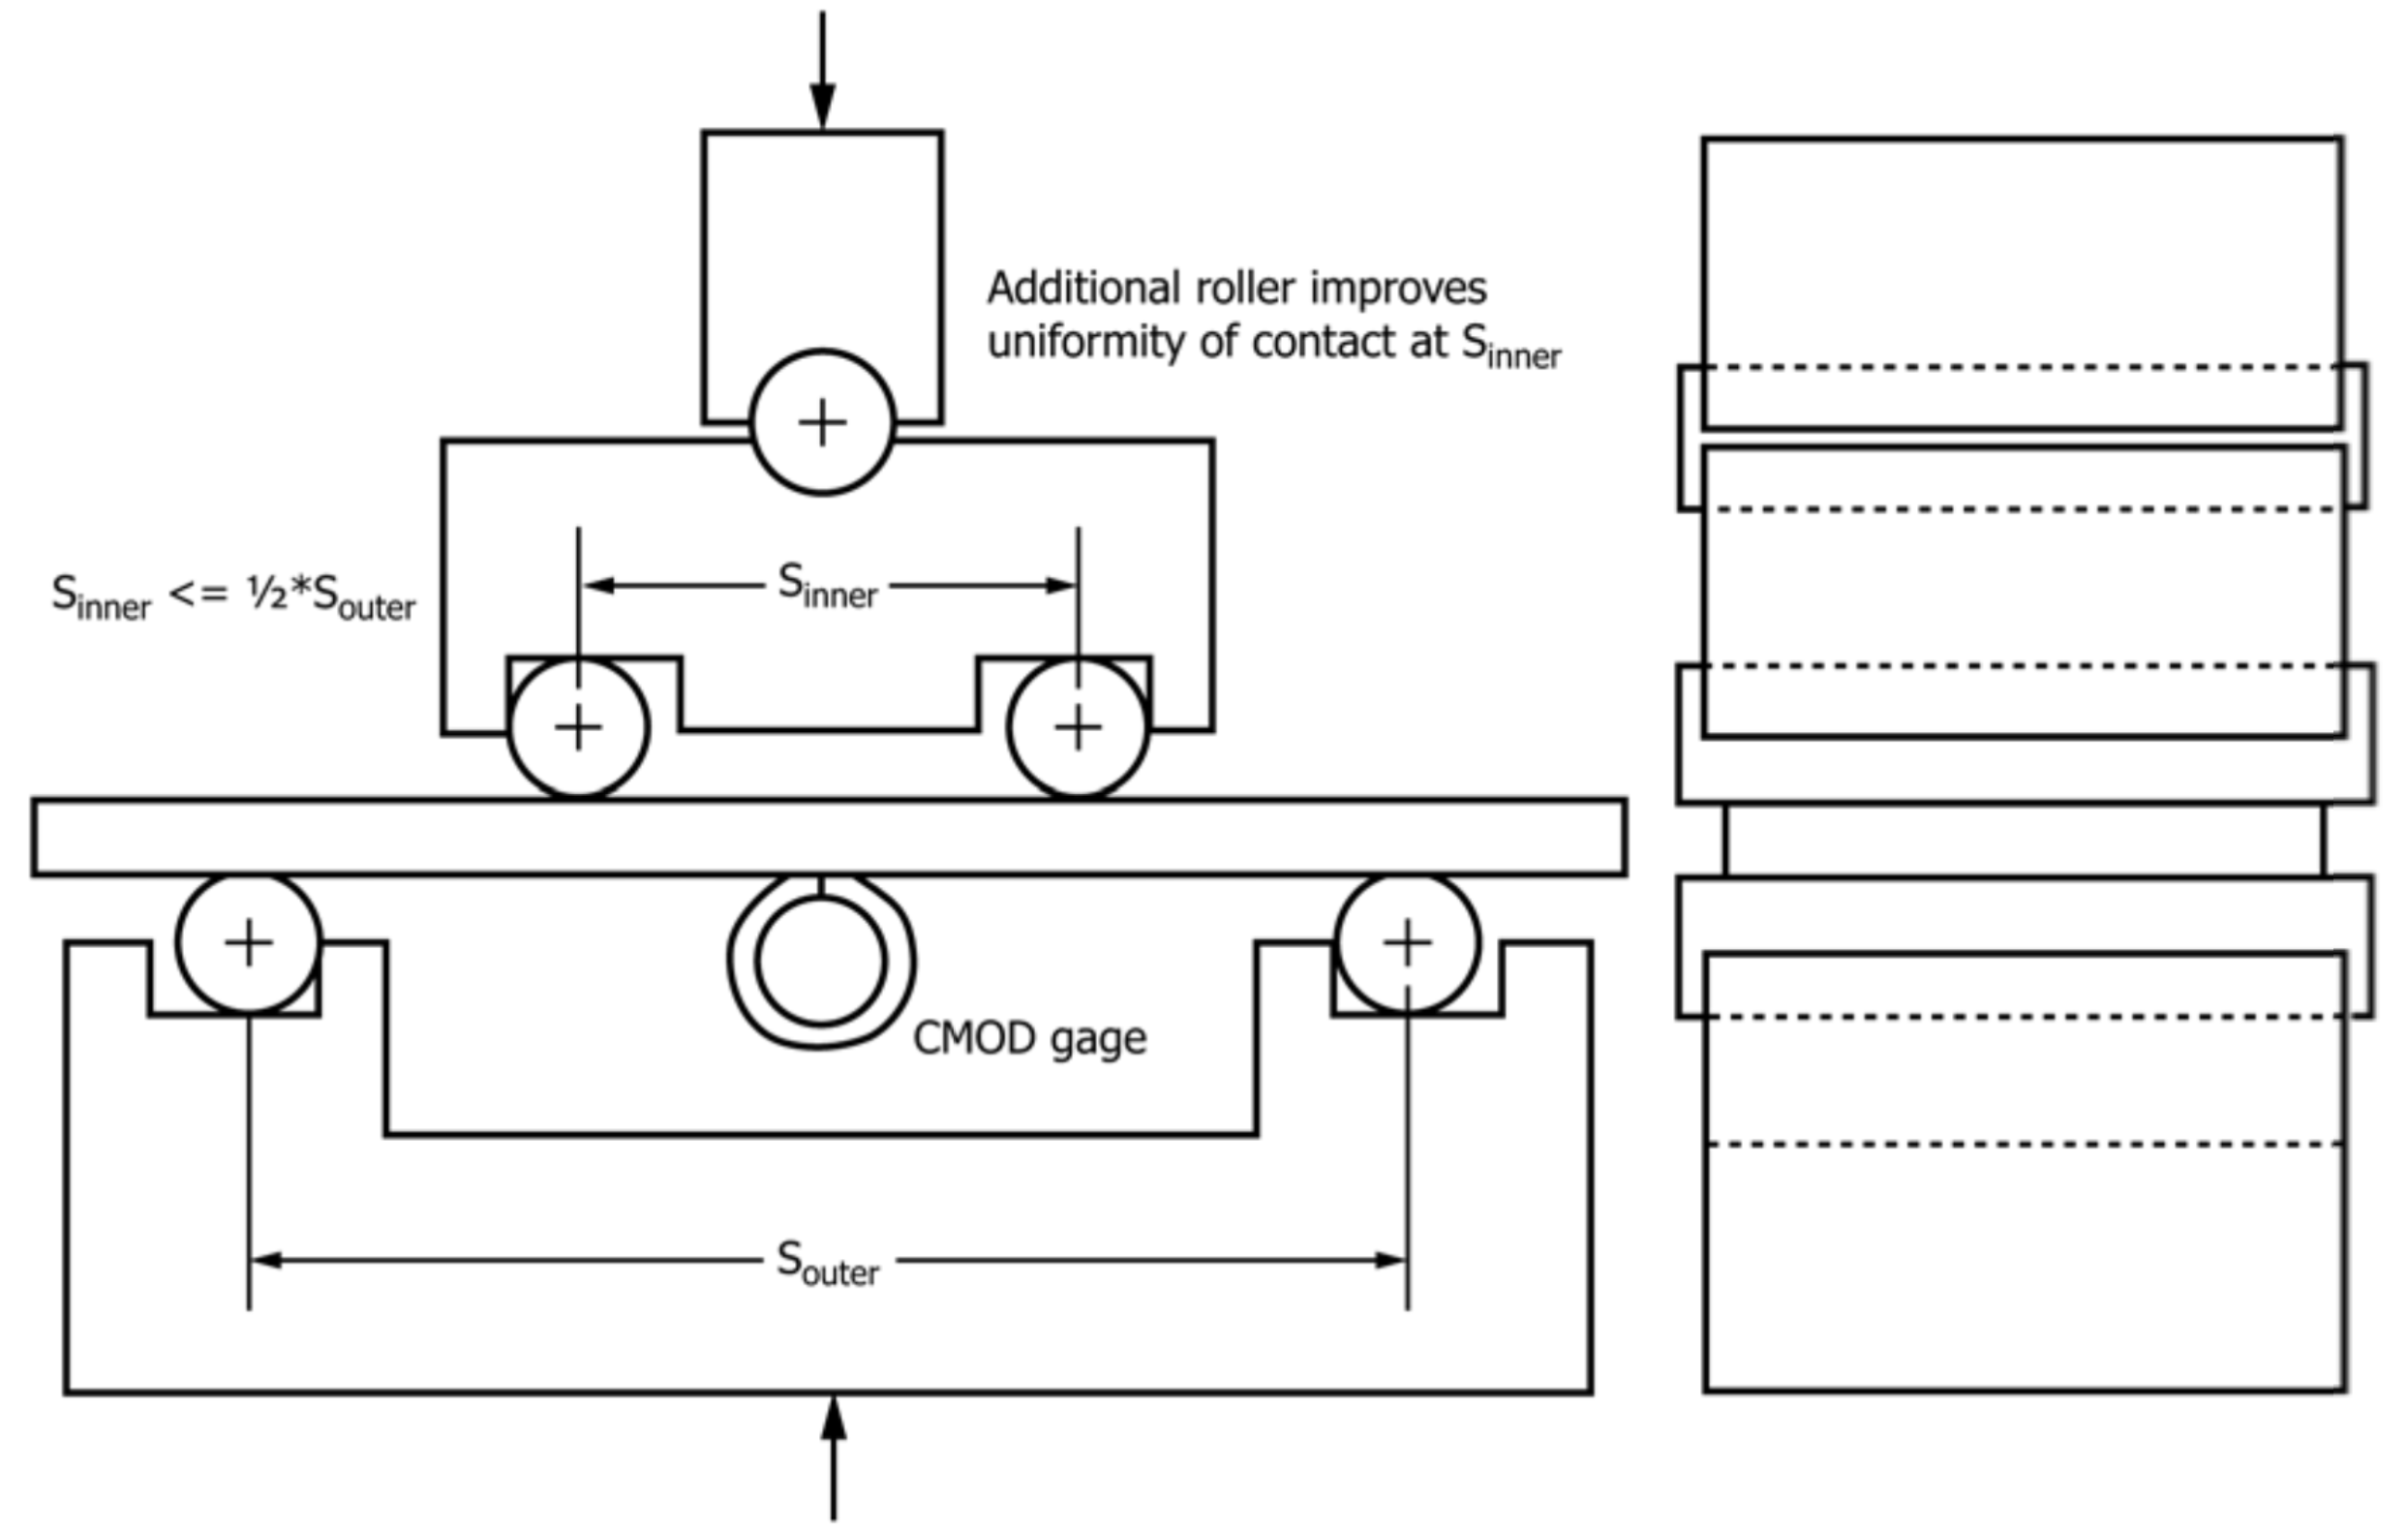
\includegraphics[width=0.9\columnwidth]{astm-e2899-4point-bend}
\caption{Four-point bend test configuration}
\end{figure}
\end{column}
\end{columns}
\note{
So now we get to the current ASTM standard for measuring fracture toughness for flat plates with surface cracks, E2899.
\vfill
On the left is an example specimen including a cross section of its semi-elliptical surface crack, and on the right is a specimen loaded into a four-point bending configuration.
\vfill
}
\end{frame}


\begin{frame}
\begin{itemize}
\item Starter crack machined into flat plate, fatigued to sharpen crack front
\item CMOD monitored as tension or bending load increased monotonically
\item Either specimen fails or start of stable crack tearing is detected
\item Location where crack growth occurs is recorded
\item Conditions classified as linear elastic, elastic-plastic, or fully-plastic
\item If LEFM or EPFM, calculate constraint from tables
\item If LEFM, calculate \K from series of provided equations
\item If EPFM, {\bfseries use nonlinear FEA} to calculate \J
\end{itemize}
\note{
In ASTM E2899, the first few steps to calculating stress conditions at the crack tip are purely related to experimental measurement.
\vfill
For linear elastic conditions, a series of equations derived from experimental curve fits can be used to calculate \K.
\vfill
But for elastic-plastic conditions, no such series of equations exists to calculate \J, and finite element analysis is required in the standard.
\vfill
This last step is a major departure compared to other standards, and would normally require construction of models for every tested geometry and material.
\vfill
}
\end{frame}

\begin{frame}
\begin{center}
Calculation or analysis requirements for other ASTM standards:

\begin{tabular}{c p{0.5\textwidth} p{0.3\textwidth}} \toprule
 & Requirements & Tools \\ \midrule
E8 & Fit linear region of stress-strain curve, offset to find yield strength & Strip chart and calculator \\
E399 & Fit linear region of force-CMOD curve, draw secant line with 5\% less slope, calculate \K with algebraic equations & Strip chart and calculator or spreadsheet \\ 
E1820 & Calculate \K with algebraic equations. EPRI method for \Jel calculated from \K, \Jpl from area under load-displacement curve and algebraic equations & Spreadsheet \\ \bottomrule
\end{tabular}
\end{center}
\note{
By comparison, other ASTM standards like E8, E399, and E1820 require much less analysis, and are fundamentally experimental with some handbook, tabular, or curve-fitted equations to calculate.
\vfill
Elastic-plastic finite element analysis is a huge departure from what people had expected from earlier standards.
\vfill}
\end{frame}

\subsection{Tool for Analysis of Surface Cracks (TASC)}

\begin{frame}
\begin{columns}
\begin{column}{0.45\textwidth}
ASTM E2899 is unusual in its analysis requirements
\begin{itemize}
\item requires results of elastic-plastic finite element analysis
\item other standards require much simpler calculations or graphical constructions
\item NASA TASC program satisfies requirements, but only for tension
\end{itemize}
Mechanics of bending is more complex than for tension (constraint, crack closure)
\end{column}
\begin{column}{0.45\textwidth}
\begin{figure}
\centering
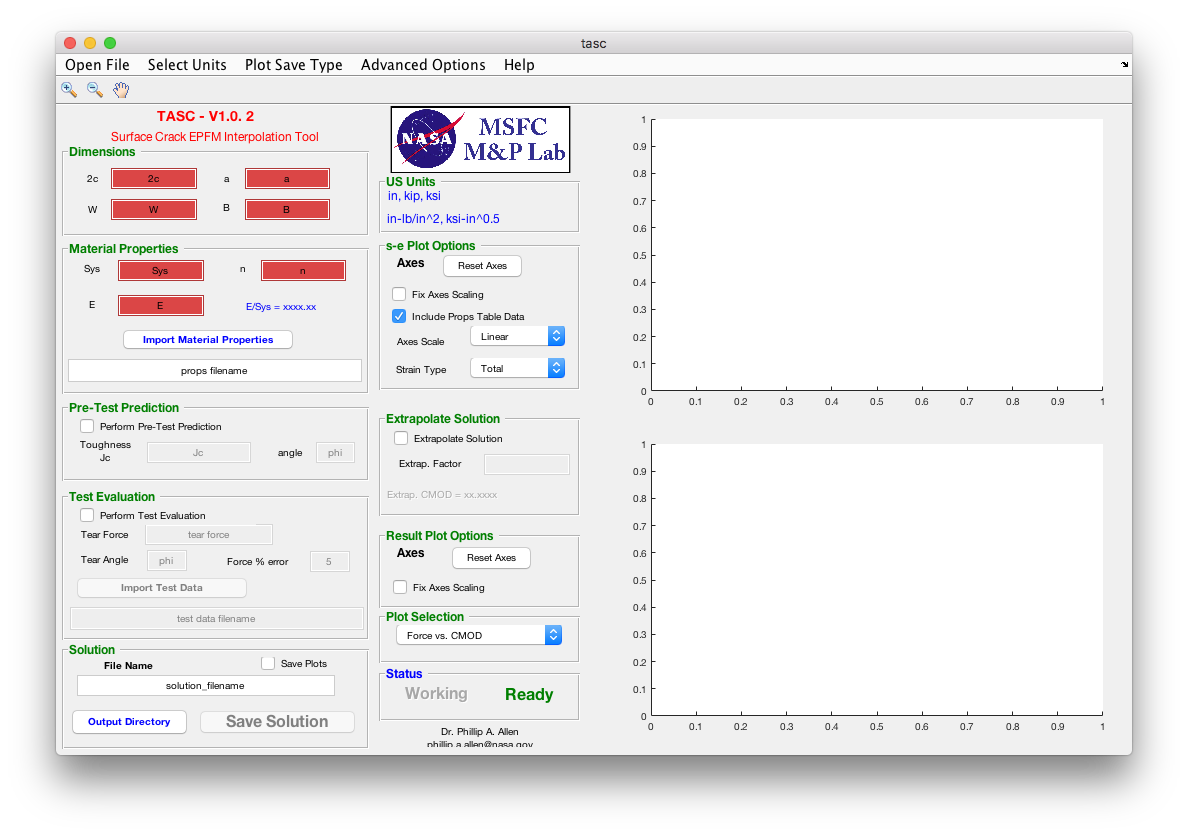
\includegraphics[width=\columnwidth]{tasc-original}
\caption{NASA TASC program}
\end{figure}
\end{column}
\end{columns}
\note{
The vast majority of ASTM standards focus on experimental techniques, with some basic graphical constructions or simple equations to verify the test was done properly
\vfill
But ASTM E2899 requires finite element analysis for elastic-plastic materials, and this can be a burden on those performing these kinds of tests.
\vfill
The NASA TASC program satisfies those analysis requirements, but only works for tension, not in bending.
\vfill
Bending analysis is more complex than tension analysis: cracks can close, and the state of stress around the crack front makes for variable constraint conditions.
\vfill
}
\end{frame}

\begin{frame}
TASC: interpolation code using database of 600 EPFM results for flat plates in tension
\begin{columns}
\begin{column}{0.45\textwidth}
\begin{figure}
\centering
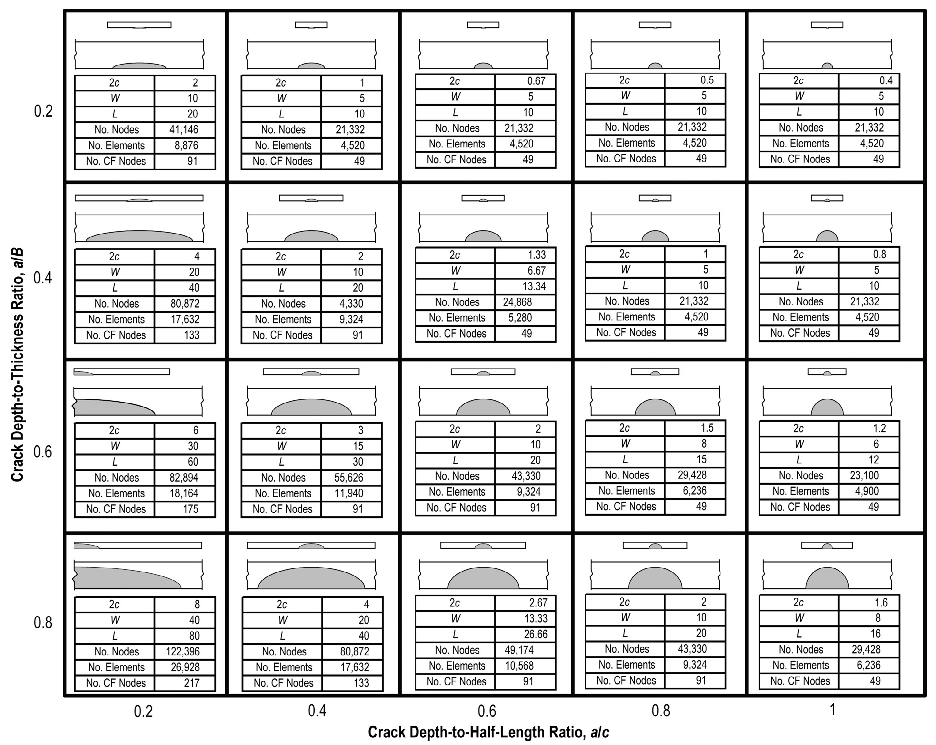
\includegraphics[width=0.8\textwidth]{tasc-geometries}
\caption{20 normalized geometries:\\ \(0.2 \leq \frac{a}{c} \leq 1.0,\; 0.2 \leq \frac{a}{t} \leq 0.8\)}
\end{figure}
\end{column}
\begin{column}{0.45\textwidth}
\begin{figure}
\centering
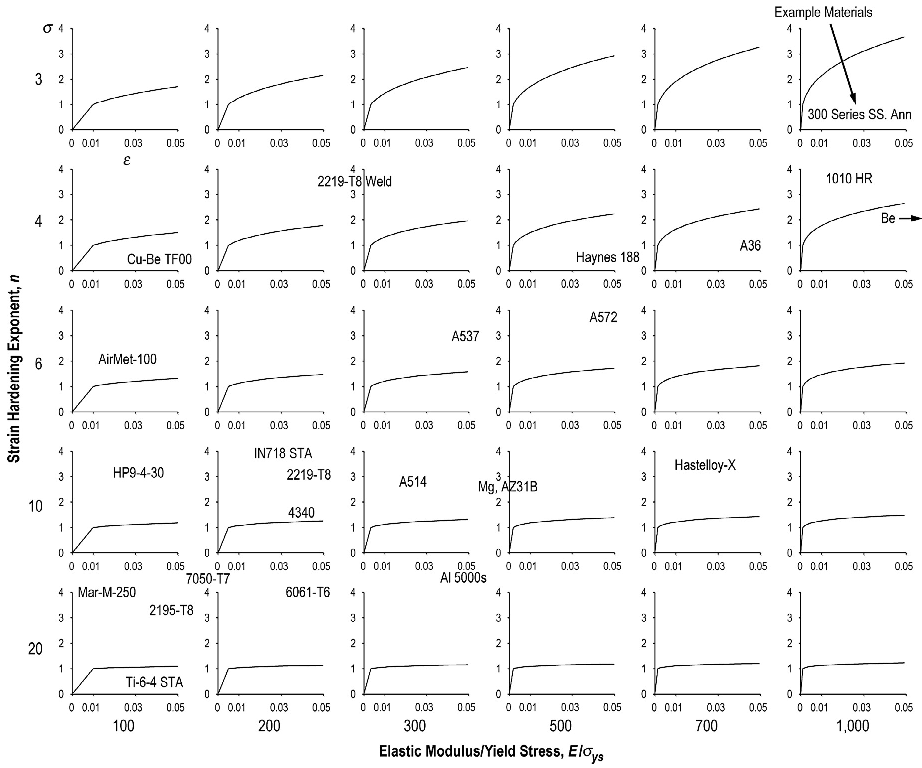
\includegraphics[width=0.8\textwidth]{tasc-materials}
\caption{30 normalized materials:\\ \(100 \leq \frac{E}{S_{\text{ys}}} \leq 1000,\; 3 \leq n \leq 20\)}
\end{figure}
\end{column}
\end{columns}
\note{
But in 2014, Phillip Allen at NASA released TASC, the tool for analysis of surface cracks.
\vfill
TASC includes elastic-plastic results from 600 finite element analyses: all combinations of 20 normalized geometries and 30 normalized materials shown here.
\vfill
It interpolates results for intermediate values, but only includes models for plates in tension.
\vfill
No bending results are included, so work remained on satisfying the entire E2899 standard.
\vfill
}
\end{frame}

\section{Verification and Validation}

\begin{frame}
\begin{columns}
\begin{column}{0.45\textwidth}
\begin{itemize}
\item Analytical and experimental methods both have inherent uncertainty
\item Differences between predicted and measured behavior stem from two main causes:
\begin{itemize}
\item repeatability and accuracy of measurements or calculations
\item using the correct models or procedures to include all significant physical effects
\end{itemize}
\end{itemize}
\end{column}
\begin{column}{0.45\textwidth}
\begin{itemize}
\item First cause is resolved by performing {\bfseries verification} tests (building the product right)
\item Second cause is resolved by performing {\bfseries validation} tests (building the right product)
\end{itemize}
\end{column}
\end{columns}
\note{%
We always want our models or experiments to predict real-world behavior as closely as possible.
\vfill
But there's always going to be some uncertainty and differences between the prediction and the actual behavior.
\vfill
The root cause of differences can generally be lumped into one of two categories:
\vfill
Either a measurement or calculation has limited repeatability or accuracy,
\vfill
or we aren't using the right model or right procedure to include all the relevant physical effects.
\vfill
Fixing problems with repeatability or accuracy is improving verification,
\vfill
and fixing problems with selecting the right models and procedures is improving validation.
\vfill
}
\end{frame}

\begin{frame}
Some V\&V studies include:
\begin{itemize}
\item \citet{favanesi1994} comparing predictions from the NASCRAC software against FLAGRO and FRANC2D, and also against others' and their own experimental data
\item \citet{wilson1995} identified problems with both NASCRAC and FLAGRO, including fracture properties that were treated as constants instead of functions of geometry and load
\item \citet{mcclung2012} verified a \K solution by comparing the FADD3D, FEACrack, and FLAGRO solvers---all were similar except for FEACrack at \(\phi=0\) and \(\phi=\pi\)
\end{itemize}
\note{
Some of the literature on verification and validation includes \citet{favanesi1994} who checked NASCRAC against FLAGRO, FRANC2D, plus a range of experimental data,
\vfill
\citet{wilson1995} identifying errors in NASCRAC and FLAGRO,
\vfill
and \citet{mcclung2012} verifying a \K solution among FADD3D, FEACrack, and FLAGRO, and finding some anomalies at the free surface with FEACrack.
\vfill
}
\end{frame}

\part{Modeling Preparation for Research Tasks%
\note{Time check: 10--12 minutes here.
\vfill
It made sense to develop my modeling techniques for surface cracks in bending on existing results, and that's what's shown in this part.\vfill}%
}

\section{EPRI \hone Verification}

\begin{frame}
\begin{columns}
\begin{column}{0.45\textwidth}
\begin{figure}[tbp]
    \centering
    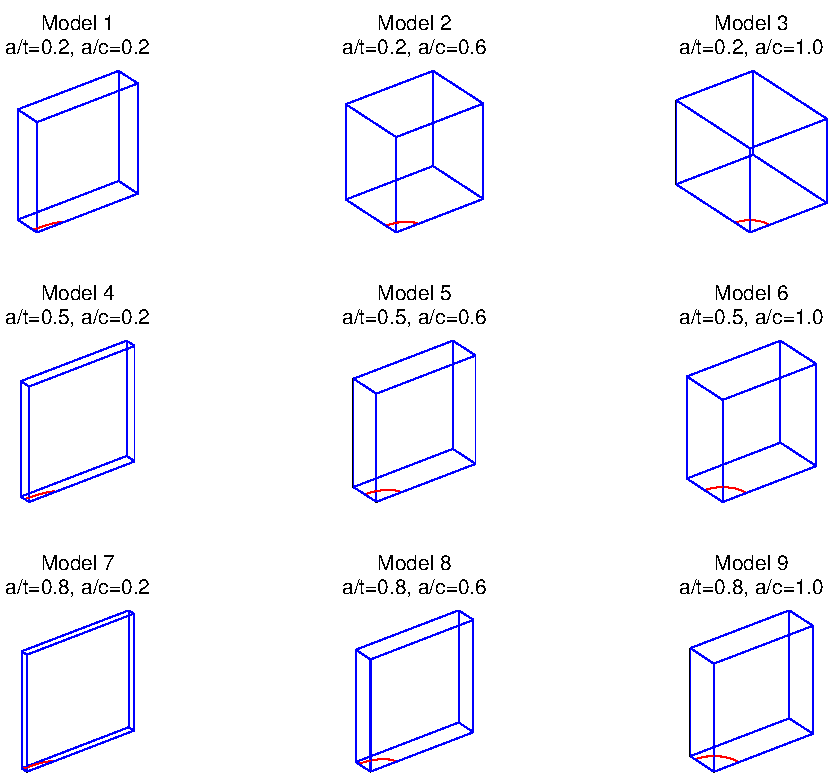
\includegraphics[width=0.8\columnwidth]{geometries}
    \caption{McClung et al. model geometry}
\end{figure}
\end{column}
\begin{column}{0.45\textwidth}
\begin{align*}
\hone &= \frac{\Jpl}{\alpha \sigma_0 \epsilon_0 t \left( \frac{\sigma}{\sigma_0}\right)^{n+1}}
\end{align*}
\begin{figure}
  \centering
  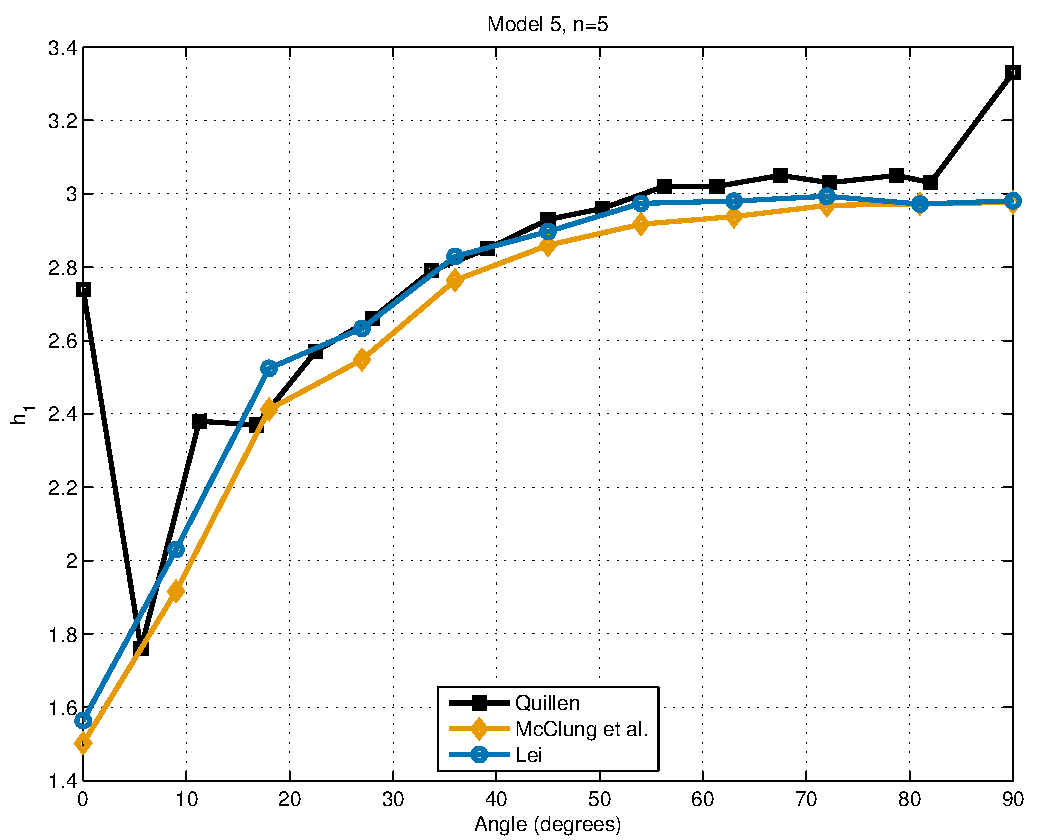
\includegraphics[width=0.7\columnwidth]{model5_n5}
\end{figure}
\end{column}
\end{columns}
\note{
I started at first with EPRI \hone estimates for plates in tension.
\vfill
This spans the same range of crack geometries as TASC, and followed the M.S. research for Eric Quillen, where his results consistently showed some odd anomalies in \J and \hone values at three locations along the crack front.
\vfill
At the time, it was simplest to reconstruct Eric's models in a newer version of Abaqus using Python to create the models, and all the anomalous \hone results disappeared.
\vfill
I wasn't sure if the root cause of the anomalies was the version of Abaqus or something in Eric's input files.
\vfill
But I did have improved methods for building reproducible FEA models by writing Python scripts instead of constructing purpose-built models interactively.
\vfill
}
\end{frame}

\section{Load Separation Verification}

\begin{frame}
\begin{columns}
\begin{column}{0.45\textwidth}
\begin{figure}[tbp]
\centering
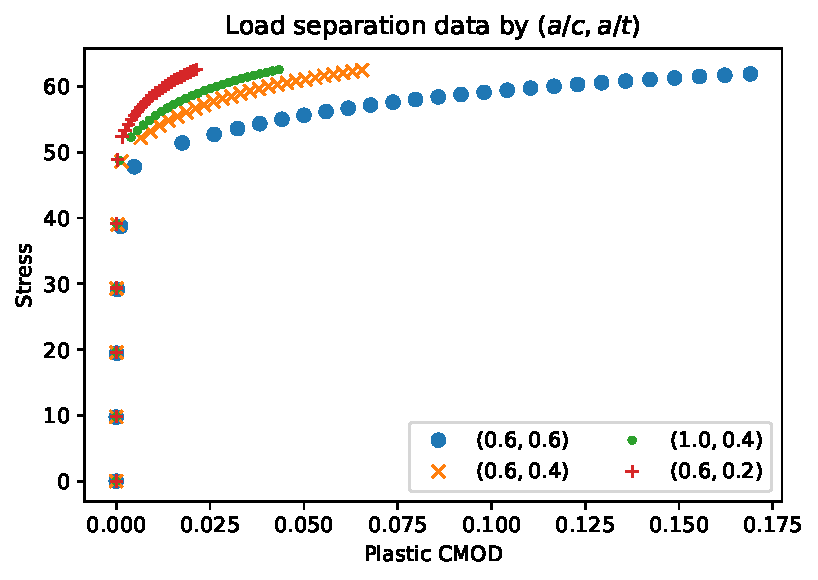
\includegraphics[width=\textwidth]{loadsep-stress-cmodpl-tension}
\caption{Tensile stress versus plastic CMOD}
\end{figure}
\end{column}
\begin{column}{0.45\textwidth}
\begin{figure}[tbp]
\centering
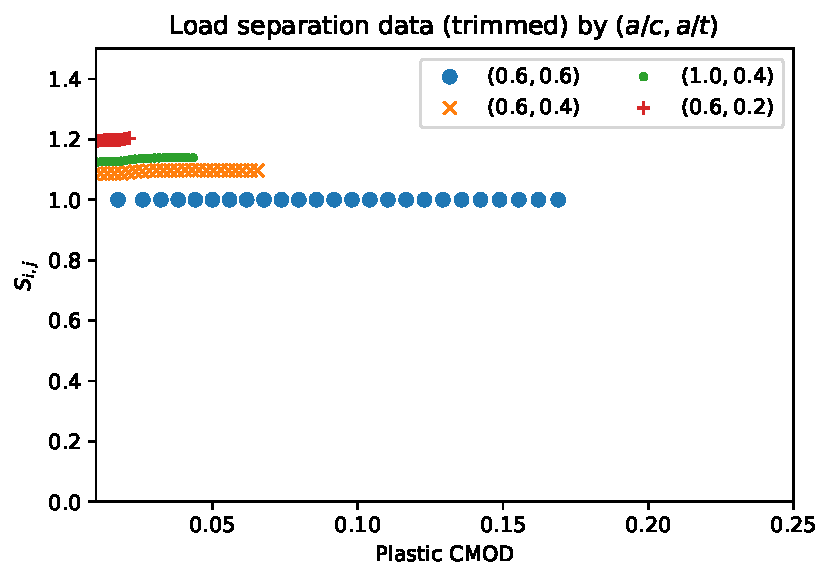
\includegraphics[width=\textwidth]{cmodpl_Sij_tension}
\caption{\label{fig:sij_cmodpl} Separation parameter values versus plastic CMOD}
\end{figure}
\end{column}
\end{columns}
\note{
More recently, I adapted a few TASC geometries similar to those used by Sharobeam and Landes for load separation in surface cracks.
\vfill
The left graph shows the stress versus the plastic component of CMOD.
\vfill
Taking the most compliant model as the reference curve, the graph on the right shows the separation parameters calculated from dividing each curve by the reference curve,
\vfill
and they show the constant values expected from having enough plastic deformation in the models
\vfill
}
\end{frame}

\begin{frame}
\begin{center}\(
\frac{b_e}{t} = 1 - \frac{\pi a}{2t \left[ 2 + \frac{a/c}{a/t} \right]}
\)\end{center}
\begin{columns}[t]
\begin{column}{0.45\textwidth}
\begin{figure}[tbp]
\centering
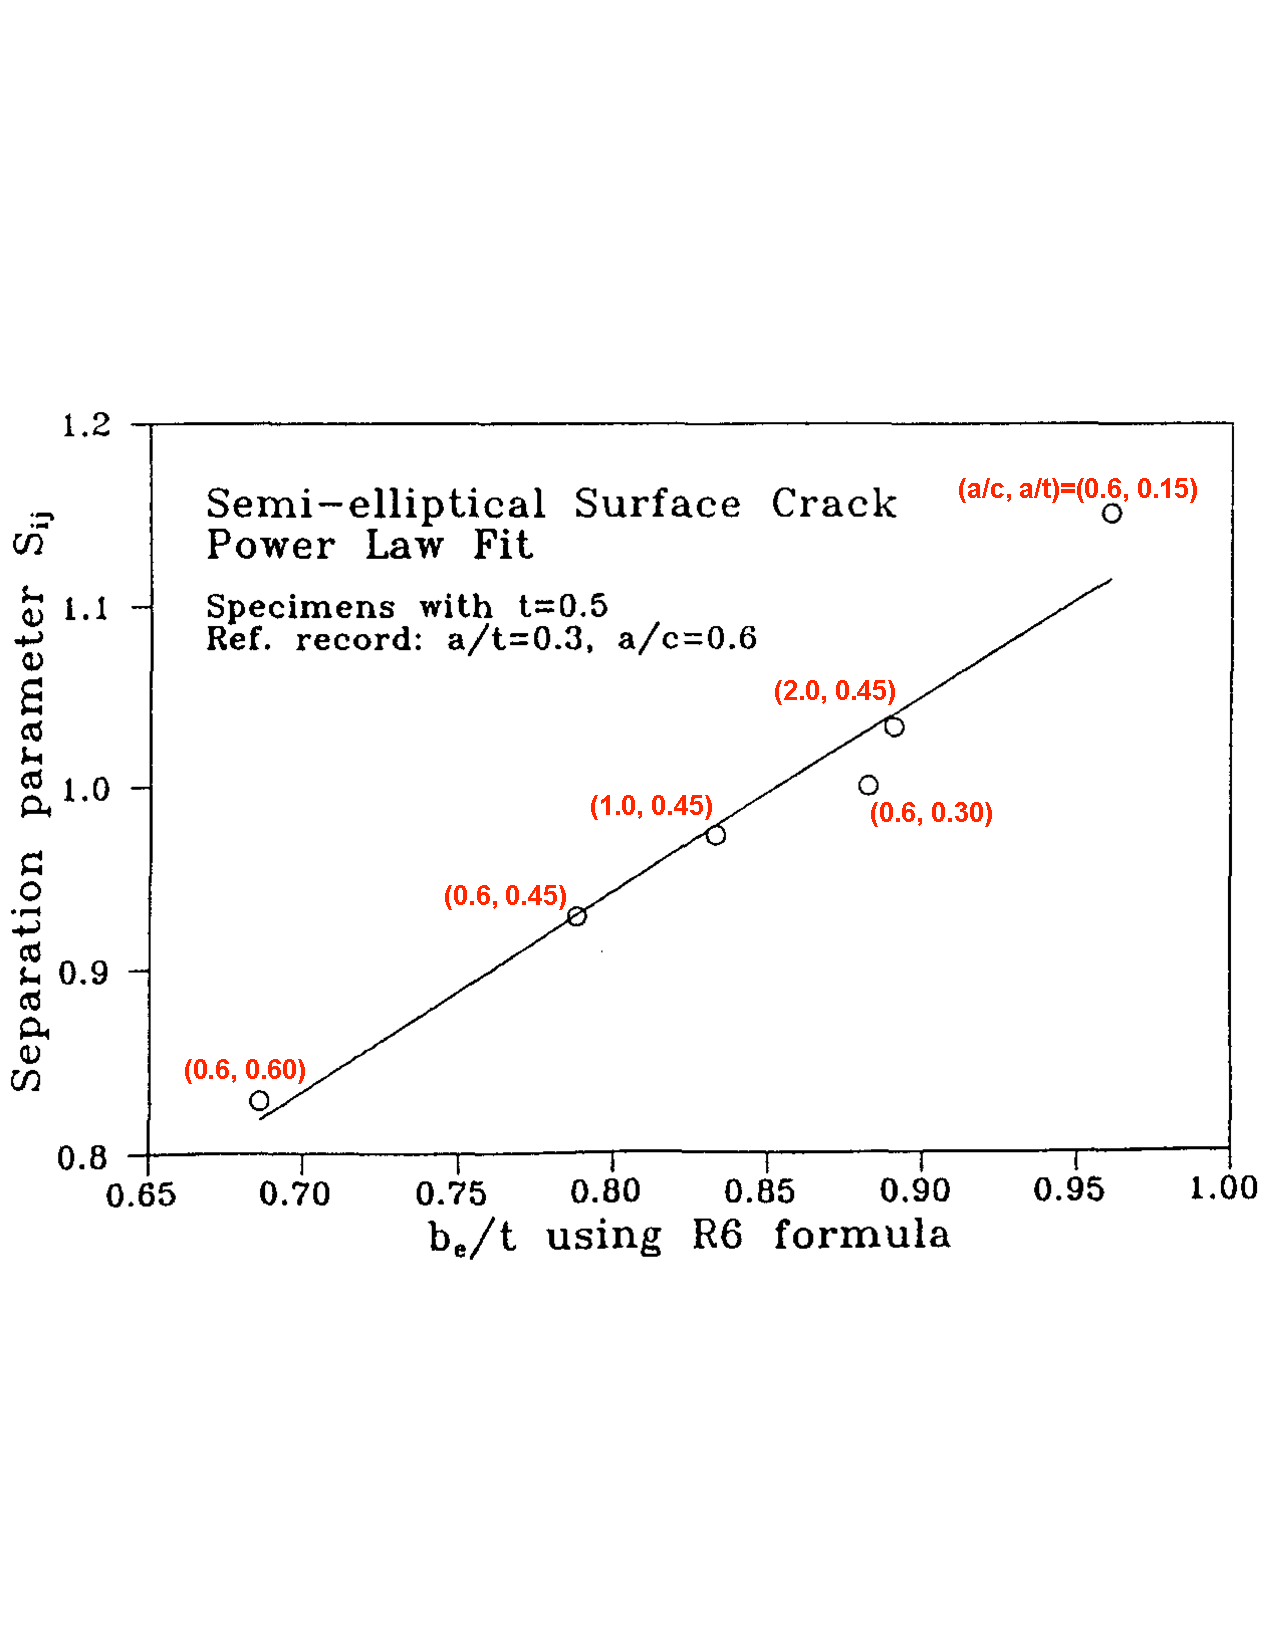
\includegraphics[width=0.9\textwidth]{load-sep-tension-sl-2}
\caption{\label{fig:load-sep-tension-sl} Annotated from \cite{sharobeamlandes1993}}
\end{figure}
\end{column}
\begin{column}{0.45\textwidth}
\begin{figure}[tbp]
\centering
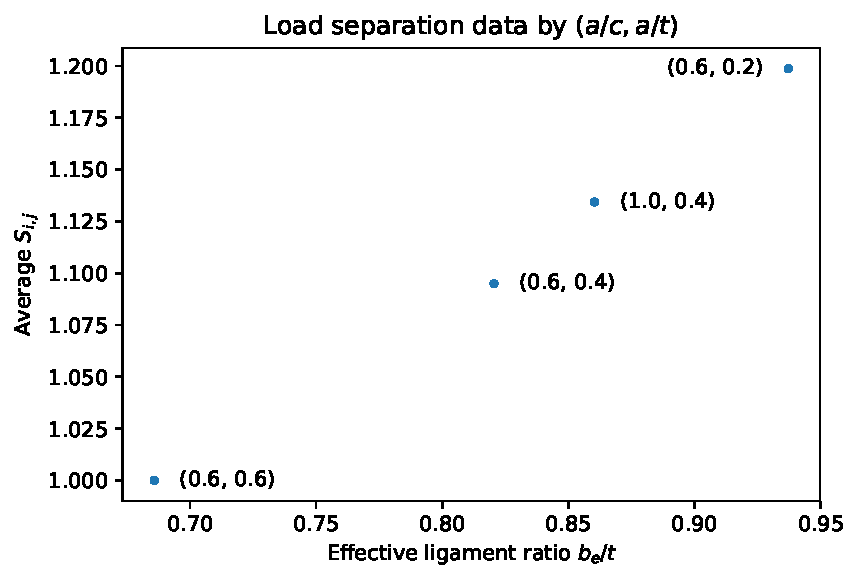
\includegraphics[width=0.9\textwidth]{bet_Sij_tension}
\caption{\label{fig:load-sep-tension-mwr} From current work}
\end{figure}
\end{column}
\end{columns}
\note{
Plotting the separation parameters against the effective length of the uncracked ligament, the results on the right figure lie near a linear fit similar to the one in the left figure.
\vfill
}
\end{frame}

\section{Verification of Two TASC Cases}

\subsection{Applying Procedure to a New Material Model (\(\frac{E}{\Sys}=150\))}

\begin{frame}
\begin{figure}[tbp]
\centering
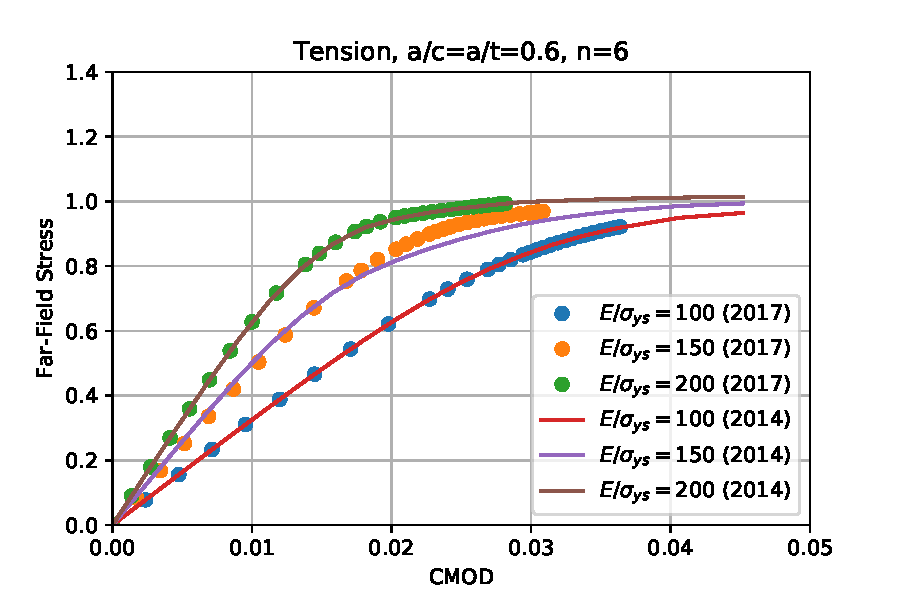
\includegraphics[width=0.6\columnwidth]{e100_150_200_verification}
\caption{\label{fig:e100_150_200_verification} Comparison of normalized FEA results, interpolated result, and TASC raw data}
\end{figure}
\note{
Then I moved on to digging into the internals of the TASC model database,
\vfill
seeing if I could make models that would match two of the ones from the database,
\vfill
and a third model to test the limits of the interpolation method.
\vfill
On this figure, the lines represent TASC results for \(E=100\) and \(E=200\), with an interpolated result for \(E=150\).
\vfill
The circles represent my model results at each modulus, and you can see that the results are identical for \(E=100\) and \(E=200\), and that the interpolated TASC result is a few percent more compliant than the actual results from the same modulus.
\vfill
}
\end{frame}

\part{Research Plan for Bending Models and Modified TASC Program%
\note{Time check: be at the 15--17 minute mark here.
\vfill
So now we get to the plan for the new research work\vfill}
}

\section{Creating Plate Models}

\begin{frame}
\begin{center}
\(t = 1 \quad 0.2 \leq \frac{a}{c} \leq 1.0 \quad 0.2 \leq \frac{a}{t} \leq 0.8\) \\
\(W = 5 \max(c, t) \quad \Sinner = W \quad \Souter = 2W \quad L = 1.1 \Souter\)
\end{center}
\begin{columns}
\begin{column}{0.45\textwidth}
\begin{figure}
\centering
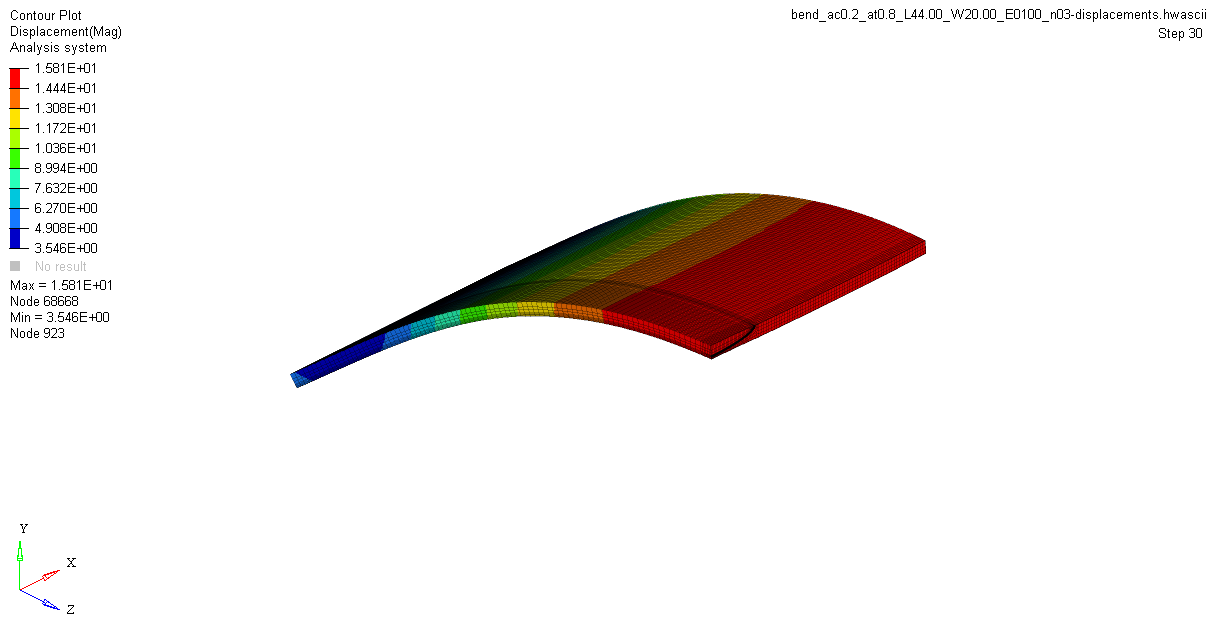
\includegraphics[width=\columnwidth]{bend_ac02_at08_E0100_n03}
\caption{\label{fig:bend_ac02_at08_E0100_n03} Plate model, \(\frac{a}{c}=0.2\), \(\frac{a}{t}=0.8\)}
\end{figure}
\end{column}
\begin{column}{0.45\textwidth}
\begin{figure}
\centering
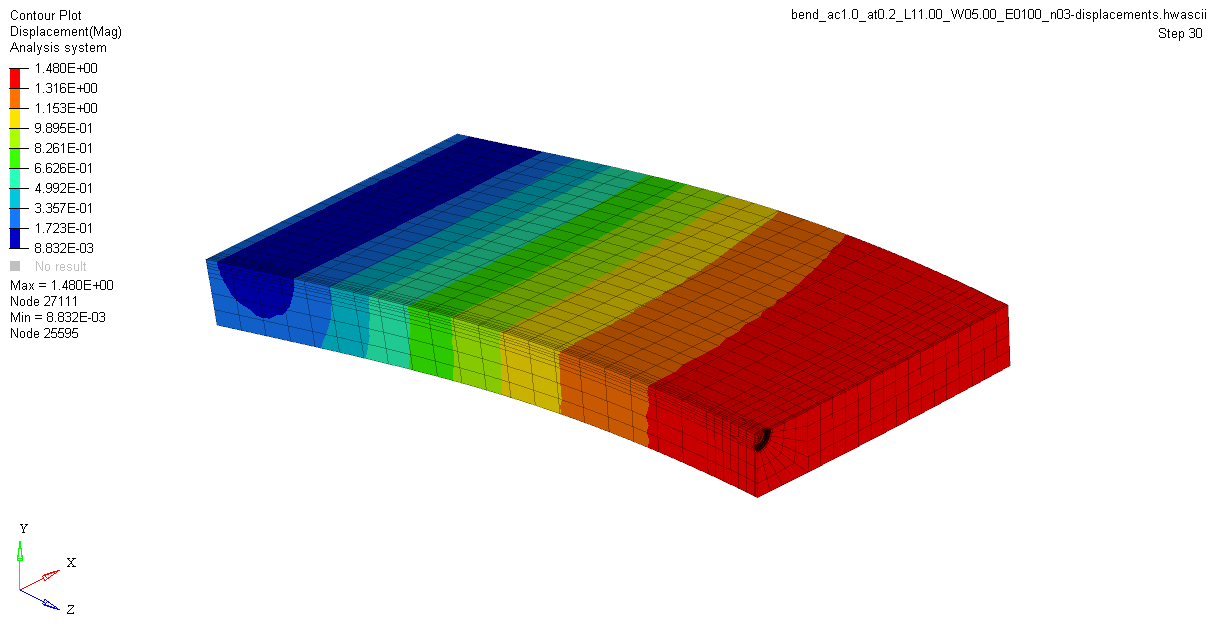
\includegraphics[width=\columnwidth]{bend_ac10_at02_E0100_n03}
\caption{\label{fig:bend_ac10_at02_E0100_n03} Plate model, \(\frac{a}{c}=1.0\), \(\frac{a}{t}=0.2\)}
\end{figure}
\end{column}
\end{columns}
\note{
The dimensions on each plate follow the same rules.
\vfill
Each model represents 1/4 of the full experimental plate, and has thickness of 1 inch.
\vfill
Model width is 5 times larger than either the crack half width or the plate thickness, whichever is larger.
\vfill
The plane where the inner rollers would appear will be a distance W from the center, and the line representing the outer rollers will be spaced at twice that distance.
\vfill
The whole plate will extent 10\% past the outer roller location.
\vfill
All these models will start from a single input file for the FEACrack program, and a Python script will run FEACrack with command-line parameters to adjust dimensions and write a new input file for WARP3D for each of 20 geometries.
\vfill
After that, the same Python script can adjust material properties in the 20 WARP3D input files and write a new input file for each of 30 materials.
\vfill
}
\end{frame}

\section{Solving Plate Models, Optimizing Boundary Conditions}

\begin{frame}
\citet{allenwells2014} reported \(M = \frac{r_{\phi} \Sys}{\J} < 25\) for tension

\begin{columns}
\begin{column}{0.45\textwidth}
\begin{figure}[tbp]
\centering
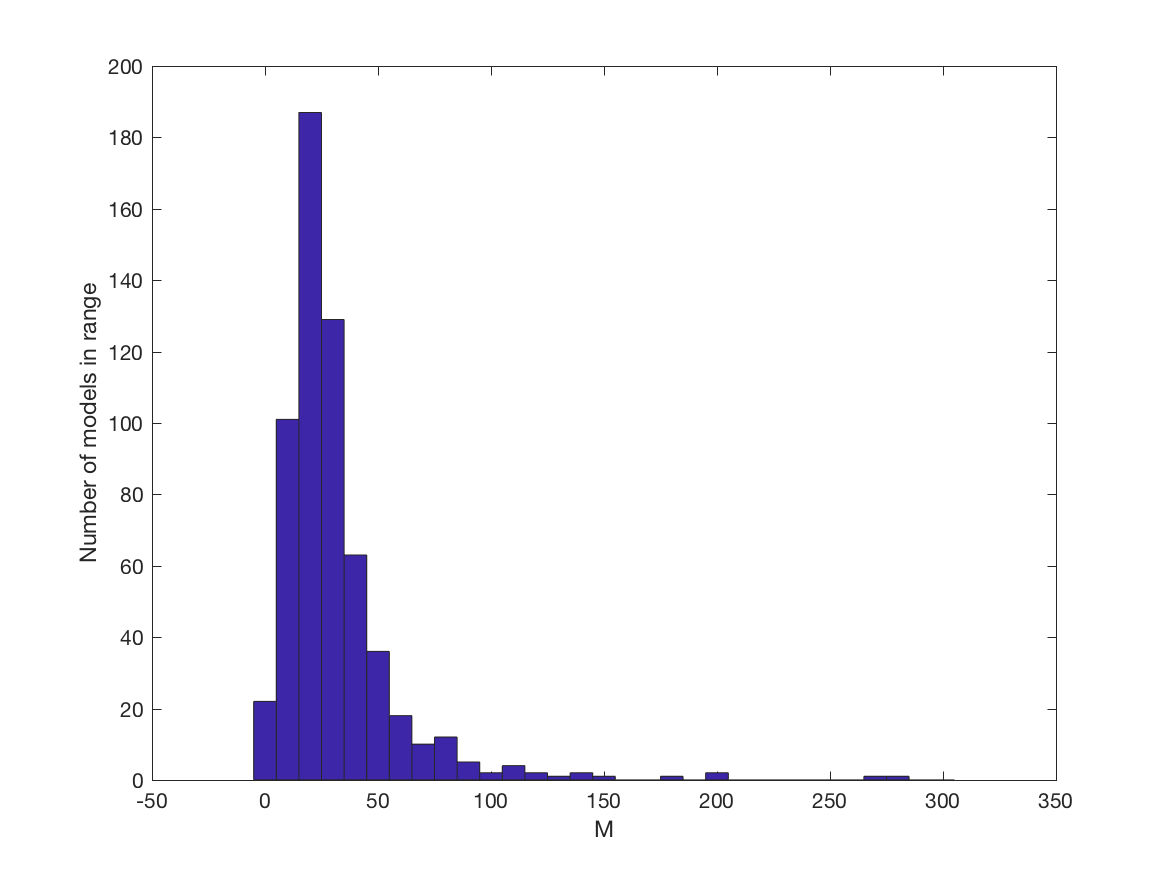
\includegraphics[width=0.7\columnwidth]{min_M_hist}
\caption{Histogram of \(M\) results from TASC tension model database}
\end{figure}
\end{column}
\begin{column}{0.45\textwidth}
\begin{figure}[tbp]
\centering
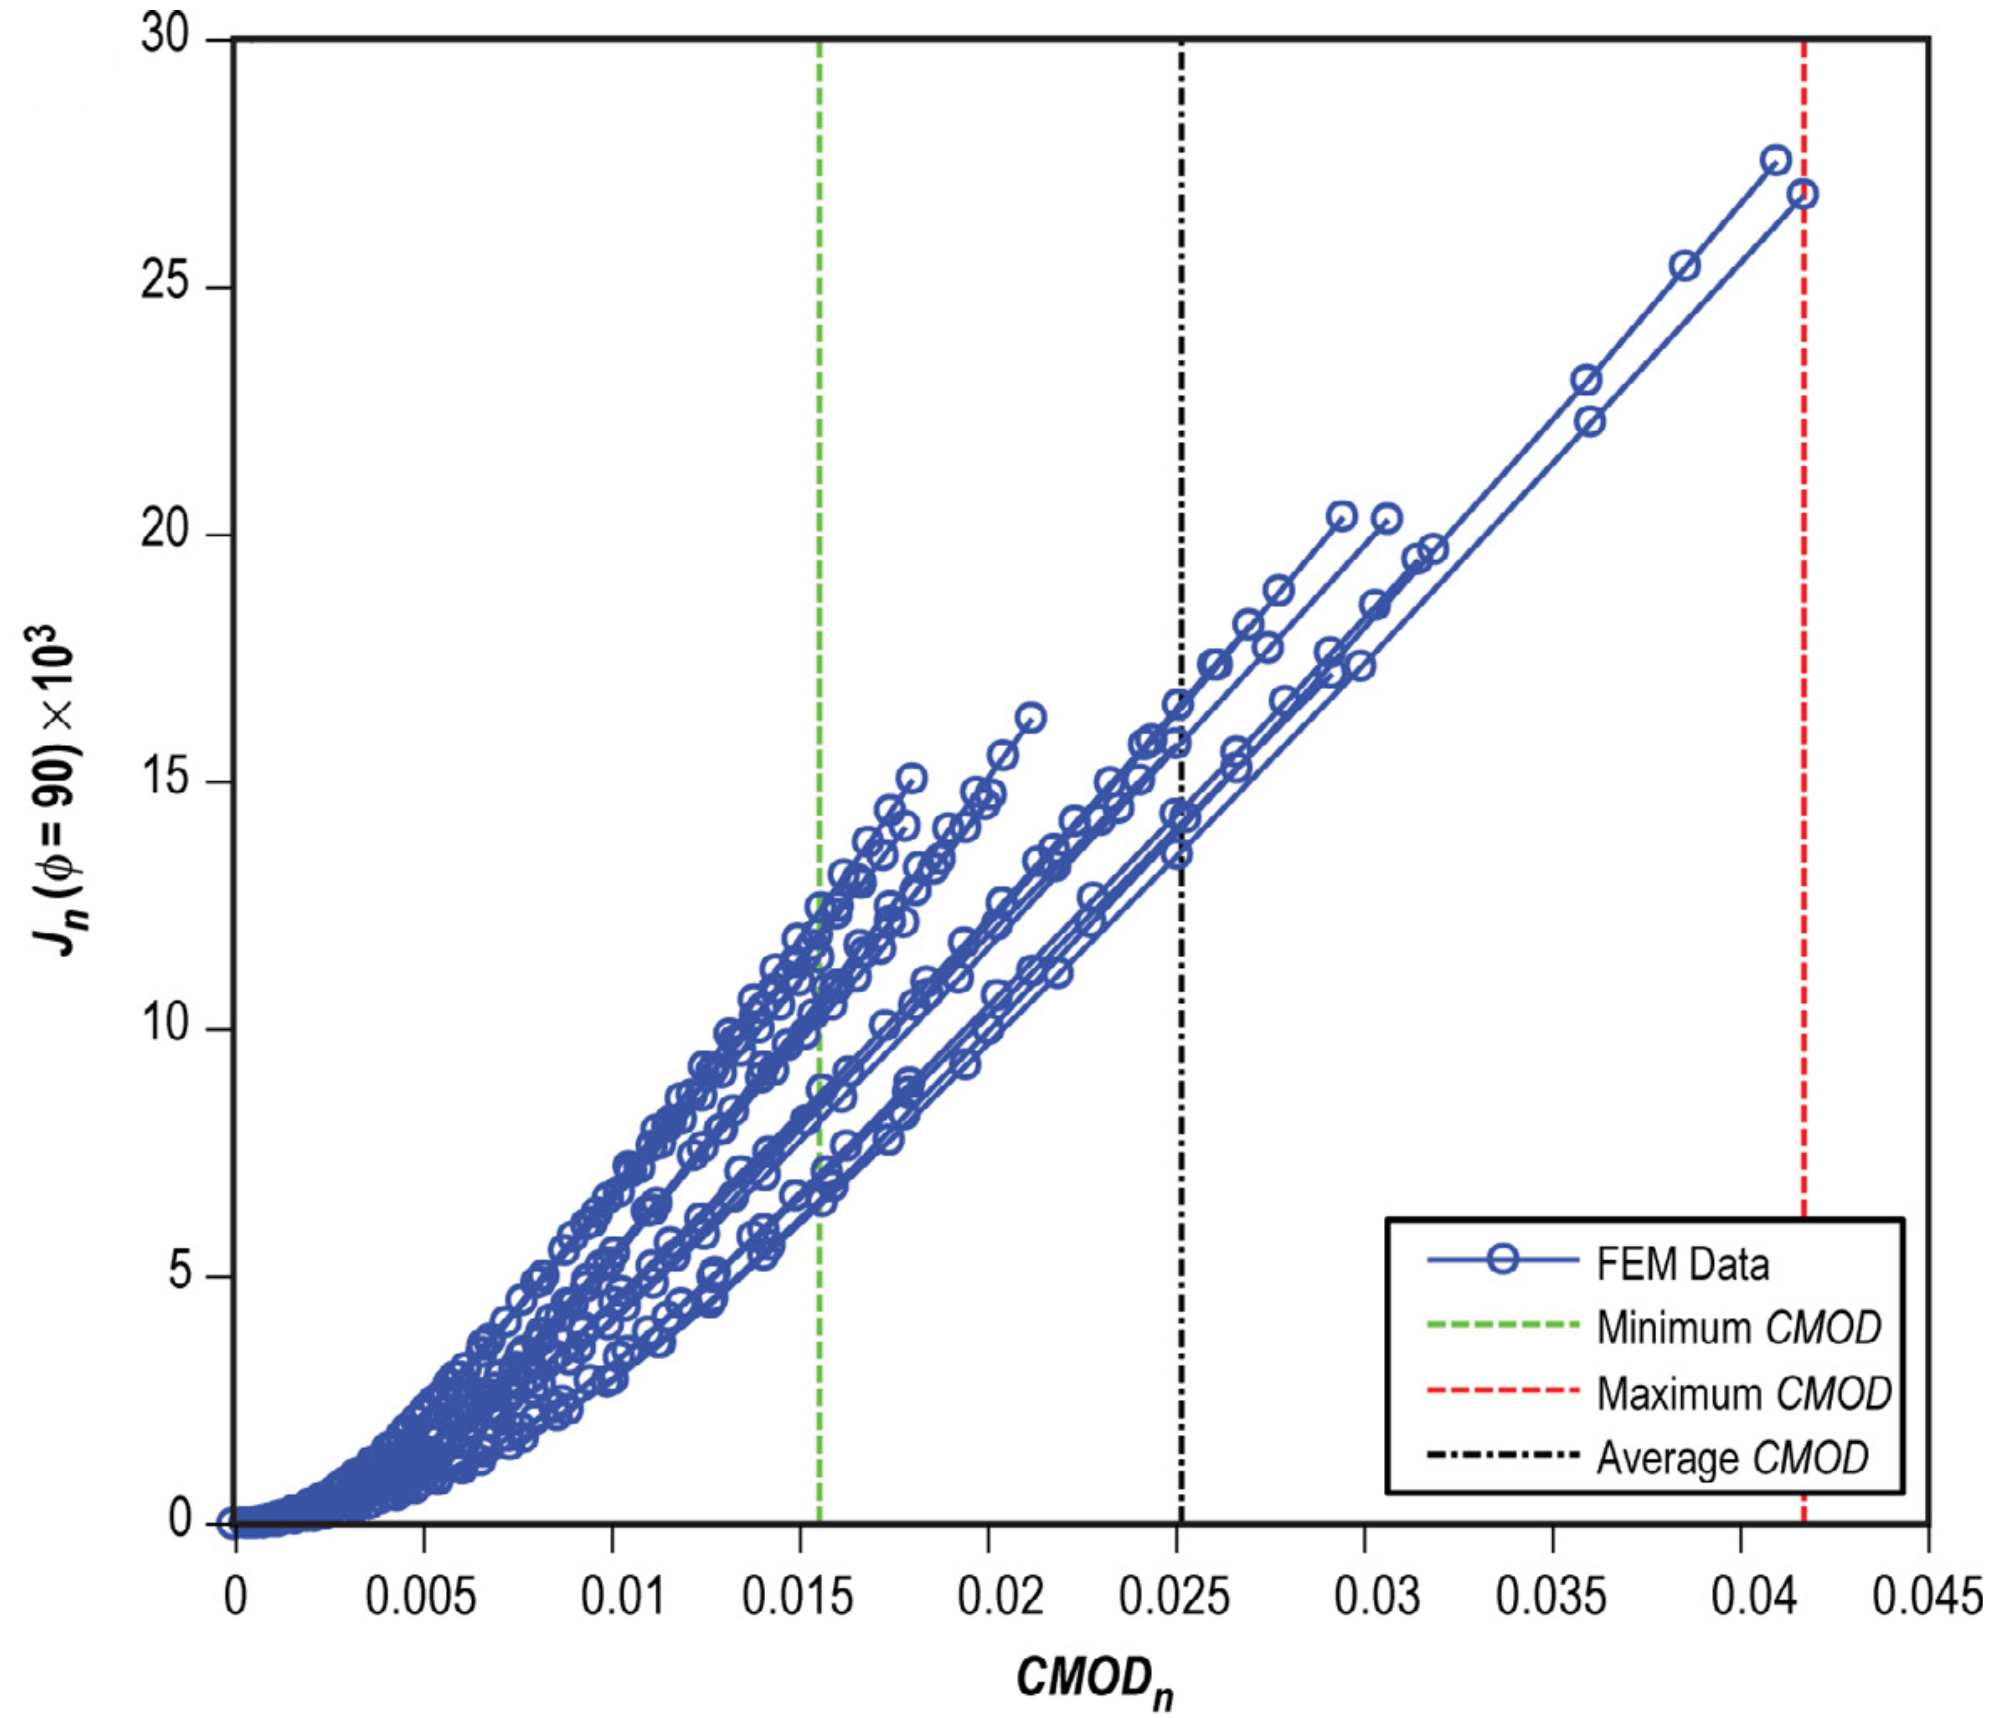
\includegraphics[width=0.7\columnwidth]{J-CMOD-extrapolation}
\caption{\J-CMOD graph used for extrapolation}
\end{figure}
\end{column}
\end{columns}
\note{
The TASC literature indicated models were loaded until \J values were high enough to drive this dimensionless deformation formula below 25,
\vfill
but looking at the full set of M values recorded in the TASC database shown in the left figure, it's clear many of the models didn't reach that deformation level.
\vfill
The real criteria for loading is to load the model heavily enough to straighten the \J-CMOD curves shown in the right figure so we can accurately extrapolate beyond the applied load.
\vfill
}
\end{frame}

\begin{frame}
\begin{columns}
\begin{column}{0.45\textwidth}
\begin{figure}[tbp]
\centering
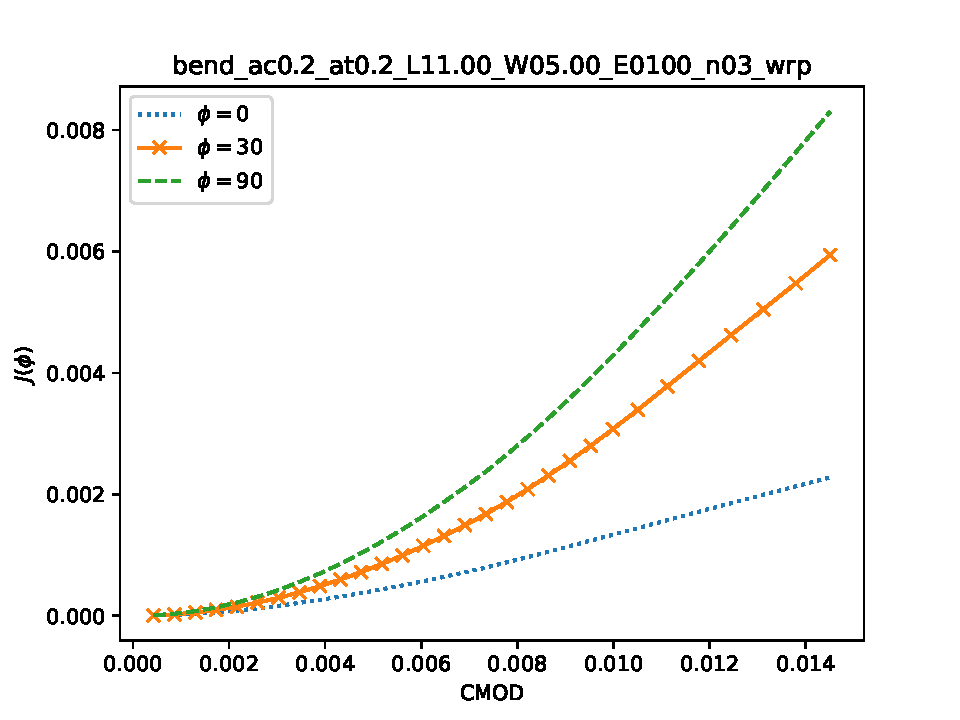
\includegraphics[width=0.9\columnwidth]{J_CMOD_bend_ac02_at02_L1100_W0500_E0100_n03_wrp}
\caption{\(\frac{a}{c}=0.2\), \(\frac{a}{t}=0.2\), \(E=100\), \(n=3\)}
\end{figure}
\end{column}
\begin{column}{0.45\textwidth}
Adjust boundary conditions until
\begin{itemize}
\item slope of last 20\% of \J-CMOD curve is \(20\times\) larger than initial slope
\item slope of last 20\% of \J-CMOD curve is \(<10\%\) different than slope of previous 20\%
\end{itemize}
at \(\phi=\) \SI{30}{\SIUnitSymbolDegree}
\end{column}
\end{columns}
\note{
As a result, since we have a full set of \J-\(\phi\)-CMOD data after running a model, my plan was to increase loads until the two criteria shown here were met at \(\phi=\) \SI{30}{\SIUnitSymbolDegree}.
\vfill
This ensures that the last 40\% of the \J-CMOD curve is consistently straight, and any major curvature is confined to the first 60\% of the range.
\vfill
}
\end{frame}

\begin{frame}
Displacement control for tension models makes optimization easier
\begin{columns}[t]
\begin{column}{0.45\textwidth}
\begin{figure}[tbp]
\centering
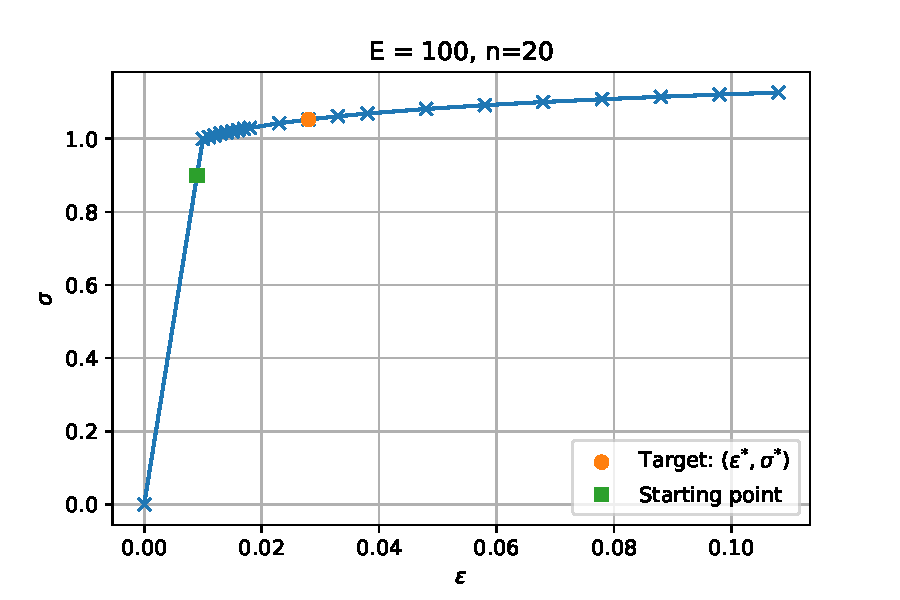
\includegraphics[width=0.9\columnwidth]{secant-1}
\caption{\label{fig:secant-1}Example stress-strain curve using linear plus power law (LPPL) formulation}
\end{figure}
\end{column}
\begin{column}{0.45\textwidth}
\begin{figure}[tbp]
\centering
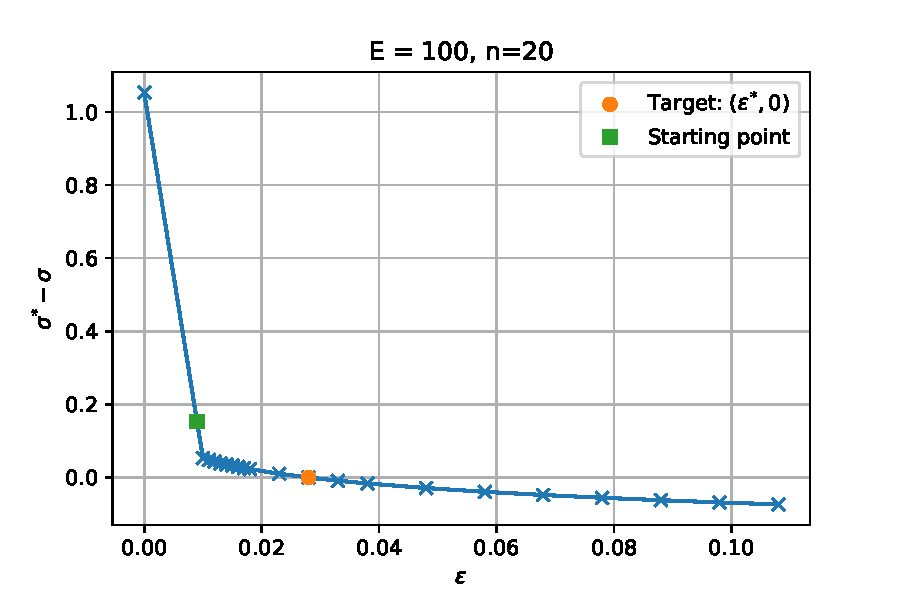
\includegraphics[width=0.9\columnwidth]{secant-2}
\caption{\label{fig:secant-2}Transformed to find required strain level}
\end{figure}
\end{column}
\end{columns}
\note{
Early versions of satisfying this load criteria for tension models used displacement boundary conditions, and some convenient optimizations could take place.
\vfill
Because we're effectively adjusting strain to match a target stress, the left stress-strain curve can be transformed to the form on the right, and we can do a secant method to find the strain required to drive the transformed stress value to zero.
\vfill
Just move on a tangent at wherever we are on the transformed curve, and we quickly end up at the desired strain value.
\vfill
}
\end{frame}

\begin{frame}
Load control for bending models makes optimization more difficult
\begin{columns}[t]
\begin{column}{0.45\textwidth}
\begin{figure}[tbp]
\centering
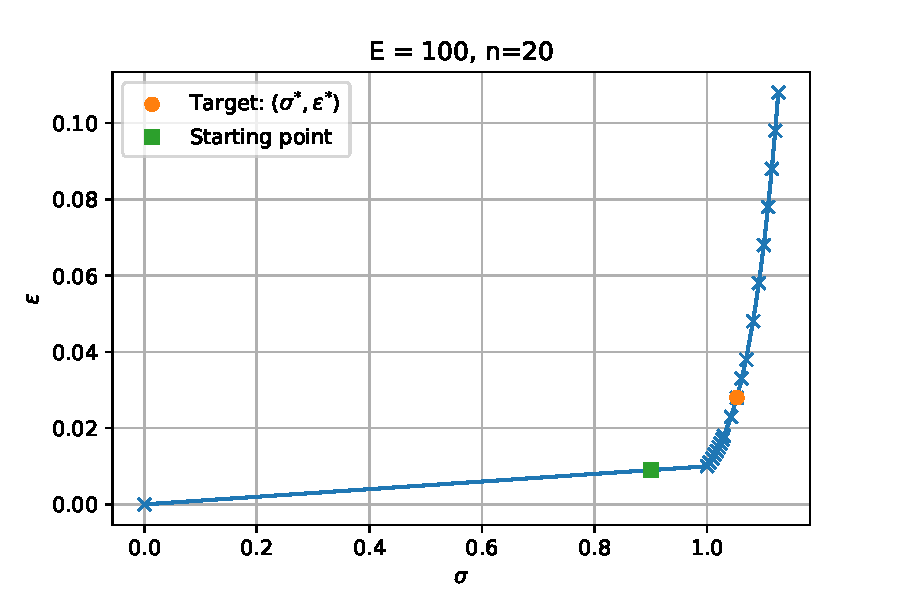
\includegraphics[width=0.9\columnwidth]{secant-3}
\caption{\label{fig:secant-3}Example stress-strain curve using LPPL formulation, transformed to stress-controlled}
\end{figure}
\end{column}
\begin{column}{0.45\textwidth}
\begin{figure}[tbp]
\centering
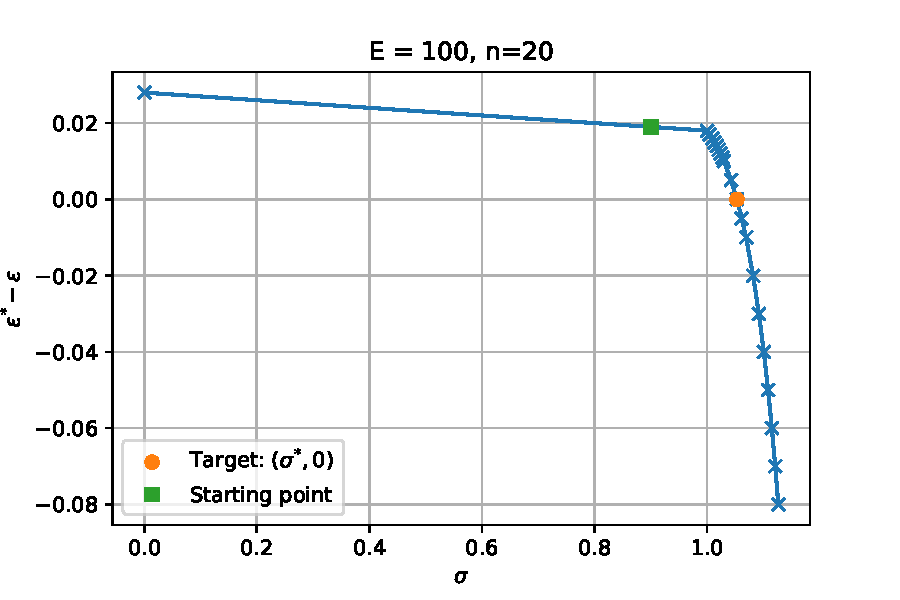
\includegraphics[width=0.9\columnwidth]{secant-4}
\caption{\label{fig:secant-4}Transformed to find required stress level}
\end{figure}
\end{column}
\end{columns}
\note{
Unfortunately, the bending models have to operate with traction boundary conditions, where we effectively adjust applied stress to match a target strain.
\vfill
The secant method won't work, as our first step would run us way off the right side of the transformed graph.
\vfill
So we just have to take small steps and stop whenever we see the curve has straightened out enough.
\vfill
}
\end{frame}

\section{Verification and Validation}

\begin{frame}
\begin{columns}[t]
\begin{column}{0.45\textwidth}
Abaqus validation
\begin{figure}[tbp]
\centering
\includegraphics[width=0.8\columnwidth]{{abq_plate_ac02_at02}}
\caption{\label{fig:abq_plate_ac02_at02} Example Abaqus bending model from FEACrack}
\end{figure}
\end{column}
\begin{column}{0.45\textwidth}
\J convergence
\begin{figure}[tbp]
\centering
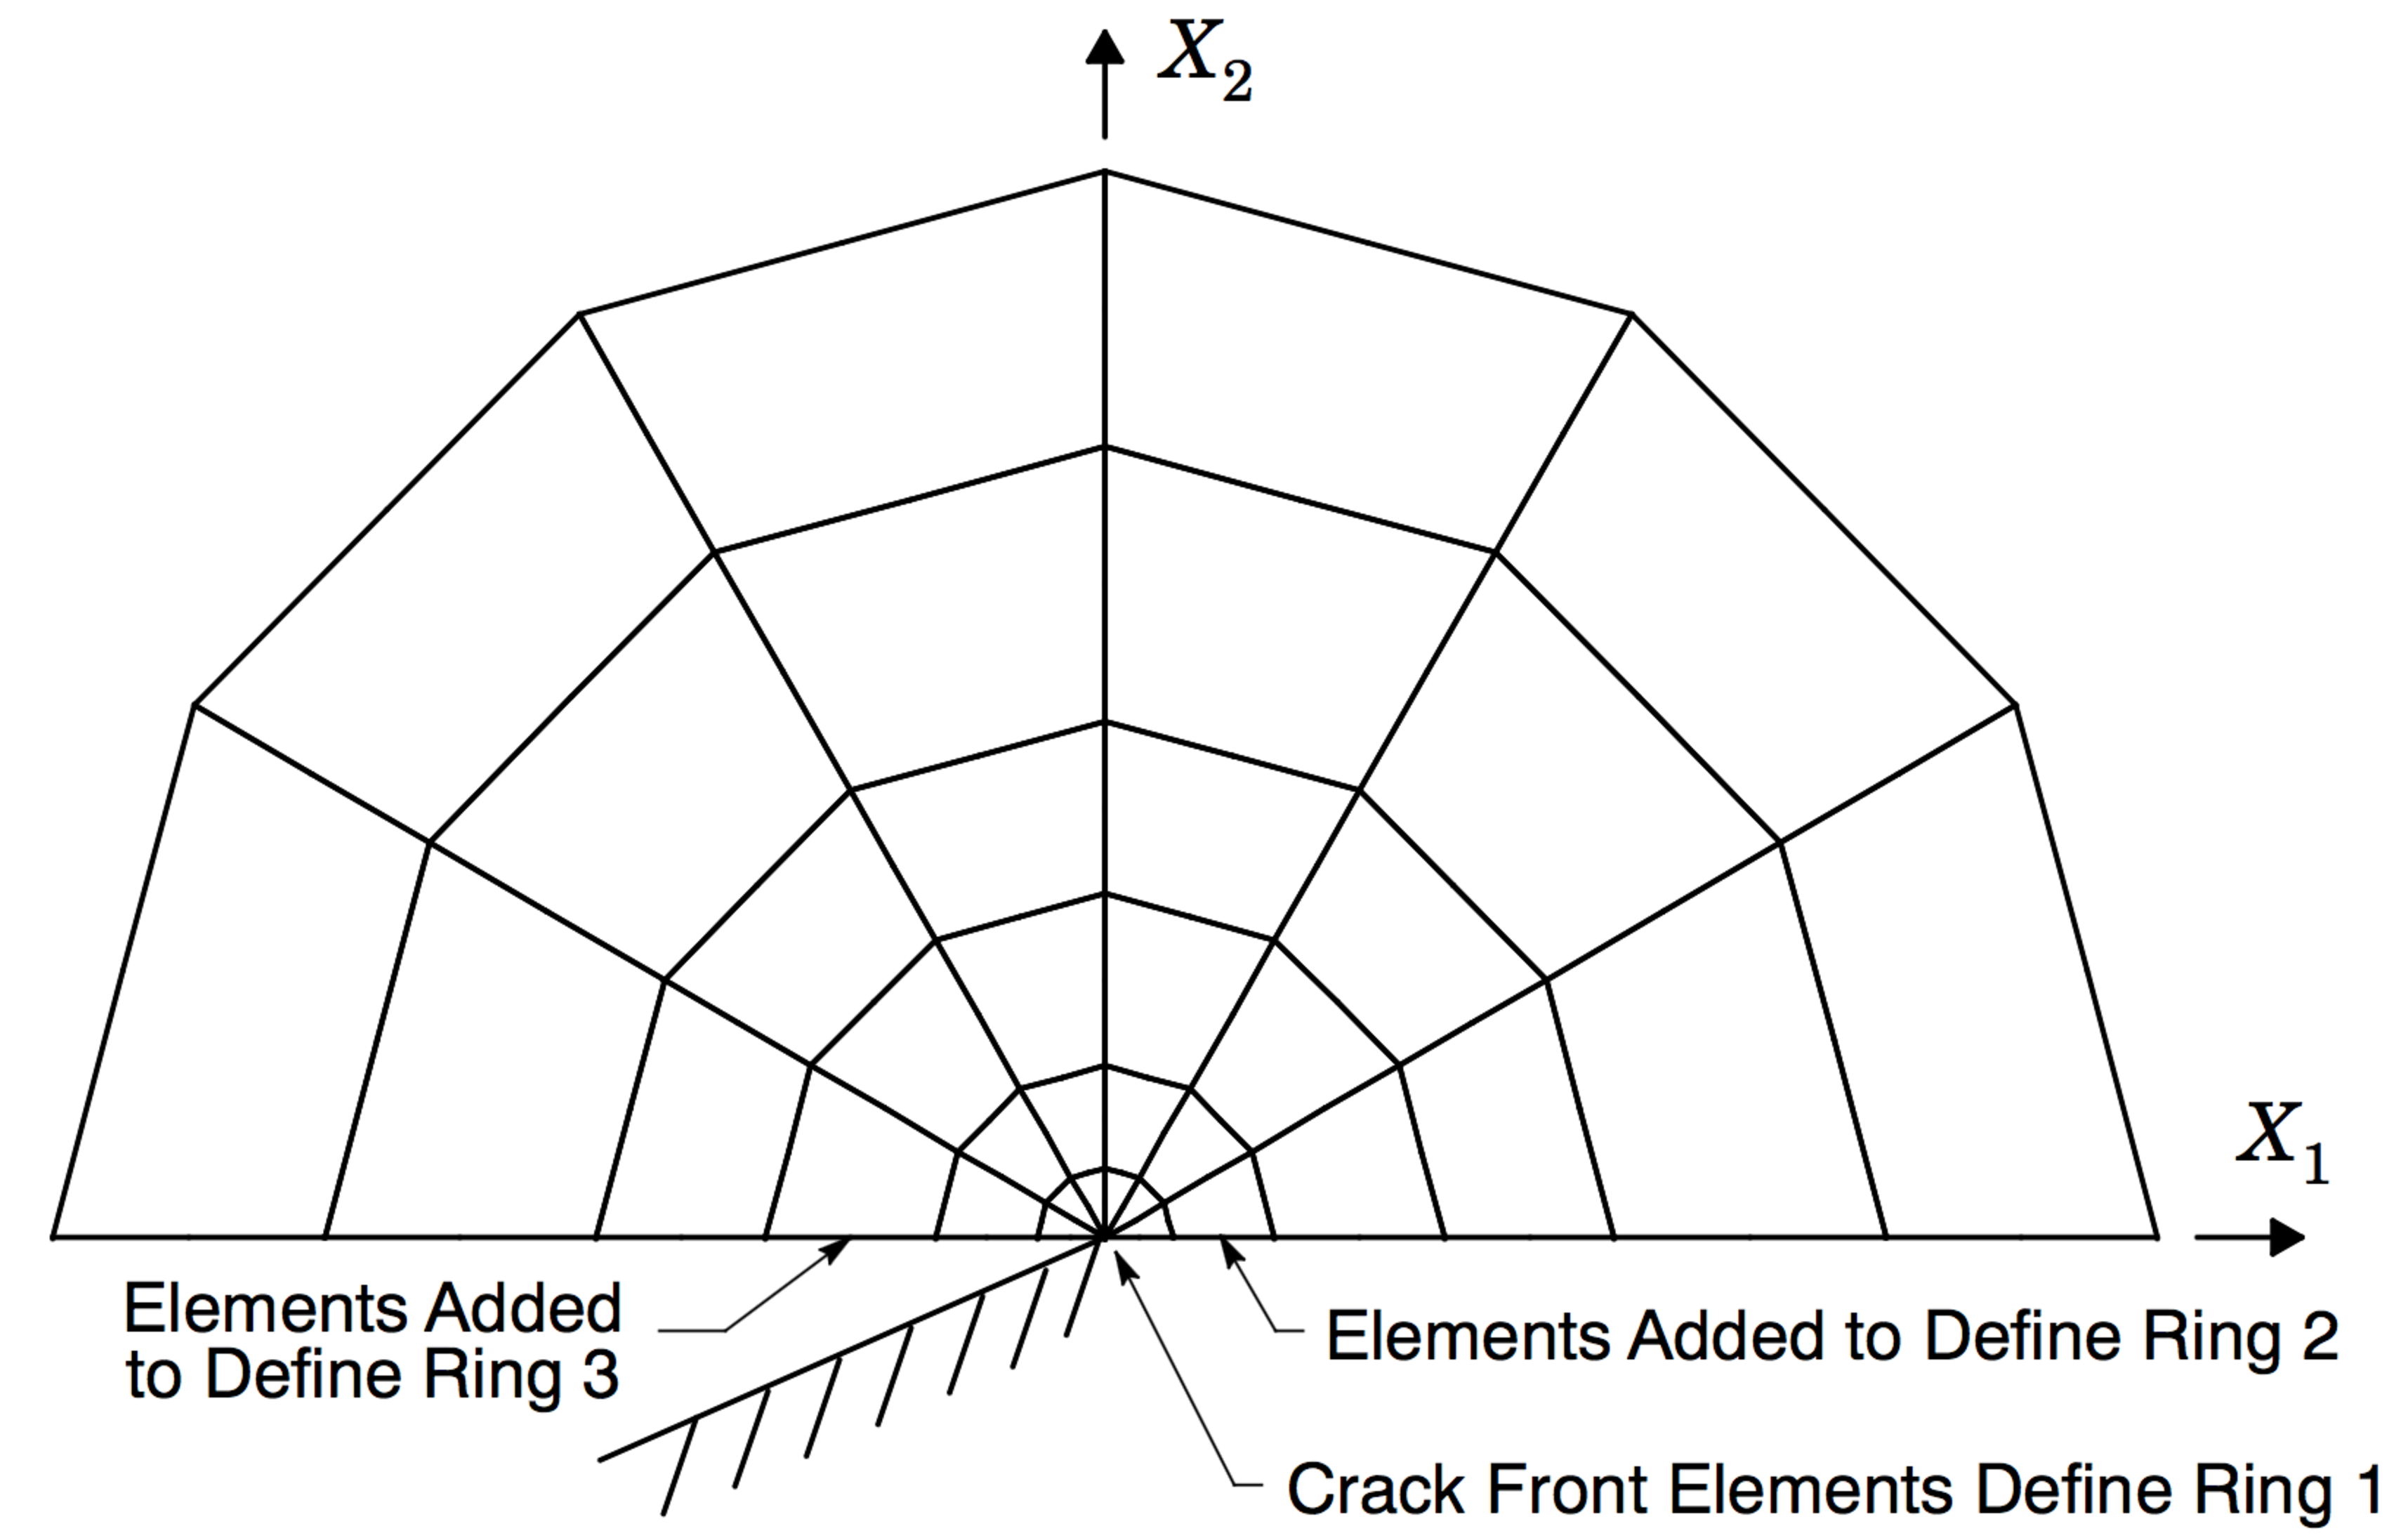
\includegraphics[width=\columnwidth]{contour_integral_regions_warp3d}
\caption{\label{fig:fem-j-domains} Elements used in WARP3D \J calculations}
\end{figure}
\end{column}
\end{columns}
\note{
Since we're going to spend a lot of time finding \J values for the models, it makes sense to do some checks to ensure the \J values are accurate.
\vfill
First, a subset of the models will be run in Abaqus with identical meshes.
\vfill
Second, as \J values can be calculated for any set of elements surrounding the crack front, those \J values should converge to a final result as we add more elements and capture more of the strain energy and work done inside the plastic zone.
\vfill
}
\end{frame}

\section{Updates to TASC}

\begin{frame}[fragile]
\begin{itemize}
\item Don't break anything already working for tension
\item Make a \verb|results_bending| database alongside the existing \verb|results| database for tension
\item Identify any equations only valid for tension models
\item Replace with conditionals checking for model type, then use tension or bending equations as required
\item Interpolation method should need no changes
\item Validate a load-CMOD curve against existing bending experimental data
\end{itemize}
\note{
For modifications to the TASC program, the goal is to make the smallest set of changes required to support bending.
\vfill
We can't break tension results, and most of the code assumes a certain arrangement of data in the database.
\vfill
So we'll make a results\_bending database alongside the existing results database.
\vfill
Any equations that are only applicable for tension will be replaced with a check for which type of analysis we're running, and then picking the right equation
\vfill
There shouldn't need to be any changes to the interpolation parts of TASC
\vfill
and ideally, we'll be able to reproduce an experimental load-CMOD curve from a four-point bend experiment with good accuracy.
\vfill
}
\end{frame}

\section{EPRI \hone Study, Load Separation Study}

\begin{frame}
\begin{columns}[t]
\begin{column}{0.45\textwidth}
EPRI \hone
\begin{itemize}
\item Examine EPRI \hone estimation method
\item Abaqus with fully-plastic check
\item WARP3D results intended for TASC
\end{itemize}
\end{column}
\begin{column}{0.45\textwidth}
Load separation
\begin{itemize}
\item No published literature about load separation for surface cracks in bending
\item Apply load separation to WARP3D results for \(\frac{E}{\Sys}=500, n=4\)
\item Use all 20 geometries for \(0.2 \leq \frac{a}{c} \leq 1.0, 0.2 \leq \frac{a}{t} \leq 0.8\)
\end{itemize}
\end{column}
\end{columns}
\note{
Additionally, I want to do some investigation into both EPRI \hone and load separation.
\vfill
For EPRI, we've got some prior results in the literature for 2D geometries and surface cracks in tension, but not in bending.
\vfill
Same for load separation. Having 20 different crack geometries for each material means I've got plenty of data points for the linear fit.
\vfill
}
\end{frame}

\part{Results and Discussion \note{So how did all of this turn out compared to the original plan?\vfill}}

\section{Improvements to Initial Bending Models}

\subsection{\J Convergence Study}

\begin{frame}
\begin{columns}
\begin{column}{0.45\textwidth}
\begin{figure}[tbp]
\centering
\includegraphics[width=\columnwidth]{{bend_ac02_at08_E0100_n20_wrp_J_converge_abs}}
\caption{Convergence of \J across 10 domains}
\end{figure}
\end{column}
\begin{column}{0.45\textwidth}
\begin{figure}[tbp]
\centering
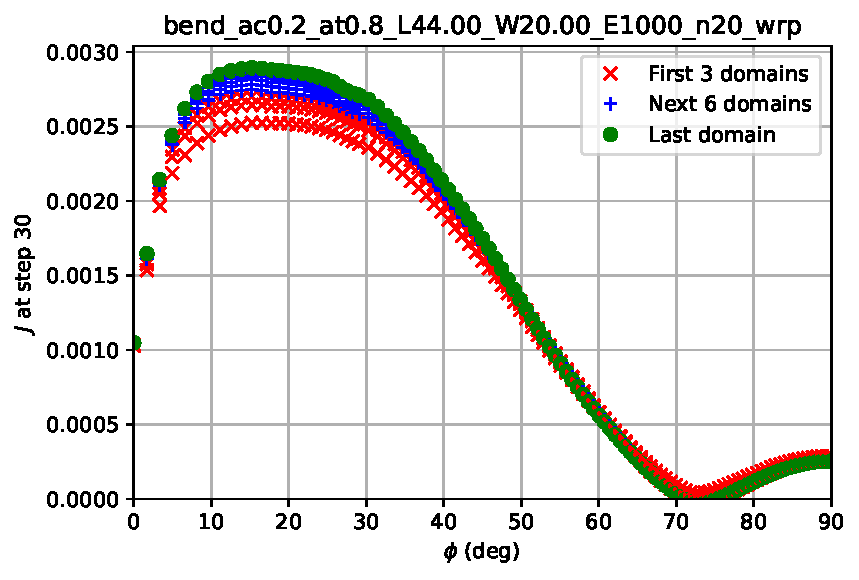
\includegraphics[width=\columnwidth]{negative_J}
\caption{Anomalous \J convergence graph}
\end{figure}
\end{column}
\end{columns}
\note{
During the \J convergence study, some of the models had local minima in the \J values at weird locations, like the one on the right.
\vfill
They did converge well as we used more elements around the crack front, but converged to unexpected values sometimes.
\vfill
}
\end{frame}

\subsection{Addition of Elastic Boundary at Crack Face}

\begin{frame}
Why is \J higher at \(\phi=90\) in some cases? What happens to plate deflection?
\begin{columns}
\begin{column}{0.45\textwidth}
\begin{figure}[tbp]
\centering
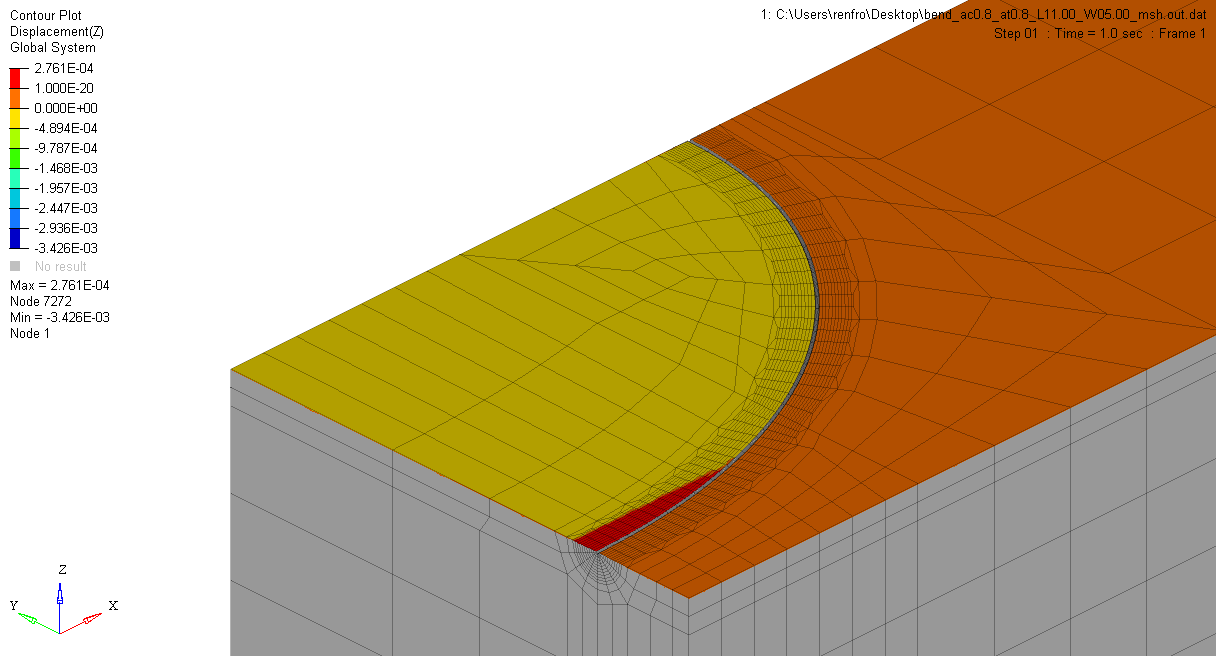
\includegraphics[width=\columnwidth]{step-01-zoomed}
\caption{First load step}
\end{figure}
\end{column}
\begin{column}{0.45\textwidth}
\begin{figure}[tbp]
\centering
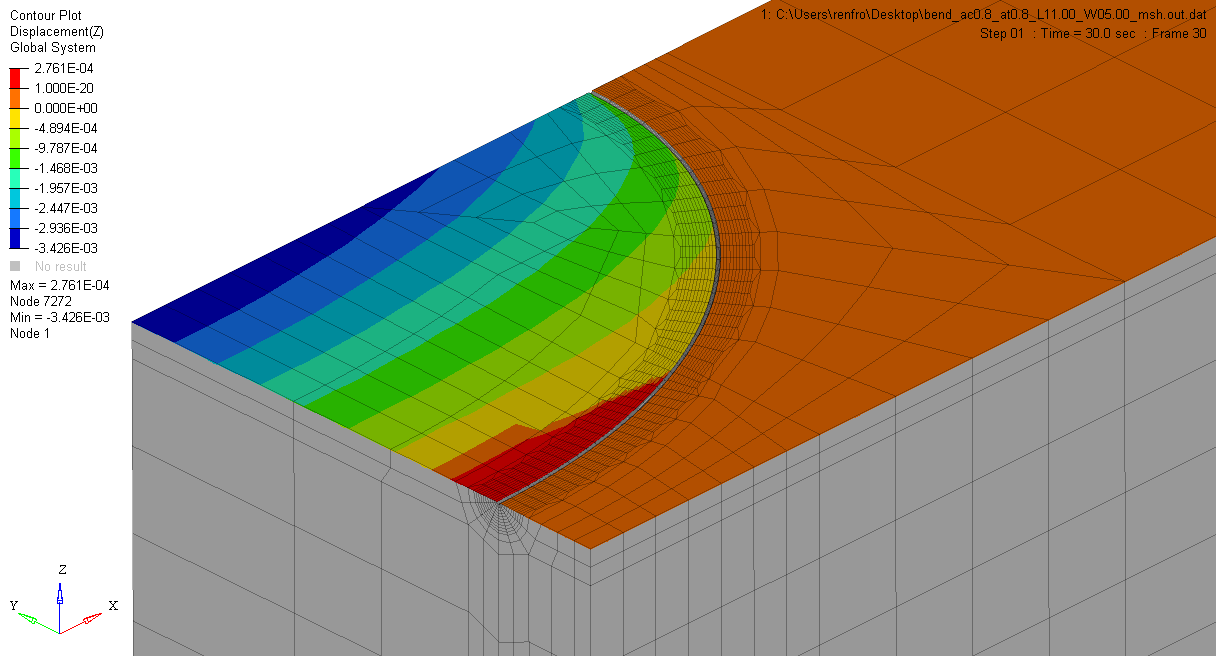
\includegraphics[width=\columnwidth]{step-30-zoomed}
\caption{Last load step}
\end{figure}
\end{column}
\end{columns}
\note{
Looking at how the plate deformed,
\vfill
where orange is basically zero deflection,
\vfill
red is positive deflection, and
\vfill
yellow and below are negative deflections,
\vfill
it's clear that regions deep in the crack are pushing out past the symmetry plane, which is physically impossible.
\vfill
This never happens on tension models, as the plate cross section is always being stretched. But in bending, the underside of the plate is effectively being compressed, and it's pushing some of the cracked material along with it.
\vfill
}
\end{frame}

\begin{frame}
\begin{figure}[tbp]
\centering
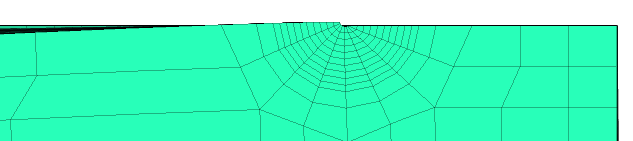
\includegraphics[width=0.9\columnwidth]{left-step-30-10x-zoomed-before.png}
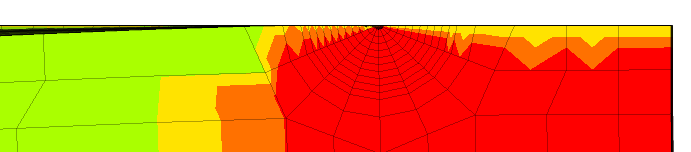
\includegraphics[width=0.9\columnwidth]{left-step-30-10x-zoomed-after.png}
\caption{Plate deflection before and after addition of elastic boundary}
\end{figure}
\note{
So an elastic boundary was added to the symmetry plane.
\vfill
A rigid boundary plane would be more common, but WARP3D doesn't support those.
\vfill
The effect of the boundary on displacement can be seen here, where now all the plate material stays below the symmetry plane.
\vfill
}
\end{frame}

\begin{frame}
\begin{columns}
\begin{column}{0.45\columnwidth}
\begin{figure}[tbp]
\centering
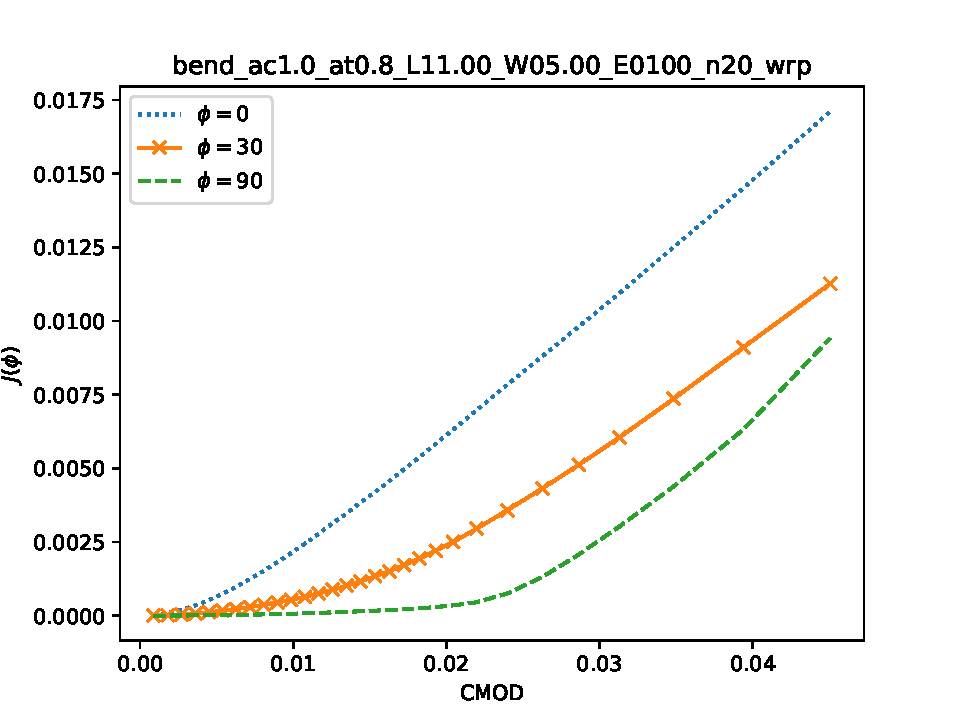
\includegraphics[width=\columnwidth]{before-J_CMOD_bend_ac10_at08_L1100_W0500_E0100_n20_wrp}
\caption{Before addition of elastic boundary}
\end{figure}
\end{column}
\begin{column}{0.45\columnwidth}
\begin{figure}
\centering
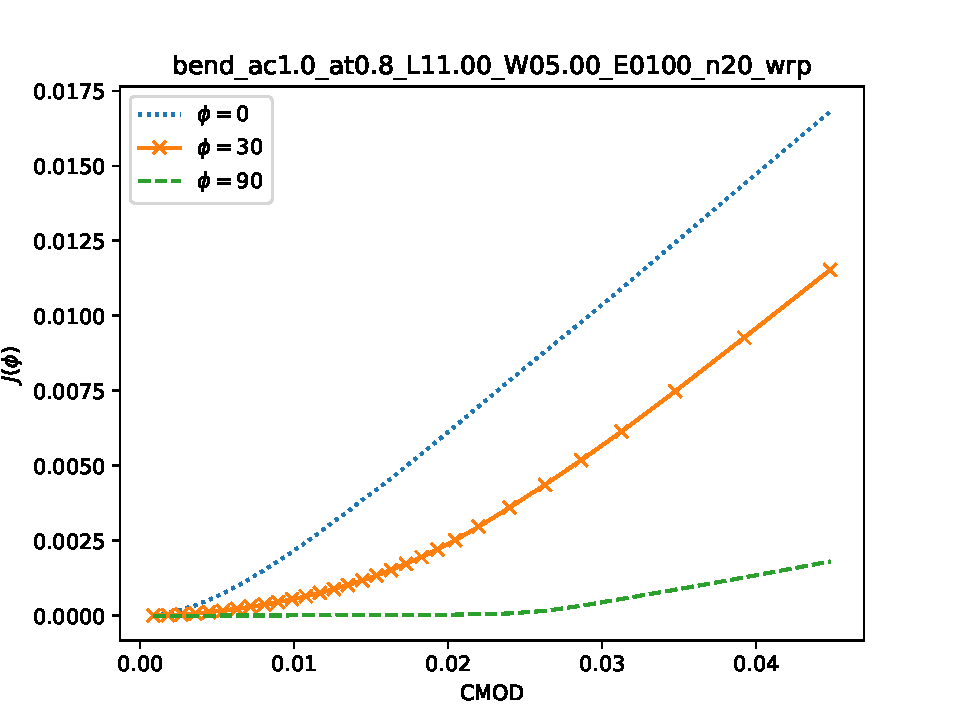
\includegraphics[width=\columnwidth]{after-J_CMOD_bend_ac10_at08_L1100_W0500_E0100_n20_wrp}
\caption{After addition of elastic boundary}
\end{figure}
\end{column}
\end{columns}
\note{
In terms of \J values, the plane has no effect toward the free surface (the solid and dotted lines),
\vfill
but greatly reduces the \J values seen deep in the crack (the dashed line)
\vfill
}
\end{frame}

\begin{frame}
\begin{columns}
\begin{column}{0.45\columnwidth}
\begin{figure}[tbp]
\centering
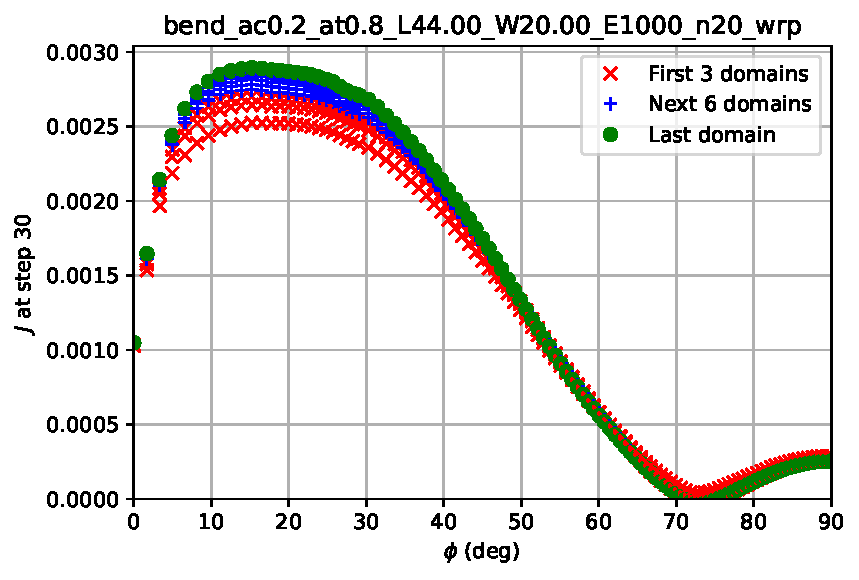
\includegraphics[width=\columnwidth]{negative_J}
\caption{Before addition of elastic boundary}
\end{figure}
\end{column}
\begin{column}{0.45\columnwidth}
\begin{figure}
\centering
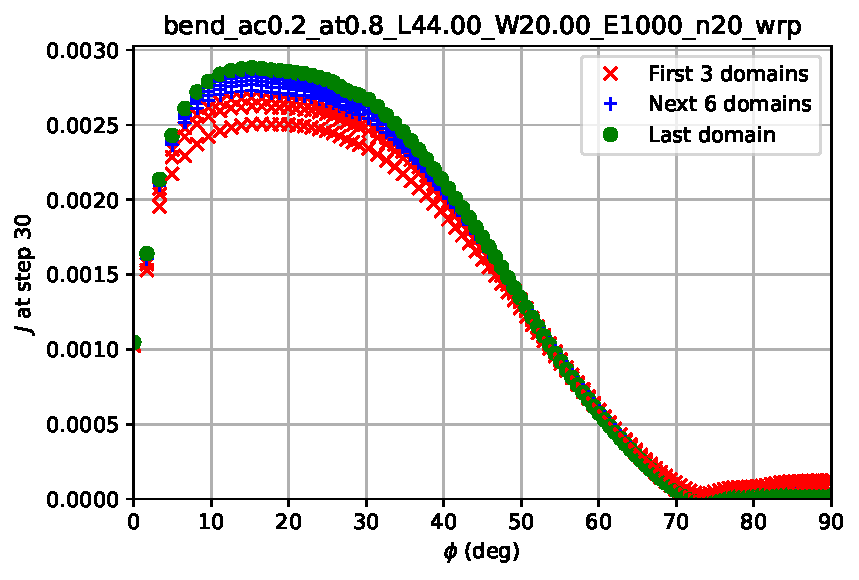
\includegraphics[width=\columnwidth]{negative_J_corrected}
\caption{After addition of elastic boundary}
\end{figure}
\end{column}
\end{columns}
\note{
Looking at the effect on \J around the crack front, it's clear this removed the local minimum for \J that was the original symptom of the problem.
\vfill
}
\end{frame}

\section{Validation of Purpose-Built Model Results}

\begin{frame}
\begin{columns}
\begin{column}{0.45\textwidth}
\begin{figure}[tbp]
\centering
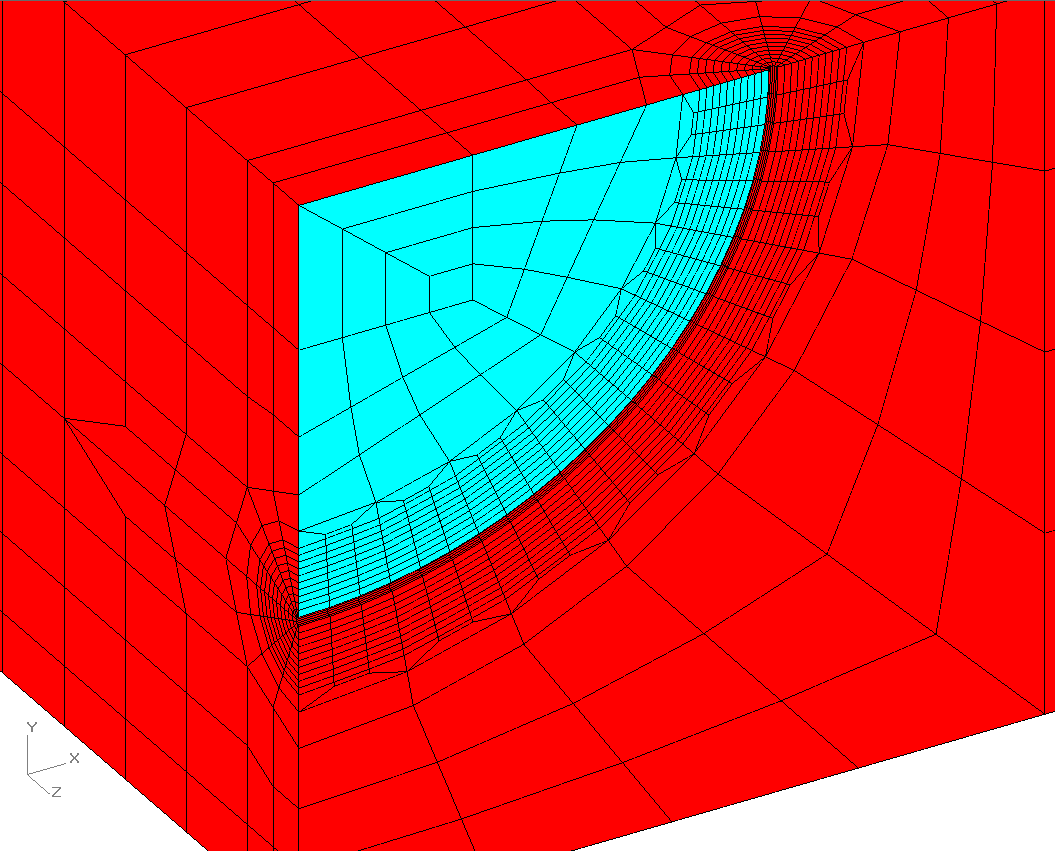
\includegraphics[width=\columnwidth]{exp_validation_mesh_zoomed}
\caption{Crack front mesh of purpose-built experimental validation model}
\end{figure}
\end{column}
\begin{column}{0.45\textwidth}
\begin{figure}[tbp]
\centering
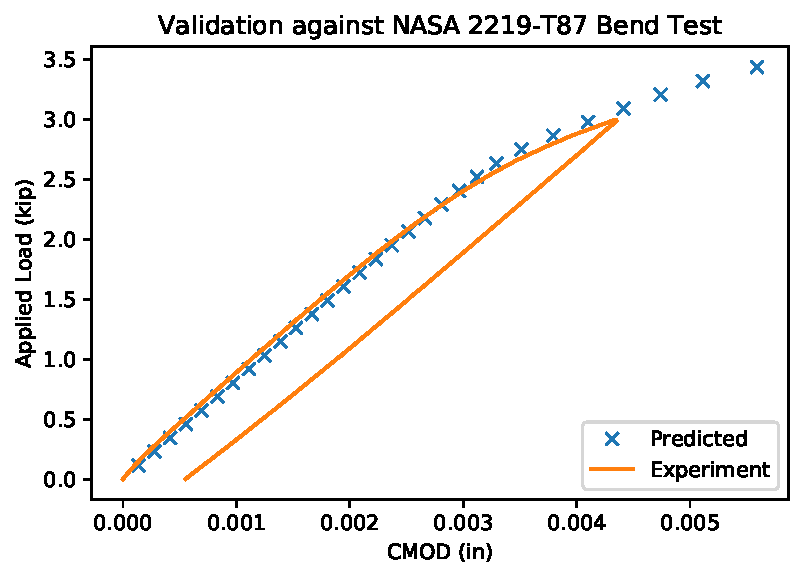
\includegraphics[width=\columnwidth]{experimental-validation-load-cmod}
\caption{Comparison of predicted load and CMOD between purpose-built model and experiment}
\end{figure}
\end{column}
\end{columns}
\note{
Next up is making sure that FEACrack and WARP3D can reproduce a load-displacement curve from a four-point bend experiment.
\vfill
A plate model with the right material properties and a crack of the correct depth and aspect ratio was created, and the blue x marks show its load-CMOD curve.
\vfill
The solid line represents a NASA four-point bend experiment, and matches the prediction within a few percent at most.
\vfill
}
\end{frame}

\section{Validation of Modified TASC Output}

\begin{frame}
\begin{columns}
\begin{column}{0.45\textwidth}
\begin{figure}[tbp]
\centering
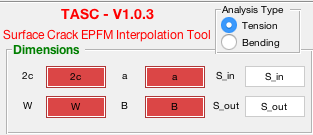
\includegraphics[width=0.8\columnwidth]{tasc-modified-ui} \vspace{1ex}
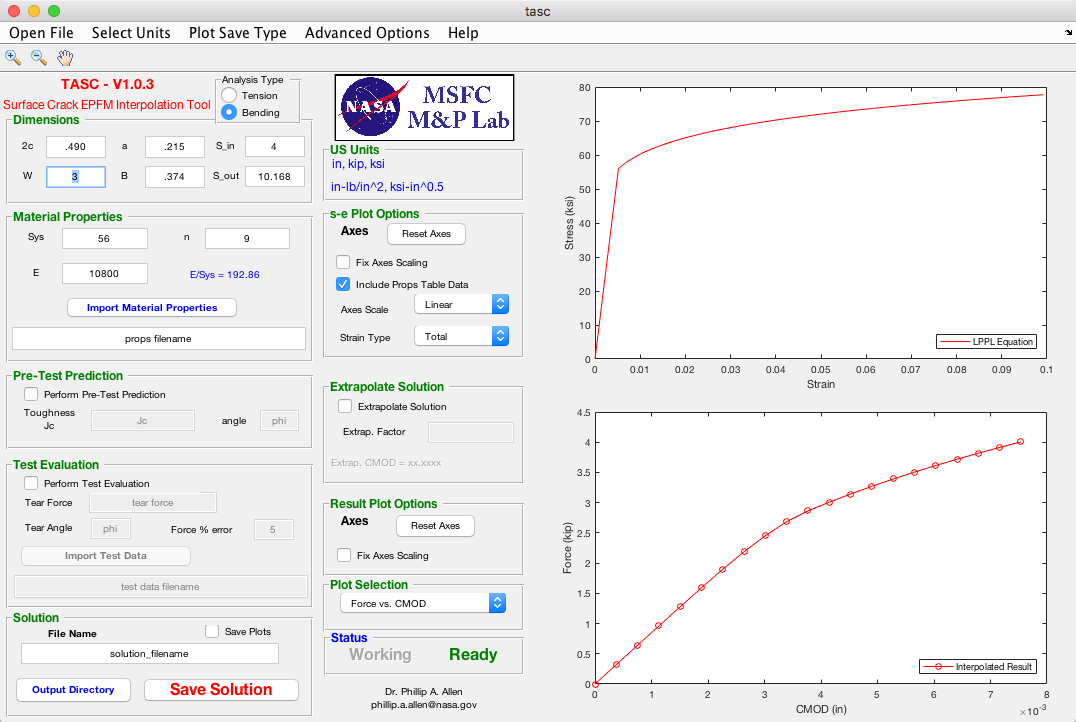
\includegraphics[width=0.8\columnwidth]{tasc-force-cmod-validation}
\caption{Modified TASC Program}
\end{figure}
\end{column}
\begin{column}{0.45\textwidth}
\begin{figure}[tbp]
\centering
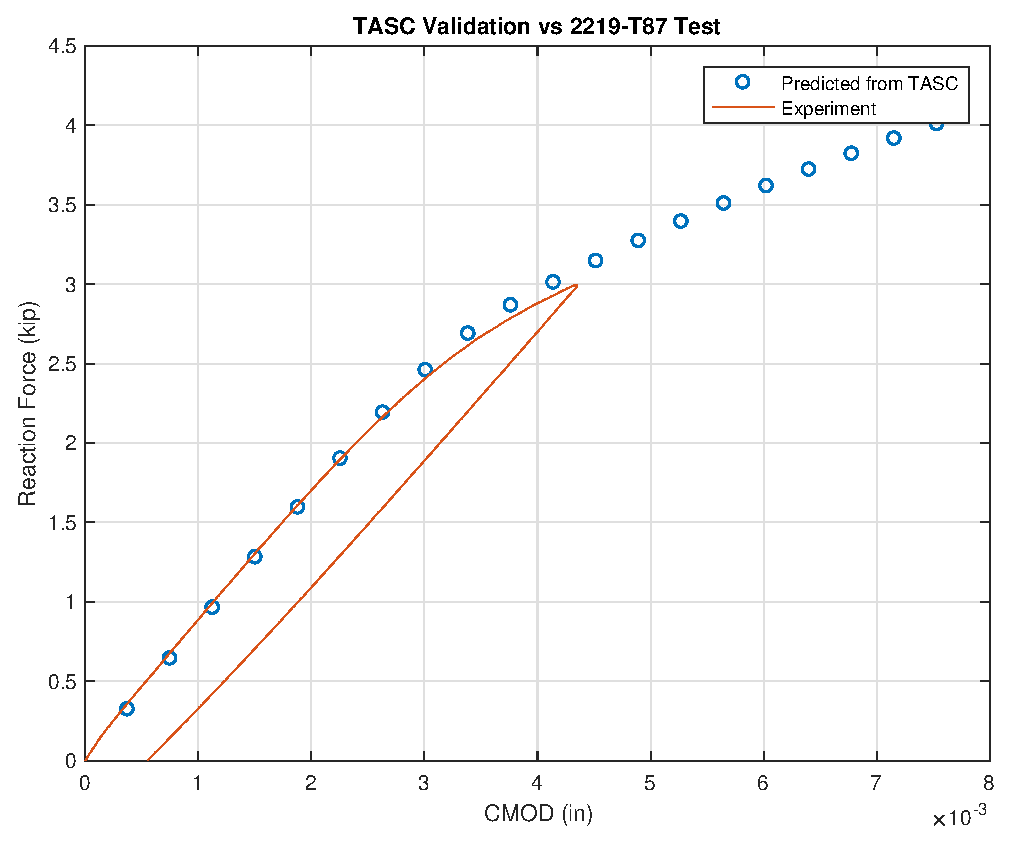
\includegraphics[width=0.75\columnwidth]{experimental-validation}
\caption{Comparison of TASC and experiment}
\end{figure}
\end{column}
\end{columns}
\note{
Finally, in terms of TASC work, the very minimal user interface changes can be seen in the top left,
\vfill
where a radio button switching between tension and bending analysis has been added,
\vfill
as well as two text entries for roller spans.
\vfill
After entering in the correct crack geometry, plate dimensions, and material properties, the bottom left figure shows the predicted load-CMOD curve.
\vfill
The same curve is shown on the right and compared to the original experimental data.
\vfill
Again, the prediction is within percentage points all along the experimental curve.
\vfill
}
\end{frame}

\section{Validation of \J Values between WARP3D and Abaqus}

\begin{frame}
\begin{columns}
\begin{column}{0.45\columnwidth}
\begin{figure}[tbp]
\centering
\includegraphics[width=\columnwidth]{{abq_bc_ac02_at02}}
\caption{Sample Abaqus validation model}
\end{figure}
\end{column}
\begin{column}{0.45\columnwidth}
\begin{figure}[tbp]
\centering
\includegraphics[width=\columnwidth]{{abq_wrp_ac02_at08_E1000_n20}}
\caption{Sample \J comparison between Abaqus and WARP3D}
\end{figure}
\end{column}
\end{columns}
\note{
For validating \J values from WARP3D against Abaqus, you can see a representative model on the left figure.
\vfill
A rigid plane has been added similar to the elastic boundary added in WARP3D.
\vfill
Looking at some of the \J values from Abaqus shown with solid markers, versus the WARP3D results shown with lines,
\vfill
the \J values are coincident except at the free surface where \(\phi=0\), and even those are pretty close.
\vfill
}
\end{frame}

\section{EPRI \hone}

\begin{frame}
Previous tension cases used all elements in crack plane for fully-plastic check. Bending cases must use a smaller set since so many elements will be near the neutral axis.
\begin{columns}
\begin{column}{0.45\textwidth}
\begin{figure}[tbp]
\centering
\includegraphics[width=\columnwidth]{{check_fp_elements}}
\caption{Element set used for fully-plastic check}
\end{figure}
\end{column}
\begin{column}{0.45\textwidth}
\begin{figure}[tbp]
\centering
\includegraphics[width=\columnwidth]{{all_elements}}
\caption{All elements shown for context}
\end{figure}
\end{column}
\end{columns}
\note{
For the EPRI \hone work using Abaqus' automatic check for fully-plastic behavior,
\vfill
we restrict the fully-plastic check to just a group of elements around the crack front.
\vfill
Tension models often would use the uncracked portion of the symmetry plane, but in bending, too many of these elements would have very low bending stress applied.
\vfill
}
\end{frame}

\begin{frame}
Abaqus \J values are roughly double WARP3D values due to higher boundary condition values
\begin{columns}
\begin{column}{0.45\columnwidth}
\begin{figure}[tbp]
\centering
\includegraphics[width=\columnwidth]{{bend_ac02_at02_E0100_n03_wrp_J_converge_abs}}
\caption{WARP3D}
\end{figure}
\end{column}
\begin{column}{0.45\columnwidth}
\begin{figure}[tbp]
\centering
\includegraphics[width=\columnwidth]{bend_ac02_at02_E0100_n03_phi_J_abq}
\caption{Abaqus with fully-plastic checks}
\end{figure}
\end{column}
\end{columns}
\note{
The \J values from Abaqus have the same trend as the ones from WARP3D, but they're about twice as large due to extra load being applied to satisfy the fully-plastic check.
\vfill
}
\end{frame}

\begin{frame}
Abaqus \hone values scale with \J as expected
\begin{figure}[tbp]
\centering
\includegraphics[width=0.6\columnwidth]{bend_ac02_at02_E0100_n03_phi_h1}
\end{figure}
\note{
The \hone values scale with \J as expected.
\vfill
}
\end{frame}

\begin{frame}
\hone results from WARP3D are \(E\)-dependent to various degrees
\begin{columns}
\begin{column}{0.45\columnwidth}
\begin{figure}[tbp]
\centering
\includegraphics[width=0.9\columnwidth]{h1_warp_ac02_at02_n03}
\caption{\(\frac{a}{c}=0.2, \frac{a}{t}=0.2, n=3\)}
\end{figure}
\end{column}
\begin{column}{0.45\columnwidth}
\begin{figure}[tbp]
\centering
\includegraphics[width=0.9\columnwidth]{h1_warp_ac02_at02_n20}
\caption{\(\frac{a}{c}=0.2, \frac{a}{t}=0.2, n=20\)}
\end{figure}
\end{column}
\end{columns}
\note{
In theory, \hone values should not be dependent on \(E\), but the WARP3D \hone values vary across \(E\) values to some degree.
}
\end{frame}

\begin{frame}
Abaqus \hone values with fully-plastic check are \(E\)-dependent
\begin{columns}
\begin{column}{0.45\textwidth}
Needed higher stress to achieve fully-plastic state
\begin{itemize}
\item \(E=100, \sigma=1.64\)
\item \(E=200, \sigma=2.27\)
\item \(E=500, \sigma=3.36\)
\item \(E=1000, \sigma=4.41\)
\end{itemize}

\end{column}
\begin{column}{0.45\textwidth}
\begin{figure}[tbp]
\centering
\includegraphics[width=\columnwidth]{bend_ac02_at02_n03_phi_h1}
\end{figure}
\end{column}
\end{columns}
\note{
In Abaqus, the applied stress values increase with \(E\), and that helps drive its \hone values progressively lower.
\vfill
}
\end{frame}

\section{Load Separation}

\subsection{Load Separation in Bending}

\begin{frame}
\begin{columns}
\begin{column}{0.45\textwidth}
\begin{figure}[tbp]
\centering
\includegraphics[width=\columnwidth]{Sij_spread_at_06}
\caption{Variation of \Sij for cracked plates in bending, \(\frac{a}{t}=0.6\) \label{fig:Sij_spread_at_06}}
\end{figure}
\end{column}
\begin{column}{0.45\textwidth}
\begin{figure}[tbp]
\centering
\includegraphics[width=\columnwidth]{Sij_bet_full_E0500_n04}
\caption{Variation of \Sij versus effective uncracked ligament length (bending, \(0.2 \leq \frac{a}{t} \leq 0.8\)) \label{fig:Sij_bet_full_E0500_n04}}
\end{figure}
\end{column}
\end{columns}
\note{
On the left is one set of separation parameters for cracks with \(\frac{a}{t}=0.6\).
\vfill
They're nearly constant across the range of CMOD values.
\vfill
On the right is all 20 separation parameters plotted against the effective uncracked ligament length used previously.
\vfill
They obviously don't lie on a single line. At best, they're self-similar at a given depth, but not across depths.
\vfill
}
\end{frame}

\subsection{Further Investigation into Load Separation in Tension}

\begin{frame}
\begin{columns}
\begin{column}{0.45\textwidth}
\begin{figure}[tbp]
\centering
\includegraphics[width=\columnwidth]{cmodpl_Sij_tension_14}
\caption{Separation parameters for cracked plates in tension}
\end{figure}
\end{column}
\begin{column}{0.45\textwidth}
\begin{figure}[tbp]
\centering
\includegraphics[width=\columnwidth]{bet_Sij_tension_14_annotated}
\caption{Variation in \Sij versus effective uncracked ligament length (tension, \(0.2 \leq \frac{a}{t} \leq 0.8\))}
\end{figure}
\end{column}
\end{columns}
\note{
Looking at 14 tension models including at least two examples of each depths and aspect ratio, they show the same trend:
\vfill
Each group of points at a given depth follow a trend, but trends do not extend across depths.
\vfill
Looking at the points closest to the original \citet{sharobeamlandes1994} results, it may be that their data sets were too sparse to see the more complete trend.
\vfill
}
\end{frame}

\part{Conclusions and Recommendations for Future Work%
\note{Time check: be at 30--35 minute mark here.
\vfill
So what conclusions can we draw, and where do we go from here?
\vfill}%
}

\section{Conclusions}

\begin{frame}
\begin{columns}
\begin{column}{0.6\textwidth}
\begin{enumerate}
\item Database of 600 elastic-plastic finite element results for surface cracks in bending
\begin{itemize}
\item More challenging than tension models
\item Subset of results verified and validated against Abaqus and experimental data
\item Modified TASC program
\item Possible to satisfy requirements of ASTM E2899 for tension {\bfseries and} bending without constructing purpose-built EPFM models
\item Greatly reduces analytical burden on anyone doing ASTM E2899 tests
\end{itemize}
\end{enumerate}
\end{column}
\begin{column}{0.3\textwidth}
\begin{figure}[tbp]
\centering
\includegraphics[width=0.8\columnwidth]{tasc-force-cmod-validation}
\end{figure}
\begin{figure}[tbp]
\centering
\includegraphics[width=0.75\columnwidth]{experimental-validation}
\end{figure}
\end{column}
\end{columns}
\note{
First and foremost, we now have a database of 600 elastic-plastic FEA results for surface cracks in bending.
\vfill
These models had some extra challenges compared to tension models, and those were overcome.
\vfill
A subset of the results have been verified and validated against Abaqus models and against experimental data
\vfill
The TASC program has been modified to support bending, at least as far as predicting load-CMOD curves.
\vfill
All of this means it's now possible to satisfy all the requirements of ASTM E2899 in both tension and bending, without building custom models for each test,
\vfill
and this greatly reduces the analytical burden on anyone performing tests under ASTM E2899.
\vfill
}
\end{frame}

\begin{frame}
\begin{columns}
\begin{column}{0.45\textwidth}
\begin{enumerate}\setcounter{enumi}{1}
\item \hone curve may not always be independent of \(E\)

\begin{itemize}
\item But \(\hone = \frac{\Jpl}{\alpha \sigma_0 \epsilon_0 t \left( \frac{\sigma}{\sigma_0}\right)^{n+1}} \) has no \(E\), and neither do any of the handbook curves
\item Abaqus fully-plastic checks are not a cure-all for finding \hone
\end{itemize}
\end{enumerate}
\end{column}
\begin{column}{0.45\textwidth}
\begin{figure}[tbp]
\centering
\includegraphics[width=\columnwidth]{h1_warp_ac10_at08_n03}
\end{figure}
\end{column}
\end{columns}
\note{
In the area of EPRI \hone, it looks like there's some dependence on \(E\) which was unexpected.
\vfill
The check for fully-plastic conditions in Abaqus is not magic. 
\vfill
}
\end{frame}

\begin{frame}
\begin{columns}
\begin{column}{0.45\textwidth}
\begin{enumerate}\setcounter{enumi}{2}
\item Load separation does not collapse to a single key curve
\begin{itemize}
\item Load separation data is self-similar at a single depth, but not across multiple depths
\item Applies to surface cracks in both tension and bending
\end{itemize}
\end{enumerate}
\end{column}
\begin{column}{0.45\textwidth}
\begin{figure}[tbp]
\centering
\includegraphics[width=\columnwidth]{bet_Sij_tension_14_annotated}
\end{figure}
\end{column}
\end{columns}
\note{
And in the area of load separation, examining a broader set of models indicated that a single-specimen technique is more complicated than first thought,
\vfill
as separation parameters don't lie on a single curve fit.
\vfill
}
\end{frame}

\section{Recommendations for Future Work}

\begin{frame}
\begin{enumerate}
\item TASC and E2899
\begin{itemize}
\item Finish integrating bend data into TASC, beyond load-CMOD validation
\item Additional values for material and/or crack geometry
\item Investigate other interpolation methods (piecewise cubic?)
\item Replace traction boundary conditions with rigid rollers and contact modeling
\end{itemize}
\item EPRI \hone
\begin{itemize}
\item Further investigation into limits of \hone estimates
\item Geometry, boundary conditions (types and magnitudes), materials
\end{itemize}
\item Load separation
\begin{itemize}
\item Alternative to R6 $\frac{b_\text{e}}{t}$ that drives \Sij to a single curve
\end{itemize}
\item {\bfseries More experimental data needed for all of these.}
\end{enumerate}
\note{
For future work related to this research,
\vfill
there's still some work to be done in TASC modifications and testing, as I didn't modify anything beyond what was necessary to validate a load-CMOD curve
\vfill
some additional data points for crack geometry and material models may be worthwhile,
\vfill
as well as seeing if an alternative interpolation method will provide better agreement with experimental results.
\vfill
As WARP3D supports contact modeling, it may be worth replacing the traction conditions used in bending models with contact modeling of rigid rollers to more closely match experimental conditions
\vfill
For EPRI \hone estimation, we need some more detailed examination of its limitations, or where I may have a mistake in my current models
\vfill
Limitations could be related to crack shape, tension versus bending, or material properties.
\vfill
Finally, for load separation, there may be an alternative length measure other than the one from R6 that will collapse the \Sij values onto a single curve.
\vfill
Now for either of the EPRI \hone or the load separation items, each of those could be someone's dissertation on their own, especially if experiments are involved.
\vfill
And more experimental data is needed for all of these items. It's pretty sparse, and will improve confidence with any numerical method.
\vfill
}
\end{frame}

\begin{frame}[plain]
\vfill
Thanks to:
\begin{itemize}
\item Committee: Dr. Chris Wilson, Dr. Brian O'Connor, Dr. Sally Pardue, Dr. Guillermo Ramirez, Dr. Dale Wilson
\item Center for Manufacturing Research (Mechanical Properties Testing, Materials Characterization, Computer Aided Engineering)
\item Information Technology Services (High Performance Computing)
\item Dr. Phillip Allen and ASTM Committee E08 on Fatigue and Fracture
\item Friends and family
\end{itemize}
\vfill
\note{
That's it for the presentation.
\vfill
I'd like to thank Dr. Chris Wilson and my committee members: Dr. Brian O'Connor, Dr. Sally Pardue, Dr. Guillermo Ramirez, and Dr. Dale Wilson.
\vfill
Facilities from both the Center for Manufacturing Research and Information Technology Services were instrumental at different phases of this research.
\vfill
Dr. Phillip Allen and ASTM Committee E08 provided a foundation for my research, and hopefully a permanent home for its results.
\vfill
And finally, my friends and family who have been consistently encouraging through this whole thing.
\vfill
Any questions?
\vfill
}
\end{frame}

\appendix

\begin{frame}[plain]
% Last-minute adjustments:
% - get titles and frame numbers for start of each chapter,
% - adjust the NavigationX numbers and titles below to match,
% - rebuild the presentation PDF.
\begin{itemize}
\item \structure{\hyperlink{Navigation39}{Introduction to Fracture Mechanics}}
\item \structure{\hyperlink{Navigation42}{Initial Verification of Quillen Models}}
\item \structure{\hyperlink{Navigation44}{Initial Verification of Two Tension Cases from \citet{allenwells2014}}}
\end{itemize}
\end{frame}

\part{Introduction to Fracture Mechanics}

\section{Basics of Fracture Mechanics}

\begin{frame}
\begin{columns}
\begin{column}{0.45\textwidth}
  \begin{align*}
    \G &= - \frac{d \Pi}{dA} = \frac{\pi \St^2 a}{E'} = \frac{\KI^2}{E'} \\
    \intertext{where}
    A &= 2at = \textnormal{area of cracked surfaces} \\
    E' &= 
    \begin{cases}
      E & \textnormal{for plane stress} \\
      \frac{E}{(1-\nu^2)} & \textnormal{for plane strain}
    \end{cases} \\
    \KI &= \St \sqrt{\pi a}.
  \end{align*}
  \begin{align*}
\Sxx(r,0) &= \Syy(r,0) = \Sone(r,0) = \Stwo(r,0) = \frac{\KI}{\sqrt{2\pi r}}
\end{align*}
\(\Sxx = \Syy = \Sone = \Stwo = \infty\) at \(r=0\).

\end{column}
\begin{column}{0.45\textwidth}
\begin{figure}
\centering
\includegraphics[width=0.6\columnwidth]{through-crack-infinite-plate}
\caption{A through crack in an infinite plate loaded in tension}
\end{figure}
\end{column}
\end{columns}
\end{frame}

\begin{frame}
  \begin{align*}
  \ry &=
    \begin{cases}
      \frac{1}{2\pi} \left( \frac{\KI}{\Sys} \right)^2 & \textnormal{for plane stress} \\
      \frac{1}{6\pi} \left( \frac{\KI}{\Sys} \right)^2 & \textnormal{for plane strain.} \\
    \end{cases}
  \end{align*}
  \begin{align*}
  \rp &=
    \begin{cases}
      \frac{1}{\pi} \left( \frac{\KI}{\Sys} \right)^2 & \textnormal{for plane stress} \\
      \frac{1}{3\pi} \left( \frac{\KI}{\Sys} \right)^2 & \textnormal{for plane strain.}
    \end{cases}
  \end{align*}
\begin{align*}
\aapp &= a+\ry = a + \frac{\rp}{2}
\end{align*}
\begin{align*}
K_{\textnormal{Iapp}} &= \St \sqrt{\pi \aapp}
\end{align*}
\end{frame}

\section{The Surface Crack Problem}

\begin{frame}
\begin{columns}
\begin{column}{0.45\textwidth}
at \(\phi=\frac{\pi}{2}\)
\begin{align*}
\KI   &= 1.1 \St \sqrt{\pi a} \left[ F \left(\frac{a}{c},\frac{\St}{\Sys}\right) \right]\\
      \intertext{where}
F\left(\frac{a}{c},\frac{\St}{\Sys}\right) &= \left[\Phi^2 - 0.212 \left(\frac{\St}{\Sys}\right)^2\right]^{-0.5} \\
\Phi &= \Int{\sqrt{\left[ \sin^2 \phi + \left(\frac{a}{c}\right)^2 \cos^2 \phi \right]}}{\phi,0,\frac{\pi}{2}}
\end{align*}
\(\frac{c}{W} \ll 1\), \(\frac{a}{c} < 1\), \(\frac{a}{t} < 0.5\)
\end{column}
\begin{column}{0.45\textwidth}
\begin{align*}
\Phi^2 &= Q = 1 + 1.464 \left( \frac{a}{c} \right)^{1.65}
\end{align*}
\end{column}
\end{columns}
\end{frame}

\subsection{Early Efforts to Quantify Effects of Finite Thickness}

\begin{frame}
\begin{figure}
\centering
\includegraphics[width=0.5\columnwidth]{wang-parks-line-spring}
\caption{\label{fig:wang-parks-line-spring} Line spring model \citep{wangparks1992}. (a) Through-cracked plate with line-spring of width \(2c\), (b) Part-through-cracked plane strain plate of comparable compliance to line-spring plate}
\end{figure}
\end{frame}

\subsection{The Newman-Raju Equation for Stress Intensity Factors}

\begin{frame}
\begin{align*}
K &= \KI = \St \sqrt{\left( \pi \frac{a}{Q}\right) F\left(\frac{a}{t},\frac{a}{c},\phi\right)}
\end{align*}
\begin{columns}
\begin{column}{0.45\textwidth}
\begin{figure}
\centering
	   \includegraphics[width=0.6\columnwidth]{newman-raju-figure-5}
      \caption{$Q=\frac{\pi^2}{4}$, $\frac{a}{t}=0.8$}
\end{figure}
\end{column}
\begin{column}{0.45\textwidth}
\begin{figure}
\centering
	   \includegraphics[width=0.6\columnwidth]{newman-raju-figure-6}
      \caption{$Q=1.104$, $\frac{a}{t}=0.8$, $\frac{a}{c}=0.2$}
\end{figure}
\end{column}
\end{columns}
\end{frame}

\begin{frame}
\begin{columns}
\begin{column}{0.45\textwidth}
\begin{figure}
\centering
	   \includegraphics[width=\columnwidth]{3_meshes}
      \caption{Comparison of wedge sizes used in estimating bound\-ary-layer effect}
      \label{fig:wedge_refinement}
\end{figure}
\end{column}
\begin{column}{0.45\textwidth}
\begin{figure}
\centering
	   \includegraphics[width=0.8\columnwidth]{nr_fig7}
      \caption{Effects of mesh refinement near the free surface on the distribution of bound\-ary-cor\-rec\-tion factors for semi-circu\-lar surface crack ($Q=\frac{\pi^2}{4}$; $\frac{a}{t}=0.2$)}
\end{figure}
\end{column}
\end{columns}
\end{frame}

\begin{frame}
\begin{columns}
\begin{column}{0.45\textwidth}
\begin{figure}
\centering
	   \includegraphics[width=0.8\columnwidth]{nr_fig8}
      \caption{$Q=\frac{\pi^2}{4}$}
\end{figure}
\end{column}
\begin{column}{0.45\textwidth}
\begin{figure}
\centering
	   \includegraphics[width=0.8\columnwidth]{nr_fig9}
      \caption{$Q=1.104$, $\frac{a}{c}=0.2$}
\end{figure}
\end{column}
\end{columns}
\begin{align*}
\KI &= \St \sqrt{F\left(\frac{a}{t},\frac{a}{c},\phi\right) \left( \pi \frac{a}{Q}\right)}
\end{align*}
\end{frame}

\subsection{Elastic-Plastic Fracture}

\begin{frame}
\begin{figure}
\centering
\includegraphics[width=0.5\columnwidth]{ctod-irwin}
\caption{Estimation of CTOD from displacement field of crack with Irwin plastic radius correction}
\end{figure}
\begin{align*}
\deltat &= 2 u_{y} = \frac{8}{E'} \KI \sqrt{\frac{\ry}{2\pi}}
\end{align*}
\end{frame}

\begin{frame}
\begin{columns}
\begin{column}{0.45\textwidth}
\begin{figure}
\centering
\includegraphics[width=\columnwidth]{contour-integral}
\end{figure}
\end{column}
\begin{column}{0.45\textwidth}
\begin{align*}
\J &= \int_{\Gamma} \left( w \, {dy} - T_i \pderiv{u_i}{x} \, {ds}\right)
\end{align*}
where
\begin{align*}
w &= \textnormal{strain energy density} \\
T_i &= \textnormal{components of traction vector} \\
u_i &= \textnormal{components of displacement vector} \\
ds &= \textnormal{differential length along \(\Gamma\)}
\end{align*}
\end{column}
\end{columns}
\end{frame}

\begin{frame}
\begin{columns}
\begin{column}{0.45\textwidth}
\begin{align*}
J &= - \D{\Pi}{A}
\intertext{where}
dA &=
  \begin{cases}
  t \,da & \textnormal{edge-cracked plate} \\
  2 t \,da & \textnormal{center-cracked plate} \\
  2\pi a \,da & \textnormal{embedded circular crack}
  \end{cases}
\intertext{and}
\Pi &= U - F
\end{align*}
\end{column}
\begin{column}{0.45\textwidth}
where \(U\) is the strain energy stored in the body and \(F\) is the work done by the applied load \(P\).
\begin{figure}
\centering
\includegraphics[width=\columnwidth]{nonlinear-energy-release-rate}
\end{figure}
\end{column}
\end{columns}
\end{frame}

\begin{frame}
\begin{columns}
\begin{column}{0.45\textwidth}
\begin{equation*}
\frac{\epsilon}{\epsilon_0} = \frac{\sigma}{\sigma_0} + \alpha \left( \frac{\sigma}{\sigma_0} \right)^{n}
\end{equation*}
where
\begin{align*}
\sigma_0 &= \textnormal{reference stress value} \\
\epsilon_0 &= \frac{\sigma_0}{E} \\
\alpha &= \textnormal{yield offset parameter, often 0.5} \\
n &= \textnormal{strain hardening exponent}
\end{align*}
\end{column}
\begin{column}{0.45\textwidth}
\begin{figure}
\centering
\includegraphics[width=0.8\columnwidth]{ramberg-osgood}
\end{figure}
\end{column}
\end{columns}
\end{frame}


\part{Initial Verification of Quillen Models}

\begin{frame}[fragile]
\begin{columns}
\begin{column}{0.45\textwidth}
\begin{figure}[bp]
\begin{lstlisting}[language={APDL}]
! Define parameters
E=30.0e6
NU=0.3
! Set material properties
MP,EX,1,E
MP,PRXY,1,NU
\end{lstlisting}
\caption{APDL syntax \label{fig:material-apdl}}
\end{figure}
\end{column}
\begin{column}{0.45\textwidth}
\begin{figure}[bp]
\begin{lstlisting}[language={Abaqus}]
** Define parameters
*PARAMETER
E=30.0e6
NU=0.3
** Set material properties
*MATERIAL, NAME=STEEL
*ELASTIC
<E>, <NU>
\end{lstlisting}
\caption{Abaqus keyword syntax \label{fig:material-abaqus-keyword}}
\end{figure}
\end{column}
\end{columns}
\end{frame}

\begin{frame}[fragile]
\begin{figure}[bp]
\begin{lstlisting}
def setMaterial(model, E=200e9, nu=0.3): # a function
    model.Material(name='Steel')
    model.materials['Steel'].Elastic(table=((E, nu), ))
    # function ends here, main program follows

elasticModulus=30e6 # define parameters
PoissonRatio=0.3
# call functions to create model, set material
myModel = createModel(modelName='McClung-1')
setMaterial(E=elasticModulus,
            nu=PoissonRatio,
            model=myModel)
\end{lstlisting}
\caption{Abaqus Python syntax}
\end{figure}
\end{frame}

\begin{frame}
\begin{columns}
\begin{column}{0.45\textwidth}
  \begin{figure}
    \centering
    \includegraphics[width=\columnwidth]{model1-assembly}
    \caption{McClung et al. model 1\label{fig:model1-assembly}}
  \end{figure}
\end{column}
\begin{column}{0.45\textwidth}
  \begin{figure}
    \centering
    \includegraphics[width=\columnwidth]{model1-assembly-zoomed}
    \caption{McClung et al. model 1 crack front detail\label{fig:model1-assembly-zoomed}}
  \end{figure}
\end{column}
\end{columns}

\end{frame}


\part{Initial Verification of Two Tension Cases from \citet{allenwells2014}}

\section{Extracting Normalized Results from the TASC Database}

\begin{frame}
\begin{columns}
\begin{column}{0.45\textwidth}
\begin{figure}[tbp]
\centering
\includegraphics[width=0.7\columnwidth]{aspect-ratio-gap}
\caption{\label{fig:aspect-ratio-gap} Gap in results for widest aspect ratios}
\end{figure}
\end{column}
\begin{column}{0.45\textwidth}
\begin{figure}[tbp]
\centering
\includegraphics[width=0.7\columnwidth]{modulus-gap}
\caption{Gap in results for lowest \(E\) values}
\end{figure}
\end{column}
\end{columns}
\end{frame}

\begin{frame}
\begin{columns}
\begin{column}{0.45\textwidth}
\begin{figure}[bp]
\centering
\includegraphics[width=\columnwidth]{tasc-inputs}
\caption{\label{fig:tasc_fea_inputs} Raw FEA results used in TASC}
\end{figure}
\end{column}
\begin{column}{0.45\textwidth}
\begin{figure}[tbp]
\centering
\includegraphics[width=\columnwidth]{tasc-results}
\caption{\label{fig:tasc_interp_outputs} Interpolated FEA results displayed by TASC}
\end{figure}
\end{column}
\end{columns}
\end{frame}

\section{Reconstructing Model Geometry in FEACrack}

\begin{frame}
\begin{columns}
\begin{column}{0.45\textwidth}
\begin{figure}[tbp]
\centering
\includegraphics[width=\columnwidth]{mesh-iso}
\caption{\label{fig:mesh-iso} Isometric view of overall mesh}
\end{figure}
\end{column}
\begin{column}{0.45\textwidth}
\begin{figure}[tbp]
\centering
\includegraphics[width=\columnwidth]{mesh-front}
\caption{\label{fig:mesh-front} Detailed view of crack front}
\end{figure}
\end{column}
\end{columns}
\end{frame}

\section{Reconstructing Material Parameters in FEACrack}

\begin{frame}

\begin{columns}
\begin{column}{0.45\textwidth}
\begin{align*}
\frac{\epsilon}{\epsilon_\text{ys}} &= 
\begin{cases}
\begin{aligned} % https://tex.stackexchange.com/a/385172
\hspace*{0.77em} \dfrac{\sigma}{\Sys} &,\enskip \epsilon \leq \epsilon_\text{ys} \\
\left(\dfrac{\sigma}{\Sys}\right)^{n} &,\enskip \epsilon > \epsilon_\text{ys}
\end{aligned}
\end{cases}
\end{align*}
where \(\epsilon_\text{ys} = \frac{\Sys}{E}\).
\end{column}
\begin{column}{0.45\textwidth}
\begin{figure}[tbp]
\centering
\includegraphics[width=\columnwidth]{lppl}
\caption{\label{fig:lppl} Set of LPPL stress-strain curves}
\end{figure}
\end{column}
\end{columns}

\end{frame}

\section{Applying Appropriate Boundary Conditions in FEACrack}

\begin{frame}
\begin{align*}
M &= \frac{r_\phi \Sys}{\J}
\end{align*}
\begin{table}[pb]
\caption{\label{tab:displacement_values} Applied displacement values for verification models}
\centering
\begin{tabular}{S[table-format=3.0] S[table-format=1.4] S *2{S[table-format=1.4]}} \toprule
{\(\frac{E}{\Sys}\)} & {Displacement} & {\(\phi\)} & {\(M\) using \(r_{\phi a}\)} & {\(M\) using \(r_{\phi b}\)} \\ \midrule
100 & 0.1028 & \SI{30}{\degree} & 15.9833 & 36.4241 \\
    &        & \SI{90}{\degree} & 22.6234 & 15.0822 \\
200 & 0.0550 & \SI{30}{\degree} & 24.7288 & 56.3542 \\
    &        & \SI{90}{\degree} & 34.9604 & 23.3069 \\
\bottomrule
\end{tabular}
\end{table}
\end{frame}

\section{Solving Models in WARP3D}

\begin{frame}
\begin{itemize}
\item 30 load steps
\item {\ttfamily warp3d < file.inp > file.out}
\item 21.6 minutes to solve on laptop, 2.2 minutes on HPC node
\end{itemize}
\end{frame}

\section{Analyzing WARP3D Results}

\begin{frame}
Python program
\begin{itemize}
\item run {\ttfamily packet\_reader} to export displacements, forces
\item extract node 1 \(z\) displacement, double to get CMOD
\item identify nodes on \(z=0\) from input file
\item extract \(z\) reactions from all identified nodes, sum to reaction force
\item divide reaction force by plate cross section area to get stress
\end{itemize}
\end{frame}

\begin{frame}
\begin{columns}
\begin{column}{0.45\textwidth}
\begin{figure}[tbp]
\centering
\includegraphics[width=\columnwidth]{e100_verification}
\caption{\label{fig:e100_verification} Verification of stress and CMOD relationship for first model}
\end{figure}
\end{column}
\begin{column}{0.45\textwidth}
\begin{figure}[tbp]
\centering
\includegraphics[width=\columnwidth]{e100_200_verification}
\caption{\label{fig:e100_200_verification} Verification of stress and CMOD relationship for second model}
\end{figure}
\end{column}
\end{columns}
\end{frame}

\end{document}
